% =============================================================================
% Template do Relatório Final do Projeto de Aprendizagem de Máquina (pós).
% Disciplina IN1102. Oferta 2026.2 (release 2026.2.1).
% Repositório-template: projeto-final-IN1102-2026.2.
% Cada seção traz caixas \tarefagrupo{...}, visíveis no PDF, indicando o que
% escrever; substitua cada caixa pelo texto do grupo.
% Limite recomendado: 25 páginas (sem apêndices).
% Compilar com: pdflatex relatorio.tex (duas passadas).
% =============================================================================
\documentclass[11pt,a4paper]{article}
% Preâmbulo compartilhado dos artefatos LaTeX da disciplina de Aprendizagem
% de Máquina (graduação e pós-graduação).
%
% Regras editoriais: sem emojis, sem travessões, português do Brasil com
% acentuação correta. Arquivos em UTF-8 sem BOM.
%
% Conjunto de pacotes deliberadamente enxuto para garantir compilação com
% pdflatex em diferentes instalações (TeX Live, MiKTeX), sem tikz nem
% microtype.

\usepackage[utf8]{inputenc}
\usepackage[T1]{fontenc}
\usepackage[brazilian]{babel}
\usepackage{geometry}
\geometry{a4paper,margin=2.5cm}
\usepackage{graphicx}
\usepackage{booktabs}
\usepackage{xcolor}
\usepackage{enumitem}
\usepackage{caption}
\usepackage[hidelinks]{hyperref}

% Cores institucionais aproximadas (CIn-UFPE).
\definecolor{cinazul}{RGB}{0, 51, 102}
\definecolor{cinverde}{RGB}{0, 102, 51}

% Macro para título de etapa do projeto: Etapa 1 (teórica) e Etapa 2
% (experimental), com entrada correspondente no sumário.
\newcommand{\etapa}[2]{%
    \section*{Etapa #1: #2}%
    \addcontentsline{toc}{section}{Etapa #1: #2}%
}

% Macro para destacar tarefa pendente do grupo em uma caixa visível.
\newcommand{\tarefagrupo}[1]{%
    \par\medskip
    \noindent\fbox{%
        \begin{minipage}{\dimexpr\textwidth-2\fboxsep-2\fboxrule\relax}
        \textbf{Tarefa do grupo:} #1
        \end{minipage}%
    }%
    \par\medskip
}

% Macro para citar arquivos do repositório em fonte monoespaçada.
\newcommand{\arquivo}[1]{\texttt{#1}}

\hypersetup{
    pdfauthor={Prof. Leandro Maciel Almeida},
    pdfkeywords={aprendizagem de máquina, classificação tabular, projeto final}
}

\usepackage{lmodern}
\usepackage{amsmath}
\usepackage{amssymb}
\sloppy

\hypersetup{pdftitle={Relatório Final: Projeto de Aprendizagem de Máquina (IN1102, pós), 2026.2}}

\title{\bfseries Relatório Final do Projeto\\[0.3em]
       \large Disciplina de Aprendizagem de Máquina (IN1102, pós-graduação)}
\author{Grupo:\\[0.15em]
        \textbf{Douglas Araújo Silva, Felipe Araújo de Lima,}\\
        \textbf{Letícia De Albuquerque S. Leitão}\\[0.2em]
        Modelo tema: \textbf{TabICL v2}}
\date{2026.2}

\begin{document}

\maketitle
\thispagestyle{empty}

\begin{abstract}
\noindent
Este relatório apresenta a fundamentação teórica e a avaliação experimental do \textbf{TabICL v2} (\emph{Tabular In-Context Learning}), um modelo fundacional tabular baseado em Transformers pré-treinado exclusivamente sobre dados sintéticos gerados por processos causais estruturais, confrontado com três baselines clássicos de árvores de decisão impulsionadas por gradiente (LightGBM, XGBoost e CatBoost na configuração \emph{Tuned Defaults} do pacote \texttt{pytabkit}). Na Etapa~1, detalha-se a arquitetura em três estágios do TabICL v2 ($\mathrm{TF}_{\mathrm{col}}$ com \emph{Set Transformer} induzido e \emph{Target-Aware Embedding}, $\mathrm{TF}_{\mathrm{row}}$ com codificação posicional rotacional multidimensional e $\mathrm{TF}_{\mathrm{icl}}$ com atenção escalável \emph{QASSMax}), o pré-treinamento via otimizador Muon sobre o prior sintético de Cauchy/Sobolev e sua complexidade assintótica $\mathcal{O}(n^2 + n m^2)$. Na Etapa~2, executa-se um protocolo estrito de validação cruzada aninhada sobre 30 datasets de classificação da suíte TabArena-v0.1 (10 pequenos, 10 médios e 10 grandes, com 3 folds externos oficiais e 3 folds internos para busca Bayesiana via Optuna TPE de 20 trials). Na avaliação final selada ($N = 30$ datasets completos), o TabICL v2 otimizado (\texttt{group\_tuned}, controle) alcançou posto médio de $1{,}300$ na métrica primária AUC OvO (média de $0{,}8606 \pm 0{,}1166$), superando de forma estatisticamente significativa ($\alpha = 0{,}05$) o LightGBM (posto $2{,}633$, $p_{\text{Holm}} = 6{,}33 \times 10^{-5}$), o CatBoost (posto $2{,}867$, $p_{\text{Holm}} = 5{,}20 \times 10^{-6}$) e o XGBoost (posto $3{,}200$, $p_{\text{Holm}} = 3{,}59 \times 10^{-8}$) segundo o teste global de Iman-Davenport ($F_F = 20{,}695$, $p = 3{,}28 \times 10^{-10}$) e o pós-teste de Holm. Contudo, o teste pareado de Wilcoxon signed-ranks entre \texttt{group\_tuned} e a configuração padrão \texttt{group\_default} (AUC OvO média de $0{,}8607 \pm 0{,}1170$) não apontou ganho estatisticamente significativo da busca ($T = 184{,}0$, $p = 0{,}3285$), enquanto na métrica secundária pré-declarada de entropia cruzada o \texttt{group\_default} superou significativamente o \texttt{group\_tuned} em 29 dos 30 datasets ($T = 1{,}0$, $p = 3{,}73 \times 10^{-9}$) com custo computacional quase dez vezes menor ($22{,}24\text{ s}$ contra $218{,}78\text{ s}$ por fold). Conclui-se que, nos 30 datasets e sob o teto protocolar de até $10.000$ amostras de treinamento, o TabICL v2 apresentou desempenho competitivo e, em AUC OvO, superior aos baselines avaliados. A configuração padrão mostrou resultado semelhante em AUC, menor entropia cruzada e custo substancialmente inferior ao da variante otimizada; a entropia cruzada, isoladamente, não constitui prova de calibração probabilística.
\end{abstract}

\tableofcontents
\bigskip

% =============================================================================
\section{Introdução}
\label{sec:intro}

\subsection{Contexto e motivação}

Dados tabulares estruturados em linhas (instâncias) e colunas (atributos heterogêneos) constituem a modalidade predominante em aplicações industriais, financeiras, biomédicas e científicas de Aprendizagem de Máquina. Ao contrário de domínios como visão computacional e processamento de linguagem natural, nos quais arquiteturas neurais profundas baseadas em atenção consolidaram hegemonia, a aprendizagem supervisionada em dados tabulares permaneceu historicamente dominada por ensembles de árvores de decisão impulsionadas por gradiente (\emph{Gradient Boosted Decision Trees}, GBDTs), representados por sistemas como XGBoost \cite{chen2016xgboost}, LightGBM \cite{ke2017lightgbm} e CatBoost \cite{prokhorenkova2018catboost}. Estudos comparativos sistemáticos \cite{grinsztajn2022tree,mcelfresh2023when} demonstram que a superioridade histórica dos GBDTs decorre de quatro propriedades estruturais das tabelas: (i) a ausência de invariância translacional ou espacial entre colunas e a necessidade de invariância à permutação da ordem dos atributos; (ii) a presença de funções de decisão irregulares e descontínuas alinhadas aos eixos coordenados; (iii) a forte heterogeneidade de tipos (contínuos, ordinais, categóricos de alta cardinalidade), escalas numéricas, caudas pesadas e valores ausentes; e (iv) a vulnerabilidade de redes neurais densas a atributos não informativos ou ruidosos em regimes de amostra pequena e média.

Nos últimos anos, a emergência de modelos fundacionais tabulares baseados em aprendizagem em contexto (\emph{In-Context Learning}, ICL), inaugurada pelo TabPFN \cite{hollmann2023tabpfn,hollmann2025tabpfn} e expandida pelo TabICL \cite{qu2025tabicl,qu2026tabiclv2}, reformulou o paradigma de modelagem tabular. Em vez de ajustar parâmetros iterativamente por descida de gradiente em cada nova base de dados, um Transformer pré-treinado uma única vez sobre milhões de tarefas sintéticas recebe todo o conjunto de treinamento rotulado como contexto e infere diretamente a distribuição preditiva posterior aproximada das amostras de teste em uma única passagem direta (\emph{forward pass}). Avaliar rigorosamente se essa nova família de modelos fundacionais supera de fato os baselines GBDTs modernos sob um protocolo livre de vazamento de dados e com controle estatístico de comparações múltiplas motiva o presente trabalho.

\subsection{Modelo tema}

O modelo tema investigado por este grupo é o \textbf{TabICL v2} (\emph{Tabular In-Context Learning v2}), proposto por Qu, Holzmüller, Varoquaux e Le Morvan \cite{qu2025tabicl,qu2026tabiclv2} (equipe SODA, INRIA Saclay) e disponibilizado na biblioteca oficial \texttt{tabicl} (versão \texttt{2.2.0}, checkpoint pré-treinado \texttt{tabicl-classifier-v2-20260212.ckpt}). O TabICL foi concebido para superar o gargalo de complexidade bidimensional simultânea entre células do TabPFN v2, decompondo a representação tabular em três estágios sequenciais especializados: um incorporador coluna a coluna baseado em \emph{Set Transformer} com pontos indutores ($\mathrm{TF}_{\mathrm{col}}$), um agregador de interação entre atributos por linha ($\mathrm{TF}_{\mathrm{row}}$) e um preditor de aprendizagem em contexto sobre instâncias ($\mathrm{TF}_{\mathrm{icl}}$). A segunda geração (TabICL v2) introduz atenção softmax escalável sensível ao tamanho do contexto (\emph{Query-Aware Scalable Softmax}, QASSMax), agrupamento de atributos repetidos, pré-treinamento em larga escala com o otimizador matricial Muon \cite{jordan2024muon} e um prior sintético enriquecido com funções de ativação racionais de Cauchy e kernels de Sobolev.

\subsection{Contribuições do trabalho}

As contribuições deste relatório dividem-se entre as duas etapas do projeto da disciplina IN1102:
\begin{enumerate}[leftmargin=2em]
    \item \textbf{Etapa 1 (Fundamentação Teórica):} formalização matemática completa da arquitetura em três estágios do TabICL v2 ($\mathrm{TF}_{\mathrm{col}}$, $\mathrm{TF}_{\mathrm{row}}$ e $\mathrm{TF}_{\mathrm{icl}}$), do mecanismo de pré-treinamento sintético como aproximação da distribuição preditiva posterior Bayesiana, do pipeline nativo de pré-processamento e ensemble de visões ($E = 8$ estimadores por quadrado latino), da análise de complexidade assintótica de tempo e memória $\mathcal{O}(n^2 + n m^2)$ e do posicionamento frente à literatura de 2023 a 2026;
    \item \textbf{Etapa 2 (Estudo Experimental e Análise Estatística):} execução de um estudo comparativo reprodutível sobre 30 datasets estratificados da suíte TabArena-v0.1 \cite{erickson2025tabarena} contra LightGBM, XGBoost e CatBoost (\emph{Tuned Defaults} do \texttt{pytabkit} \cite{holzmuller2024better}), incluindo estudos diagnósticos de sensibilidade, ablação de componentes de ensemble, análise de sobreajuste por lacuna treino-validação e curvas de complexidade com a regra de 1 erro padrão, erros por classe e testes não paramétricos de Friedman, Iman-Davenport, Holm, Bonferroni-Dunn, Nemenyi e Wilcoxon signed-ranks \cite{demsar2006statistical} tanto na métrica primária (AUC OvO) quanto na métrica secundária pré-declarada (entropia cruzada).
\end{enumerate}

O restante do relatório está organizado como segue: a Seção~\ref{sec:etapa1} desenvolve a fundamentação teórica do TabICL v2; a Seção~\ref{sec:etapa2} descreve o protocolo experimental, os estudos de desenvolvimento e os resultados estatísticos no teste selado; a Seção~\ref{sec:discussao} discute os achados e as ameaças à validade; a Seção~\ref{sec:reprodutibilidade} documenta a reprodutibilidade e a auditoria do protocolo; e os Apêndices~\ref{app:datasets} a~\ref{app:bootstrap} apresentam as tabelas completas por base de dados e os artefatos de auditoria.

% =============================================================================
\section{Etapa 1: Fundamentação teórica do modelo}
\label{sec:etapa1}

\subsection{Motivação e contexto histórico}
\label{sec:motivacao}

O problema da classificação supervisionada tabular consiste em aprender, a partir de um conjunto de treinamento rotulado $\mathcal{D}_{\mathrm{tr}} = \{(x_i, y_i)\}_{i=1}^{n_{\mathrm{tr}}}$ com $x_i \in \mathcal{X}_1 \times \dots \times \mathcal{X}_m$ e $y_i \in \{1, \dots, C\}$, um mapeamento preditivo capaz de estimar a distribuição condicional de probabilidades $P(y_{\mathrm{te}} \mid x_{\mathrm{te}}, \mathcal{D}_{\mathrm{tr}})$ para novas instâncias de teste $x_{\mathrm{te}} \in X_{\mathrm{te}}$. Durante duas décadas, a abordagem dominante baseou-se na minimização do risco empírico regularizado sobre famílias aditivas de árvores de decisão:
\begin{equation}
    \hat{f}(x) = \sum_{t=1}^{T} \eta \, h_t(x), \qquad \text{com } h_t \in \mathcal{H}_{\text{tree}},
\end{equation}
em que cada árvore $h_t$ particiona recursivamente o espaço $\mathbb{R}^m$ por limiares ortogonais aos eixos ($x_{i,j} \le \theta$) para aproximar o gradiente negativo e a curvatura de segunda ordem da função de perda \cite{chen2016xgboost,ke2017lightgbm,prokhorenkova2018catboost}. Embora altamente eficazes e computacionalmente rápidos, os GBDTs constroem fronteiras de decisão em degraus ortogonais aos eixos, sofrem degradação quando a função alvo depende de rotações lineares ou relações suaves globais entre atributos e precisam reestimar sua estrutura do zero a cada novo dataset, o que limita sua eficiência amostral em bases pequenas.

A primeira geração de redes neurais profundas para dados tabulares tentou adaptar arquiteturas do aprendizado profundo clássico ao domínio tabular, incluindo perceptrons multicamadas regularizados e arquiteturas tipo ResNet \cite{gorishniy2021revisiting}, Transformers com tokenização por atributo como o FT-Transformer \cite{gorishniy2021revisiting}, codificações numéricas contínuas por funções periódicas ou lineares por partes \cite{gorishniy2022embeddings} e modelos híbridos com recuperação de vizinhos como o TabR \cite{gorishniy2024tabr} ou ensembles eficientes por pesos de baixo posto como o TabM \cite{gorishniy2025tabm}. Apesar dos avanços, esses modelos paramétricos continuaram exigindo treinamento iterativo por gradiente estocástico e ajuste intensivo de hiperparâmetros por dataset.

Uma mudança qualitativa ocorreu com as \emph{Prior-Data Fitted Networks} (PFNs) e o TabPFN \cite{hollmann2023tabpfn,hollmann2025tabpfn}. O TabPFN reformula a classificação tabular como inferência Bayesiana amortizada em contexto: um Transformer é pré-treinado offline sobre milhões de tabelas sintéticas amostradas de um prior de Modelos Causais Estruturais (\emph{Structural Causal Models}, SCMs). Na fase de inferência, o modelo recebe simultaneamente $\mathcal{D}_{\mathrm{tr}}$ e $X_{\mathrm{te}}$ e produz $p_\theta(y_{\mathrm{te}} \mid x_{\mathrm{te}}, \mathcal{D}_{\mathrm{tr}})$ em um único \emph{forward pass}, sem atualização de pesos em \texttt{fit()}. Entretanto, o TabPFN v2 aplica camadas alternadas de atenção entre colunas e entre linhas sobre uma representação tridimensional célula a célula de dimensão $(n \times m \times d)$, impondo complexidade de tempo $\mathcal{O}(n^2 m + n m^2)$ e consumo proibitivo de memória VRAM que restringe seu uso prático a tabelas com até cerca de $10.000$ amostras e $500$ atributos.

O \textbf{TabICL} (\emph{Tabular In-Context Learning}), proposto por Qu et al. \cite{qu2025tabicl} no ICML 2025 e aprimorado no \textbf{TabICL v2} \cite{qu2026tabiclv2} em 2026, resolve essa limitação arquitetural ao comprimir os atributos de cada linha em um único vetor denso de dimensão fixa antes do estágio de aprendizagem em contexto entre amostras. Com isso, desacopla a atenção entre colunas da atenção entre linhas, reduzindo drasticamente o consumo de memória e permitindo escalar o pré-treinamento e a inferência para tabelas substancialmente maiores, ao mesmo tempo em que aprimora a qualidade das representações por meio de um incorporador distribucional coluna a coluna (\emph{Set Transformer}).

\subsection{Arquitetura e formulação}
\label{sec:arquitetura}

Seja $X = [X_{\mathrm{tr}}; X_{\mathrm{te}}] \in \mathbb{R}^{n \times m}$ a matriz concatenada de $n = n_{\mathrm{tr}} + n_{\mathrm{te}}$ instâncias ($n_{\mathrm{tr}}$ de treino seguidas de $n_{\mathrm{te}}$ de teste) e $m$ atributos após a codificação numérica inicial, e seja $y_{\mathrm{tr}} \in \{1, \dots, C\}^{n_{\mathrm{tr}}}$ o vetor de rótulos de treinamento. A arquitetura do TabICL v2 processa o par $(X, y_{\mathrm{tr}})$ através de três módulos acoplados em cascata, ilustrados na Figura~\ref{fig:arquitetura_tabicl}.

\begin{figure}[htbp]
    \centering
    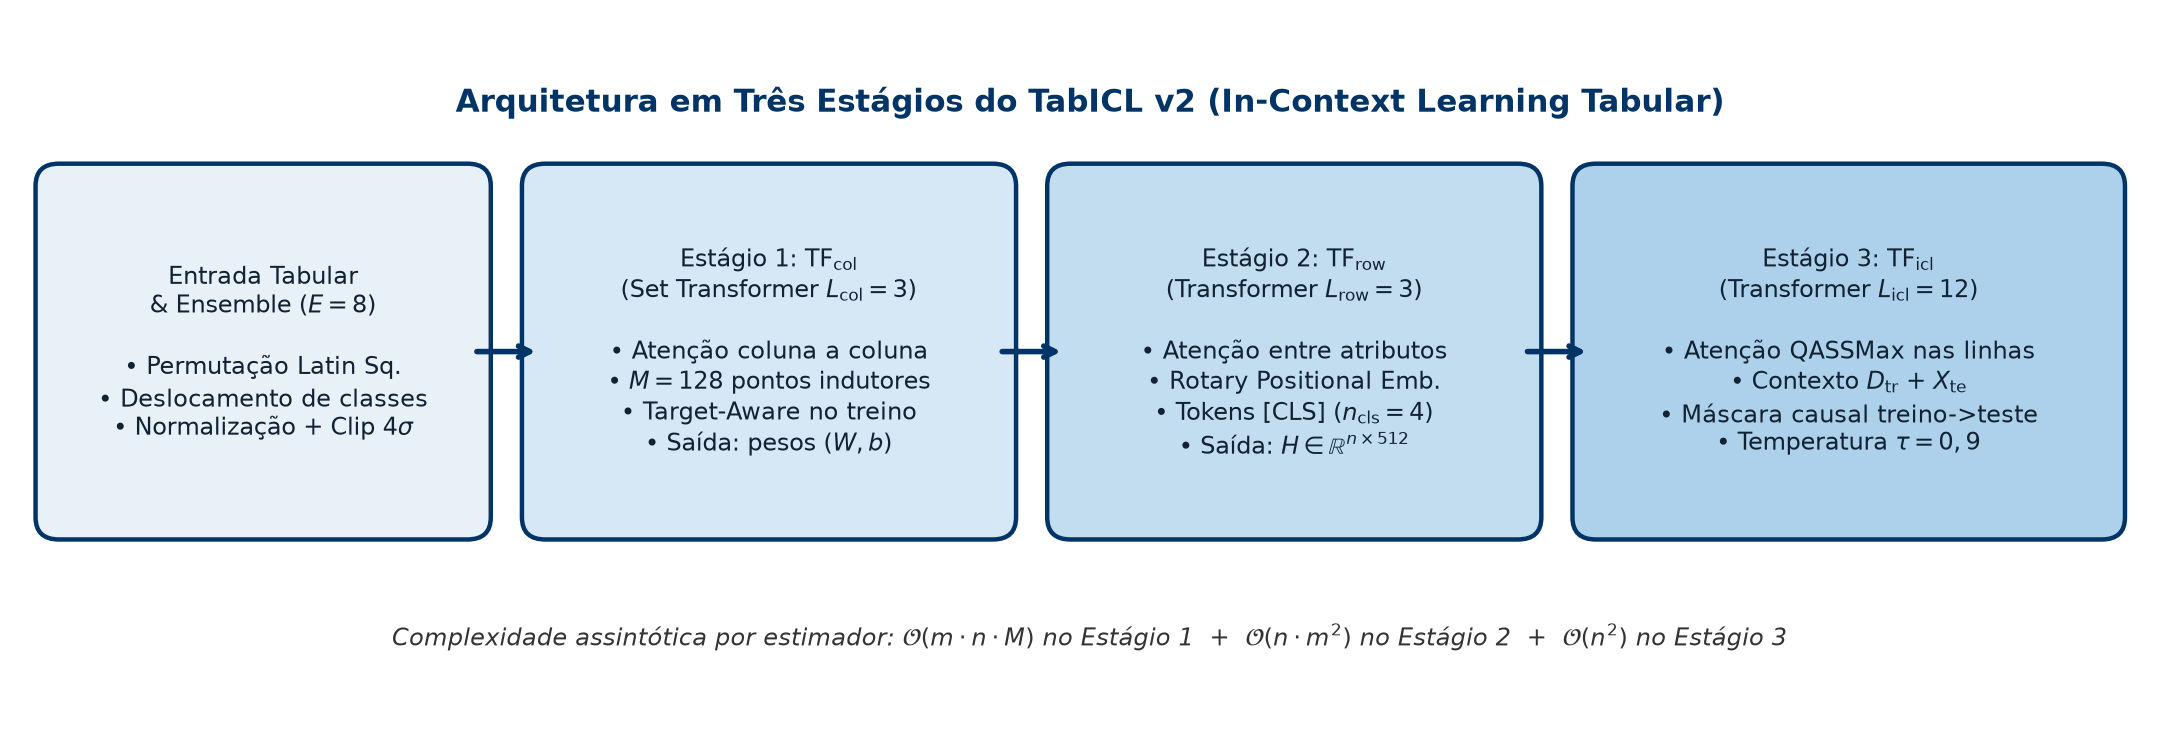
\includegraphics[width=0.98\textwidth]{../figuras/arquitetura_tabicl.png}
    \caption{Diagrama em blocos da arquitetura em três estágios do TabICL v2: pré-processamento e geração de $E=8$ visões de ensemble, Estágio~1 ($\mathrm{TF}_{\mathrm{col}}$ para incorporação consciente da distribuição de cada coluna), Estágio~2 ($\mathrm{TF}_{\mathrm{row}}$ para interação entre atributos por linha) e Estágio~3 ($\mathrm{TF}_{\mathrm{icl}}$ para aprendizagem em contexto entre amostras com atenção QASSMax).}
    \label{fig:arquitetura_tabicl}
\end{figure}

\paragraph{Estágio 1: Incorporação coluna a coluna consciente da distribuição ($\mathrm{TF}_{\mathrm{col}}$).}
Diferentemente de redes tabulares convencionais que projetam cada célula $x_{i,j}$ por uma camada linear fixa ou independente das demais linhas, o TabICL processa cada coluna $x_{:,j} \in \mathbb{R}^n$ individualmente por meio de um \emph{Set Transformer} \cite{lee2019set} compartilhado entre todas as $m$ colunas, composto por $L_{\mathrm{col}} = 3$ blocos de atenção induzida com dimensão oculta $d_{\mathrm{col}} = 128$, $h_{\mathrm{col}} = 4$ cabeças de atenção e $M = 128$ vetores indutores aprendíveis $I \in \mathbb{R}^{M \times d_{\mathrm{col}}}$.

No TabICL v2, duas inovações estruturais antecedem a atenção induzida:
\begin{enumerate}[leftmargin=2em]
    \item \textbf{Agrupamento de atributos repetidos (\emph{Repeated Feature Grouping}):} quando o conjunto de dados possui $m > d_{\mathrm{col}}$ colunas, atributos com valores idênticos são agrupados e colunas correlacionadas ou excedentes são projetadas conjuntamente em grupos de até $K_{\max} = 15$ atributos por canal por meio de camadas lineares aprendíveis $W_k \in \mathbb{R}^{k \times d_{\mathrm{col}}}$, reduzindo o custo computacional em bases de alta dimensionalidade;
    \item \textbf{Incorporação precoce consciente do alvo (\emph{Early Target-Aware Embedding}):} para permitir que o Estágio~1 capture dependências diretas entre cada atributo e a variável resposta sem vazar rótulos de teste, as células das amostras de treinamento recebem uma soma aditiva da projeção linear do atributo com a incorporação one-hot do rótulo de treino $y_i$:
    \begin{equation}
        u_{i,j}^{(0)} =
        \begin{cases}
            v_{\mathrm{feat}}(x_{i,j}) + E_y(y_i), & \text{se } 1 \le i \le n_{\mathrm{tr}}, \\
            v_{\mathrm{feat}}(x_{i,j}), & \text{se } n_{\mathrm{tr}} < i \le n.
        \end{cases}
        \label{eq:target_aware_col}
    \end{equation}
\end{enumerate}

Para evitar vazamento da distribuição das instâncias de teste para as representações das amostras de treinamento, o bloco de atenção induzida (\emph{Induced Self-Attention Block}, ISAB) restringe as chaves e valores consultados pelos pontos indutores $I$ exclusivamente às $n_{\mathrm{tr}}$ amostras de treinamento:
\begin{align}
    Z_j &= \mathrm{MHA}\!\left(Q = I, \; K = U_{\mathrm{tr}, j}, \; V = U_{\mathrm{tr}, j}\right) \in \mathbb{R}^{M \times d_{\mathrm{col}}}, \label{eq:isab_train} \\
    \tilde{U}_j &= \mathrm{MHA}\!\left(Q = U_j, \; K = Z_j, \; V = Z_j\right) \in \mathbb{R}^{n \times d_{\mathrm{col}}}, \label{eq:isab_all}
\end{align}
em que $U_{\mathrm{tr}, j} \in \mathbb{R}^{n_{\mathrm{tr}} \times d_{\mathrm{col}}}$ contém apenas as linhas de treinamento da coluna $j$, e $U_j \in \mathbb{R}^{n \times d_{\mathrm{col}}}$ contém todas as $n$ linhas. Ao final dos $L_{\mathrm{col}} = 3$ blocos, duas redes de projeção mapeiam $\tilde{U}_j$ em matrizes de pesos adaptativos $W \in \mathbb{R}^{n \times m \times d_{\mathrm{col}}}$ e vieses $b \in \mathbb{R}^{n \times m \times d_{\mathrm{col}}}$, gerando a incorporação contextualizada de cada célula por transformação afim:
\begin{equation}
    E_{i,j} = x_{i,j} \, W_{i,j,:} + b_{i,j,:} \in \mathbb{R}^{d_{\mathrm{col}}}.
    \label{eq:affine_cell}
\end{equation}
A Equação~\eqref{eq:affine_cell} confere ao $\mathrm{TF}_{\mathrm{col}}$ a capacidade de extrair estatísticas de ordem superior da distribuição empírica de cada coluna (como assimetria, multimodalidade, quantis e correlação marginal com $y_{\mathrm{tr}}$), atribuindo semântica específica a cada atributo antes mesmo de cruzá-lo com outras colunas.

\paragraph{Estágio 2: Interação entre atributos por linha ($\mathrm{TF}_{\mathrm{row}}$).}
Para cada instância $i \in \{1, \dots, n\}$, a sequência de $m$ vetores de atributos $(E_{i,1}, \dots, E_{i,m}) \in \mathbb{R}^{m \times d_{\mathrm{col}}}$ é precedida por $n_{\mathrm{cls}} = 4$ tokens especiais aprendíveis de agregação $[\mathrm{CLS}]_1, \dots, [\mathrm{CLS}]_4 \in \mathbb{R}^{d_{\mathrm{col}}}$, formando uma sequência de comprimento $m + 4$. Essa sequência é processada por um Transformer $\mathrm{TF}_{\mathrm{row}}$ de $L_{\mathrm{row}} = 3$ camadas e $h_{\mathrm{row}} = 8$ cabeças de atenção com codificação posicional rotacional multidimensional (\emph{Rotary Position Embedding}, RoPE). O uso de RoPE rompe a simetria estrita de permutação apenas após a ordenação pseudoaleatória controlada pelo ensemble (quadrados latinos), permitindo que cabeças distintas de atenção distingam colunas de valores numéricos idênticos. Ao final da terceira camada, as saídas correspondentes aos $n_{\mathrm{cls}} = 4$ tokens $[\mathrm{CLS}]$ são concatenadas, formando a representação vetorial compacta da instância $i$:
\begin{equation}
    h_i = \mathrm{Concat}\!\left(\mathrm{TF}_{\mathrm{row}}([\mathrm{CLS}]_{1:4}, E_{i,1:m})_{1:4}\right) \in \mathbb{R}^{d_{\mathrm{icl}}}, \qquad d_{\mathrm{icl}} = n_{\mathrm{cls}} \cdot d_{\mathrm{col}} = 4 \times 128 = 512.
    \label{eq:tf_row}
\end{equation}

\paragraph{Estágio 3: Aprendizagem em contexto sobre instâncias ($\mathrm{TF}_{\mathrm{icl}}$) e atenção QASSMax.}
No terceiro estágio, cada linha da tabela já está representada por um único vetor $h_i \in \mathbb{R}^{512}$ independente do número original de colunas $m$. Para condicionar o contexto nos rótulos de treinamento novamente no espaço de representação das linhas, adiciona-se a codificação one-hot projetada do rótulo $y_i$ exclusivamente às instâncias de treinamento:
\begin{equation}
    z_i^{(0)} =
    \begin{cases}
        h_i + W_y \, \mathrm{OneHot}(y_i), & \text{se } 1 \le i \le n_{\mathrm{tr}}, \\
        h_i, & \text{se } n_{\mathrm{tr}} < i \le n.
    \end{cases}
    \label{eq:icl_input}
\end{equation}
A sequência completa $Z^{(0)} = [z_1^{(0)}, \dots, z_n^{(0)}]^\top \in \mathbb{R}^{n \times 512}$ atravessa então um Transformer profundo de $L_{\mathrm{icl}} = 12$ camadas com $h_{\mathrm{icl}} = 4$ cabeças de atenção ($\mathrm{TF}_{\mathrm{icl}}$), sem codificação posicional (garantindo invariância exata à permutação das amostras de treinamento). A máscara de atenção do $\mathrm{TF}_{\mathrm{icl}}$ permite que as amostras de treinamento atendam entre si livremente ($1 \le i, i' \le n_{\mathrm{tr}}$) e que cada amostra de teste ($i > n_{\mathrm{tr}}$) atenda exclusivamente às amostras de treinamento ($1 \le i' \le n_{\mathrm{tr}}$), nunca a si mesma ou a outras amostras de teste. Dessa forma, a predição para cada ponto de teste depende unicamente do contexto de treinamento $\mathcal{D}_{\mathrm{tr}}$ e de seus próprios atributos $x_i$.

Um problema crítico de Transformers de contexto longo é o desvanecimento de atenção (\emph{attention fading}): quando $n_{\mathrm{tr}}$ cresce de centenas durante o pré-treinamento para dezenas de milhares na inferência, o denominador da função softmax dilui os pesos de atenção. Para corrigir esse fenômeno, o TabICL v2 substitui a atenção padrão no Estágio~3 (e no Estágio~1) pela \textbf{QASSMax} (\emph{Query-Aware Scalable Softmax}), que escala os logits de atenção por uma função logarítmica modulada por um portão dependente da consulta $q \in \mathbb{R}^{d_h}$:
\begin{align}
    s_{\mathrm{base}}(n_{\mathrm{ctx}}) &= 1 + \mathrm{softplus}(\alpha) \log(n_{\mathrm{ctx}}), \label{eq:qassmax_base} \\
    g(q) &= 1 + \tanh(\mathrm{MLP}(q)), \label{eq:qassmax_gate} \\
    \tilde{q} &= q \cdot s_{\mathrm{base}}(n_{\mathrm{ctx}}) \odot g(q), \label{eq:qassmax_query}
\end{align}
em que $n_{\mathrm{ctx}} = n_{\mathrm{tr}}$ é o tamanho do contexto atendido, $\alpha \in \mathbb{R}$ é um escalar aprendível por cabeça e $\mathrm{MLP}(q)$ é um perceptron de duas camadas ($d_h \to d_h/2 \to 1$). Essa formulação permite que cabeças que realizam agregação global mantenham distribuição uniforme enquanto cabeças seletivas (como busca de vizinhos mais próximos no contexto) concentrem massa de probabilidade mesmo quando $n_{\mathrm{tr}} \gg 10.000$.

Finalmente, a representação da última camada $z_i^{(12)} \in \mathbb{R}^{512}$ de cada instância de teste $i > n_{\mathrm{tr}}$ passa por uma cabeça linear de saída $W_{\mathrm{out}} \in \mathbb{R}^{C_{\max} \times 512}$ truncada às $C$ classes ativas da tarefa e calibrada pela temperatura de softmax $\tau > 0$:
\begin{equation}
    \hat{p}_e(y_i = c \mid x_i, \mathcal{D}_{\mathrm{tr}}) = \frac{\exp\!\left(\ell_{i,c}^{(e)} / \tau\right)}{\sum_{c'=1}^{C} \exp\!\left(\ell_{i,c'}^{(e)} / \tau\right)}, \qquad \ell_i^{(e)} = \left(W_{\mathrm{out}} z_i^{(12)} + b_{\mathrm{out}}\right)_{1:C}.
    \label{eq:softmax_temp}
\end{equation}
Quando o número de classes da tarefa excede a capacidade direta do pré-treinamento ($C > 10$), o TabICL v2 aciona automaticamente a decomposição em base mista balanceada (\emph{Mixed-Radix Decomposition} / classificação hierárquica, habilitada por \texttt{support\_many\_classes=True}), fatorando o rótulo $y \in \{0, \dots, C-1\}$ em dígitos $d_r \in \{0, \dots, b_r - 1\}$ com $b_r \le 10$ e combinando as probabilidades condicionais pelo produto da regra da cadeia.

\subsection{Forma de aprendizado e representação dos padrões}
\label{sec:aprendizado}

O aprendizado do TabICL v2 divide-se em duas fases radicalmente distintas: o \textbf{pré-treinamento sintético offline} (executado uma única vez pelos autores do modelo) e a \textbf{inferência em contexto online} durante o uso em produção (fases \texttt{fit} e \texttt{predict\_proba} do estimador scikit-learn).

\paragraph{Pré-treinamento sintético e aproximação da PPD Bayesiana.}
Seguindo o arcabouço teórico das PFNs \cite{hollmann2023tabpfn,qu2025tabicl}, o objetivo do pré-treinamento é aproximar a Distribuição Preditiva Posterior (\emph{Posterior Predictive Distribution}, PPD) associada a uma distribuição a priori $p(\mathcal{T})$ sobre tarefas tabulares geradas por Modelos Causais Estruturais (SCMs) e processos gaussianos com kernels de Sobolev. Em cada iteração de pré-treinamento, amostra-se um grafo acíclico direcionado (DAG) ou estrutura em árvore/MLP, funções de mecanismo não lineares (incluindo ativações racionais de Cauchy $\phi(x) = \sum_k a_k / ((x - c_k)^2 + \gamma_k^2)$, splines quadráticas, funções periódicas e árvores de decisão aleatórias), ruídos heterocedásticos e transformações marginais de cauda pesada (Kumaraswamy e exponenciais), gerando um dataset sintético $D = \mathcal{D}_{\mathrm{tr}} \cup \mathcal{D}_{\mathrm{te}}$. Os parâmetros $\theta$ do modelo (cerca de $33\text{ milhões}$ de pesos treináveis) são otimizados pela minimização da perda esperada de entropia cruzada sobre os exemplos de teste sintéticos:
\begin{equation}
    \mathcal{L}(\theta) = \mathbb{E}_{D \sim p(\mathcal{T})} \left[ - \sum_{(x_{\mathrm{te}}, y_{\mathrm{te}}) \in \mathcal{D}_{\mathrm{te}}} \log p_\theta(y_{\mathrm{te}} \mid x_{\mathrm{te}}, \mathcal{D}_{\mathrm{tr}}) \right].
    \label{eq:ppd_loss}
\end{equation}
Minimizar a Equação~\eqref{eq:ppd_loss} equivale a minimizar a divergência de Kullback-Leibler esperada $\mathbb{E}_{\mathcal{D}_{\mathrm{tr}}, x_{\mathrm{te}}} \big[ D_{\mathrm{KL}}\big( p(y_{\mathrm{te}} \mid x_{\mathrm{te}}, \mathcal{D}_{\mathrm{tr}}) \,\|\, p_\theta(y_{\mathrm{te}} \mid x_{\mathrm{te}}, \mathcal{D}_{\mathrm{tr}}) \big) \big]$ em relação à verdadeira PPD Bayesiana induzida pelo prior sintético. O TabICL v2 foi pré-treinado por $100.000$ passos sobre aproximadamente $220\text{ milhões}$ de datasets sintéticos em três estágios de currículo de tamanho contextual (de $n \in [300, 2.048]$ até $n \in [300, 60.000]$), substituindo o otimizador AdamW pelo otimizador \textbf{Muon} (\emph{Momentum Orthogonalized by Newton-Schulz} \cite{jordan2024muon}) nas matrizes bidimensionais das camadas ocultas, combinado ao decaimento cosseno com aquecimento (\emph{warmup-stable-decay}).

\paragraph{Inferência em contexto e pipeline nativo de pré-processamento e ensemble.}
Na aplicação a um dataset real do TabArena, \textbf{nenhum gradiente é calculado e nenhum peso neural $\theta$ é atualizado}. O método \texttt{fit(X\_train, y\_train)} executa um pipeline determinístico de preparação de visões (\texttt{EnsembleGenerator}):
\begin{enumerate}[leftmargin=2em]
    \item \textbf{Codificação de rótulos e atributos:} o alvo $y_{\mathrm{tr}}$ é mapeado para inteiros contíguos via \texttt{LabelEncoder}; colunas categóricas, booleanas ou textuais são convertidas em códigos ordinais inteiros via \texttt{OrdinalEncoder} com tratamento explícito de categorias desconhecidas no teste, e atributos constantes são descartados;
    \item \textbf{Geração de $E = n\_estimators$ visões de ensemble:} como os estágios $\mathrm{TF}_{\mathrm{row}}$ (com RoPE) e a cabeça de saída possuem leve sensibilidade à ordem das colunas e dos índices das classes, o modelo constrói $E = 8$ transformações distintas dos dados de entrada. Os métodos de normalização declarados em \texttt{norm\_methods} (por padrão \texttt{["none", "power"]}, que aplica identidade a metade dos estimadores e transformação de potência Yeo-Johnson padronizada à outra metade) são distribuídos ciclicamente entre as $E$ visões;
    \item \textbf{Imputação, normalização e truncamento de valores extremos:} dentro de cada visão $e \in \{1, \dots, E\}$, valores ausentes (\texttt{NaN}) em colunas numéricas são imputados pela mediana calculada exclusivamente sobre $X_{\mathrm{tr}}$. Após a normalização escolhida para a visão $e$, aplica-se o truncamento simétrico de outliers controlando caudas extremas pelo limiar $\tau_{\mathrm{out}} = \texttt{outlier\_threshold}$ (padrão $4{,}0$ desvios-padrão), seguido de re-padronização para média zero e variância unitária:
    \begin{equation}
        \tilde{x}_{i,j} = \mathrm{clip}\!\left(\hat{x}_{i,j}, \; -\tau_{\mathrm{out}}, \; +\tau_{\mathrm{out}}\right);
        \label{eq:outlier_clip}
    \end{equation}
    \item \textbf{Permutação por quadrados latinos e deslocamento cíclico de classes:} para garantir cobertura balanceada de ordens de colunas com poucos estimadores, as $E$ permutações de atributos são amostradas via quadrados latinos (\texttt{feat\_shuffle\_method="latin"}) e os índices das classes sofrem deslocamentos cíclicos (\texttt{class\_shuffle\_method="shift"}).
\end{enumerate}
No método \texttt{predict\_proba(X\_test)}, cada uma das $E$ visões atravessa os três estágios ($\mathrm{TF}_{\mathrm{col}} \to \mathrm{TF}_{\mathrm{row}} \to \mathrm{TF}_{\mathrm{icl}}$), as permutações de classe são desfeitas e as predições dos $E$ estimadores são combinadas por média aritmética dos logits antes da softmax calibrada por $\tau$ (quando \texttt{average\_logits=True}) ou por média das probabilidades após a softmax (quando \texttt{average\_logits=False}).

\subsection{Complexidade computacional}
\label{sec:complexidade}

Seja $n = n_{\mathrm{tr}} + n_{\mathrm{te}}$ o número total de amostras (contexto de treinamento mais lote de teste), $m$ o número de atributos, $M = 128$ o número de pontos indutores do \emph{Set Transformer}, $E$ o número de estimadores do ensemble e $d_{\mathrm{col}} = 128$, $d_{\mathrm{icl}} = 512$ as dimensões ocultas fixas da arquitetura.

\paragraph{Complexidade de tempo.}
Em contraste com os modelos baseados em árvores (GBDTs), nos quais o custo concentra-se em \texttt{fit()} com $\mathcal{O}(T \cdot m \cdot n_{\mathrm{tr}} \log n_{\mathrm{tr}})$ (ou $\mathcal{O}(T \cdot m \cdot n_{\mathrm{tr}})$ com histogramas de $B$ bins no LightGBM) e a inferência é rápida em $\mathcal{O}(T \cdot D_{\max} \cdot n_{\mathrm{te}})$, o TabICL v2 transfere a quase totalidade do trabalho computacional dos Transformers para o momento da inferência contextual (ou pré-computação das representações de treino):
\begin{itemize}[leftmargin=2em]
    \item \textbf{Fase \texttt{fit()}:} ajusta apenas as transformações estatísticas leves das $E$ visões (codificação ordinal, medianas, transformações Yeo-Johnson ou quantílicas e permutações latinas), demandando tempo $\mathcal{O}(E \cdot n_{\mathrm{tr}} \cdot m)$ em CPU;
    \item \textbf{Fase \texttt{predict\_proba()} (passagem pelos três estágios por estimador):}
    \begin{enumerate}
        \item No \textbf{Estágio 1 ($\mathrm{TF}_{\mathrm{col}}$)}, cada uma das $m$ colunas aplica atenção induzida entre $n$ amostras e $M$ pontos indutores ao longo de $L_{\mathrm{col}}$ blocos, custando $\mathcal{O}(L_{\mathrm{col}} \cdot m \cdot n \cdot M \cdot d_{\mathrm{col}}) = \mathcal{O}(n \cdot m)$ operações (linear em $n$ e em $m$, pois $M = 128$ é constante);
        \item No \textbf{Estágio 2 ($\mathrm{TF}_{\mathrm{row}}$)}, para cada uma das $n$ linhas, calcula-se autoatenção quadrática sobre a sequência de $m + n_{\mathrm{cls}}$ tokens ao longo de $L_{\mathrm{row}}$ camadas, custando $\mathcal{O}(L_{\mathrm{row}} \cdot n \cdot m^2 \cdot d_{\mathrm{col}}) = \mathcal{O}(n \cdot m^2)$;
        \item No \textbf{Estágio 3 ($\mathrm{TF}_{\mathrm{icl}}$)}, calcula-se atenção sobre os $n$ vetores de linha compactados de dimensão $d_{\mathrm{icl}} = 512$ ao longo de $L_{\mathrm{icl}} = 12$ camadas (independente de $m$), custando $\mathcal{O}(L_{\mathrm{icl}} \cdot (n_{\mathrm{tr}}^2 + n_{\mathrm{te}} \cdot n_{\mathrm{tr}}) \cdot d_{\mathrm{icl}}) = \mathcal{O}(n^2)$.
    \end{enumerate}
\end{itemize}
Somando os três estágios para os $E$ estimadores do ensemble, a complexidade assintótica total de tempo de inferência do TabICL v2 é:
\begin{equation}
    \mathcal{T}_{\mathrm{TabICL}}(n, m, E) = \mathcal{O}\!\left(E \cdot \left(n \cdot m \cdot M + n \cdot m^2 + n^2\right)\right) = \mathcal{O}\!\left(E \cdot (n m^2 + n^2)\right).
    \label{eq:time_complexity}
\end{equation}
Comparado ao TabPFN v2, cuja atenção bidimensional acoplada exige $\mathcal{O}(n^2 m + n m^2)$, o TabICL v2 elimina o fator multiplicativo $m$ do termo quadrático $n^2$.

\paragraph{Complexidade de memória e gerenciamento em alta dimensionalidade.}
O tensor intermediário mais volumoso da arquitetura é a representação celular $E \in \mathbb{R}^{B_{\mathrm{batch}} \times n \times m \times d_{\mathrm{col}}}$ na transição entre $\mathrm{TF}_{\mathrm{col}}$ e $\mathrm{TF}_{\mathrm{row}}$, exigindo espaço $\mathcal{O}(n \cdot m \cdot d_{\mathrm{col}})$, enquanto as matrizes de atenção do $\mathrm{TF}_{\mathrm{row}}$ e do $\mathrm{TF}_{\mathrm{icl}}$ exigem $\mathcal{O}(n \cdot m^2)$ e $\mathcal{O}(n^2)$, respectivamente (reduzidos na prática pelo uso de kernels \emph{FlashAttention} / \texttt{scaled\_dot\_product\_attention} do PyTorch em meia precisão \texttt{float16}). Em bases com número muito elevado de atributos ($m > 500$, como \texttt{Bioresponse} com $m = 1.776$ e \texttt{hiva\_agnostic} com $m = 1.617$), o tensor $(n \times m \times d_{\mathrm{col}})$ pode exceder os $15\text{ GiB}$ de VRAM de uma GPU NVIDIA Tesla T4 ou a memória paginada da CPU se múltiplas colunas forem processadas em lotes grandes. Por esse motivo, a biblioteca \texttt{tabicl} implementa execução em lotes adaptativos de colunas/linhas e suporte a descarregamento em disco (\texttt{disk\_offload\_dir}), mecanismo ativado automaticamente pelo nosso wrapper \texttt{AdaptiveTabICLClassifier} quando $m > 500$.

\subsection{Posicionamento na literatura}
\label{sec:literatura}

O posicionamento do TabICL v2 na literatura recente de Aprendizagem de Máquina tabular (2023--2026) situa-se na convergência de três linhas de pesquisa:
\begin{enumerate}[leftmargin=2em]
    \item \textbf{Aproximação de GBDTs tunados e ensembles neurais paramétricos:} Holzmüller, Grinsztajn e Steinwart \cite{holzmuller2024better} demonstraram no NeurIPS 2024 que configurações padrão cuidadosamente meta-otimizadas para GBDTs (\emph{Tuned Defaults} no pacote \texttt{pytabkit}) fecham grande parte da lacuna entre modelos padrão e modelos ajustados por busca cara, servindo de referência forte na literatura e no presente projeto. Paralelamente, Gorishniy et al. propuseram o TabR \cite{gorishniy2024tabr} (ICLR 2024), que incorpora um módulo de atenção estilo $k$-vizinhos mais próximos sobre o conjunto de treino dentro de uma rede treinada por gradiente, e o TabM \cite{gorishniy2025tabm} (ICLR 2025), que constrói ensembles eficientes de MLPs compartilhando pesos via adaptadores de posto 1 (\emph{BatchEnsemble});
    \item \textbf{Evolução dos modelos fundacionais de aprendizagem em contexto (PFNs):} Hollmann et al. publicaram a versão fundacional do TabPFN \cite{hollmann2023tabpfn} (ICLR 2023, restrita a $n \le 1.000$ e $m \le 100$) e posteriormente o TabPFN v2 \cite{hollmann2025tabpfn} na revista \emph{Nature} (2025), demonstrando superioridade sobre GBDTs tunados em bases pequenas e médias de até $10.000$ amostras. Contudo, o custo $\mathcal{O}(n^2 m + n m^2)$ do TabPFN v2 motivou Qu et al. \cite{qu2025tabicl} (ICML 2025) a introduzirem a arquitetura desacoplada coluna-depois-linha do TabICL v1;
    \item \textbf{Consolidação em benchmarks de larga escala (TabArena e TabICL v2):} em 2025, Erickson et al. \cite{erickson2025tabarena} lançaram o benchmark vivo \textbf{TabArena}, curando datasets tabulares reais com splits padronizados e protocolos de validação aninhada. Em fevereiro de 2026, Qu et al. \cite{qu2026tabiclv2} apresentaram o \textbf{TabICL v2}, redesenhando o gerador sintético (funções de Cauchy, kernels de Sobolev, amostragem Kumaraswamy), introduzindo a atenção QASSMax e o otimizador Muon, e demonstrando que o TabICL v2 supera tanto o TabPFN v2 quanto o TabPFN-2.5 nos benchmarks TabArena e TALENT sem requerer ajuste de hiperparâmetros, operando com velocidade de inferência uma ordem de grandeza superior em tabelas largas.
\end{enumerate}

\subsection{Hiperparâmetros principais e espaço de busca}
\label{sec:hiperparametros}

Como o TabICL v2 realiza inferência em contexto com pesos neurais congelados, seus hiperparâmetros expostos ao usuário controlam a diversidade das visões do ensemble de entrada, o tratamento estatístico de valores discrepantes e escalas marginais, a agregação entre estimadores e a forma da distribuição preditiva. A Tabela~\ref{tab:hiperparametros} resume todos os hiperparâmetros relevantes do modelo, seus papéis estruturais, a configuração padrão adotada em \texttt{group\_default} e o espaço de busca Bayesiana declarado a priori para \texttt{group\_tuned}.

\begin{table}[htbp]
    \centering
    \caption{Hiperparâmetros do modelo tema TabICL v2 (\texttt{AdaptiveTabICLClassifier}), configuração padrão adotada (\texttt{group\_default}) e espaço de busca declarado a priori (\texttt{group\_tuned}).}
    \label{tab:hiperparametros}
    \small
    \resizebox{\textwidth}{!}{%
    \begin{tabular}{@{}llllp{4.6cm}@{}}
        \toprule
        \textbf{Hiperparâmetro} & \textbf{Tipo} & \textbf{Padrão} & \textbf{Espaço de busca} & \textbf{Papel no modelo} \\
        \midrule
        \texttt{norm\_methods} & categórico & \texttt{none+power} & 5 combinações\textsuperscript{a} & Transformações de normalização marginal aplicadas às visões do ensemble \\
        \texttt{outlier\_threshold} & contínuo (linear) & $4{,}0$ & $[2{,}5;\; 6{,}0]$ & Limiar em desvios-padrão ($\sigma$) para truncamento simétrico de outliers \\
        \texttt{softmax\_temperature} & contínuo (log) & $0{,}9$ & $[0{,}5;\; 1{,}5]$ & Temperatura $\tau$ de reescalonamento dos logits antes da softmax final \\
        \texttt{average\_logits} & categórico & \texttt{True} & $\{\texttt{True}, \texttt{False}\}$ & Agregação do ensemble por média de logits (\texttt{True}) ou probabilidades (\texttt{False}) \\
        \texttt{n\_estimators} & inteiro & $8$ & fixo em $8$\textsuperscript{b} & Número de visões sintéticas (permutações de colunas e classes) no ensemble \\
        \texttt{feat\_shuffle\_method} & categórico & \texttt{"latin"} & fixo (\texttt{"latin"}) & Estratégia de permutação de atributos por quadrados latinos \\
        \texttt{class\_shuffle\_method} & categórico & \texttt{"shift"} & fixo (\texttt{"shift"}) & Deslocamento cíclico dos índices das classes entre estimadores \\
        \texttt{support\_many\_classes} & booleano & \texttt{True} & fixo (\texttt{True}) & Ativa decomposição hierárquica de base mista quando $C > 10$ \\
        \texttt{random\_state} & inteiro & $42$ & fixo ($42$) & Semente determinística das permutações de atributos e classes \\
        \bottomrule
    \end{tabular}
    }%
    \vspace{0.3em}
    \begin{flushleft}
    \footnotesize
    \textsuperscript{a} As 5 opções categóricas de \texttt{norm\_methods} são: \texttt{"none+power"}, \texttt{"none+power+robust"}, \texttt{"none+power+quantile\_rtdl"}, \texttt{"power"} e \texttt{"quantile\_rtdl"} (convertidas em listas para a API do \texttt{TabICLClassifier}).\\
    \textsuperscript{b} \texttt{n\_estimators} foi fixado em $8$ na busca para manter a avaliação de cada trial de CV interna (3 folds) dentro do orçamento de $600\text{ s}$ por fold externo; sua variação em $\{1, 2, 4, 8, 16, 32\}$ é analisada nas curvas de validação de complexidade (Seção~\ref{sec:overfitting}).
    \end{flushleft}
\end{table}

As faixas do espaço de busca em \texttt{src/models/group\_model.py} foram justificadas a priori pelas propriedades estatísticas da inferência em contexto: (i) \texttt{norm\_methods} explora transformações robustas à mediana/IQR (\texttt{robust}) e mapeamentos quantílicos gaussianos com ruído (\texttt{quantile\_rtdl} \cite{gorishniy2021revisiting}), essenciais quando atributos possuem distribuições multimodais ou caudas pesadas; (ii) \texttt{outlier\_threshold} em $[2{,}5, 6{,}0]$ ajusta o compromisso entre proteger os mecanismos de atenção de valores extremos espúrios ($\tau_{\mathrm{out}} \approx 2{,}5$) e preservar sinal informativo na cauda da distribuição ($\tau_{\mathrm{out}} \approx 6{,}0$); (iii) \texttt{softmax\_temperature} em $[0{,}5, 1{,}5]$ (escala logarítmica) ajusta a nitidez da distribuição preditiva, impactando a entropia cruzada e a ordenação multiclasse OvO; e (iv) \texttt{average\_logits} alterna entre combinação em log-probabilidades (produto geométrico normalizado de especialistas) e mistura linear de probabilidades.

\subsection{Aplicações práticas e limitações}
\label{sec:limitacoes}

\paragraph{Cenários em que o TabICL v2 é particularmente indicado.}
O TabICL v2 constitui uma alternativa relevante a avaliar em problemas de classificação tabular de pequeno e médio porte ($n \le 10.000$ amostras) e tabelas com número moderado de atributos ($m \le 200$), nos quais sua inferência Bayesiana amortizada extrai relações multivariadas complexas sem atualizar seus pesos pré-treinados por descida de gradiente durante o ajuste da tarefa. Além disso, por não exigir ajuste de hiperparâmetros para alcançar desempenho competitivo e produzir menores valores de entropia cruzada no conjunto de testes deste estudo, pode ser vantajoso em fluxos de prototipagem rápida, sistemas médicos, financeiros ou industriais com dados escassos e pipelines automatizados (\emph{zero-shot tabular learning}).

\paragraph{Limitações teóricas e práticas.}
Apesar de seus pontos fortes, o modelo apresenta limitações importantes que devem ser consideradas:
\begin{enumerate}[leftmargin=2em]
    \item \textbf{Dependência de aceleradores gráficos (GPU) e latência de inferência:} enquanto GBDTs treinados realizam predições em poucos milissegundos na CPU, cada chamada a \texttt{predict\_proba} no TabICL v2 executa $E = 8$ passagens por dois Transformers de 3 camadas e um Transformer de 12 camadas sobre todo o contexto de treino, demandando segundos por lote mesmo em GPU;
    \item \textbf{Escala quadrática em amostras ($\mathcal{O}(n^2)$) e atributos ($\mathcal{O}(n m^2)$):} quando o conjunto de treinamento ultrapassa dezenas de milhares de instâncias ou centenas de atributos ($m > 500$), o consumo de memória VRAM cresce rapidamente, exigindo subamostragem do contexto ou descarregamento para disco (\emph{disk offloading}), o que eleva o tempo de execução;
    \item \textbf{Dependência de pré-processamento tabular para variáveis textuais livres ou séries temporais puras:} o modelo assume que as colunas podem ser representadas como grandezas numéricas ou categorias ordinais/discretas, não substituindo codificadores de texto livre ou modelos autorregressivos temporais dedicados.
\end{enumerate}

% =============================================================================
\section{Etapa 2: Estudo experimental}
\label{sec:etapa2}

\subsection{Seleção dos datasets}
\label{sec:selecao}

A suíte oficial \textbf{TabArena-v0.1} (OpenML, suíte 457 \cite{erickson2025tabarena}) contém 38 tarefas de classificação supervisionada tabular, divididas pelo protocolo da disciplina em três regimes de tamanho segundo o número total de amostras $n$: \textbf{pequeno} ($n < 2.500$, 12 tarefas disponíveis), \textbf{médio} ($2.500 \le n < 10.000$, exatamente 10 tarefas disponíveis) e \textbf{grande} ($n \ge 10.000$, 16 tarefas disponíveis). A seleção do grupo foi fixada em \texttt{data/selecao\_datasets.txt} (validada sem avisos por \texttt{python -m src.pipeline.check\_selection}) com exatamente 30 datasets: 10 pequenos, 10 médios e 10 grandes.

Os critérios objetivos que guiaram a escolha nos regimes com folga de catálogo foram:
\begin{enumerate}[leftmargin=2em]
    \item \textbf{Regime pequeno (10 selecionados dentre 12):} foram excluídas as tarefas \texttt{363678} (\texttt{MIC}, $n = 1.699$, $m = 111$, com alta esparsidade de valores ausentes e 91,9\% de atributos categóricos) e \texttt{363711} (\texttt{anneal}, $n = 898$, $m = 38$, 5 classes fortemente desbalanceadas com razão $85{,}50$). As 10 bases mantidas cobrem $n \in [748, 2.400]$, $m \in [4, 41]$, problemas binários (8 bases) e multiclasse (2 bases: \texttt{maternal\_health\_risk} e \texttt{website\_phishing}), ambos os regimes de proporção categórica e presença de dados ausentes (\texttt{Fitness\_Club} e \texttt{Marketing\_Campaign});
    \item \textbf{Regime médio (10 selecionados dentre 10):} como o catálogo possui exatamente 10 tarefas neste intervalo, todas foram obrigatoriamente incluídas, abrangendo desde problemas densos de baixa dimensão até desafios extremos de alta dimensionalidade (\texttt{Bioresponse} com $m = 1.776$ e \texttt{hiva\_agnostic} com $m = 1.617$ e razão de desbalanceamento $88{,}33$) e 3 problemas multiclasse (\texttt{splice}, \texttt{hiva\_agnostic} e \texttt{students\_dropout\_and\_academic\_success});
    \item \textbf{Regime grande (10 selecionados dentre 16):} como o método \texttt{final\_test} subamostra estratificadamente o treinamento externo em no máximo $10.000$ instâncias, priorizaram-se as bases com $n$ mais próximo desse limiar efetivo ($10.459 \le n \le 45.211$), preservando adicionalmente o único dataset multiclasse grande da suíte (\texttt{363699} \texttt{SDSS17}, $n = 78.053$, 3 classes) e uma base massiva com dados ausentes e alta fração categórica (\texttt{363628} \texttt{customer\_satisfaction\_in\_airline}, $n = 129.880$). Foram excluídas 6 tarefas binárias redundantes ou com dimensionalidade extrema (\texttt{Bank\_Customer\_Churn}, \texttt{kddcup09\_appetency} com $m = 212$, \texttt{APSFailure} com $m = 170$, \texttt{Amazon\_employee\_access}, \texttt{Diabetes130US} e \texttt{GiveMeSomeCredit}).
\end{enumerate}

No cômputo global dos 30 datasets selecionados, obtém-se equilíbrio nos quatro eixos de regime: \textbf{tamanho} (10 pequenos, 10 médios, 10 grandes), \textbf{tipo de problema} (24 binários e 6 multiclasse, garantindo ao menos um multiclasse por regime de tamanho), \textbf{proporção de atributos categóricos} (exatamente 15 datasets com $\texttt{cat\_share} < 25\%$ e 15 com $\texttt{cat\_share} \ge 25\%$) e \textbf{valores ausentes} (24 completos e 6 com dados faltantes, sendo 2 em cada regime de tamanho). A tabela completa dos 30 datasets encontra-se no Apêndice~\ref{app:datasets}.

Para os estudos diagnósticos da fase de desenvolvimento (sensibilidade, ablação, curvas de validação de complexidade e erros por classe), declarou-se a priori um subconjunto de três datasets representativos (um por regime de tamanho, avaliados exclusivamente no treino do fold externo 0): \texttt{363621} (\texttt{blood-transfusion-service-center}, pequeno, binário), \texttt{363704} (\texttt{students\_dropout\_and\_academic\_success}, médio, multiclasse de 3 classes, substituto documentado em \texttt{docs/declaracoes\_a\_priori.md} no commit \texttt{e2c6968} antes do congelamento para garantir cobertura multiclasse nos estudos de erro por classe) e \texttt{363628} (\texttt{customer\_satisfaction\_in\_airline}, grande, binário com dados ausentes e 76,2\% de atributos categóricos).

\subsection{Protocolo experimental: treino, validação e teste}
\label{sec:protocolo}

O protocolo experimental segue rigorosamente a estrutura de validação cruzada aninhada ilustrada na Figura~\ref{fig:fluxo_protocolo} e parametrizada na Tabela~\ref{tab:protocolo}. Para cada um dos 30 datasets, utilizam-se os 3 folds externos estratificados oficiais da suíte TabArena (\texttt{repeat=0, fold=0..2}). Em cada fold externo, cerca de $2/3$ das instâncias compõem o conjunto de treinamento externo e $1/3$ compõe o conjunto de teste externo selado.

\begin{figure}[htbp]
    \centering
    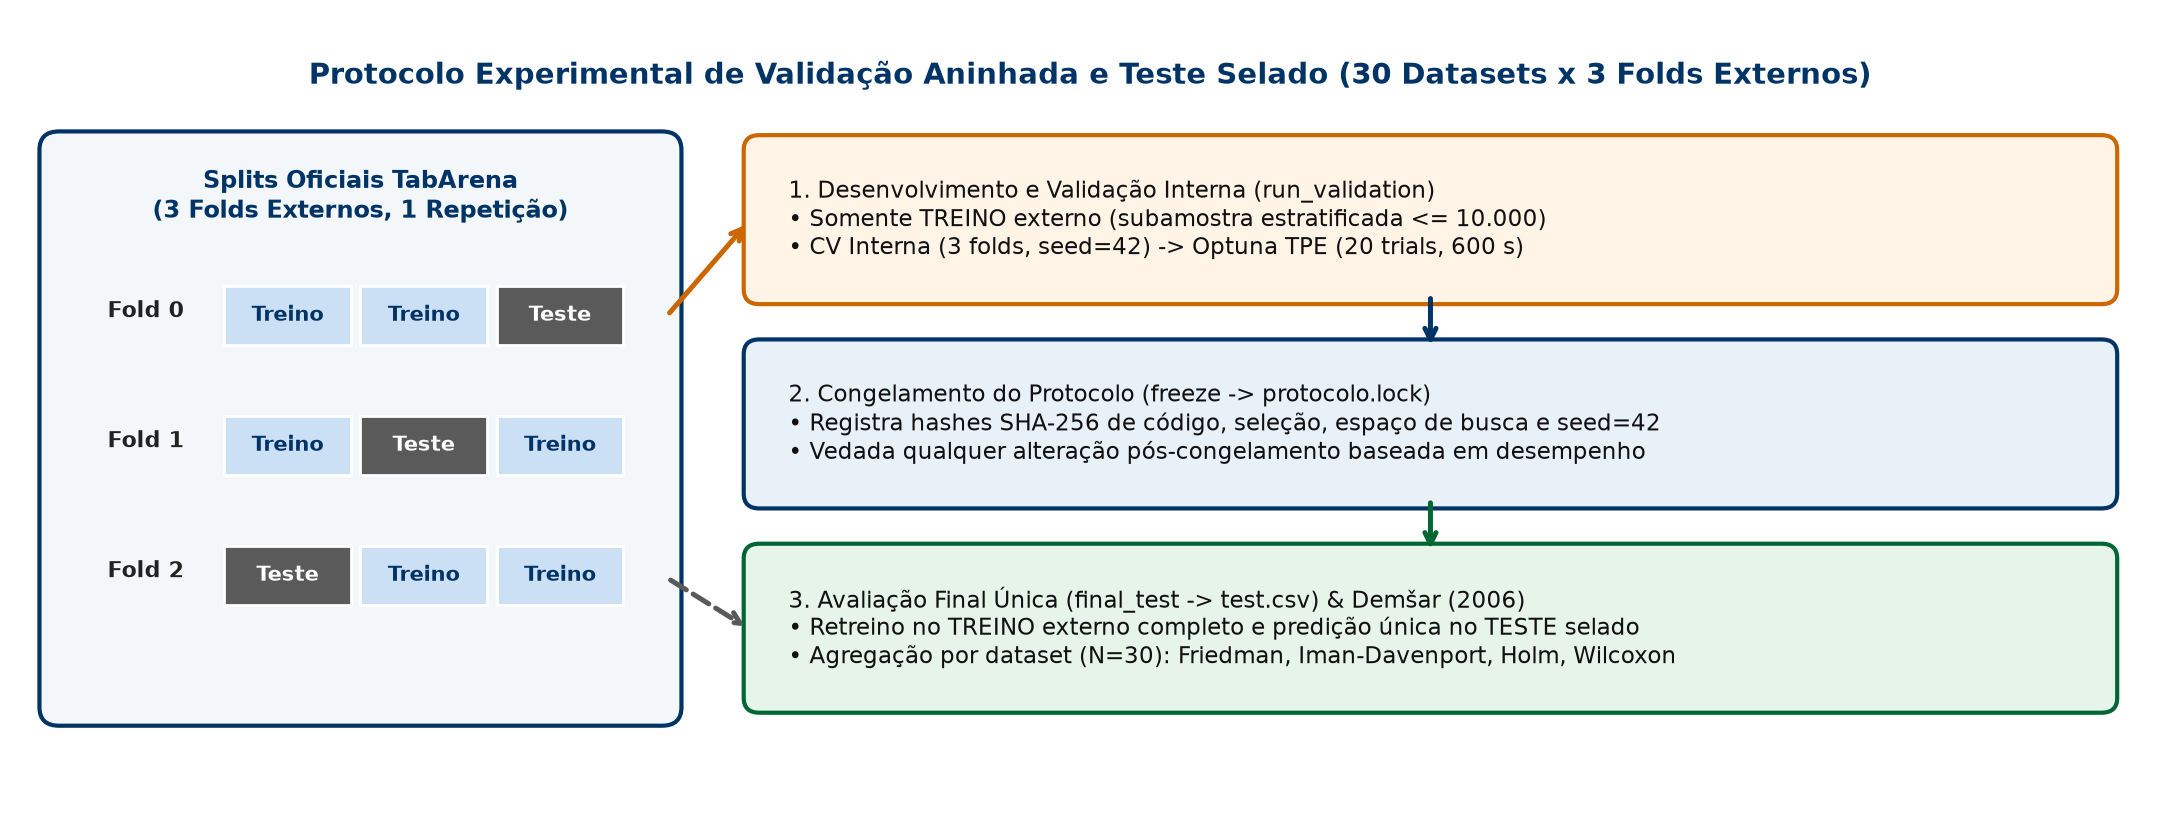
\includegraphics[width=0.98\textwidth]{../figuras/fluxo_protocolo.png}
    \caption{Fluxo do protocolo experimental em três fases: (1) desenvolvimento e validação interna exclusivamente sobre o treino dos folds externos; (2) congelamento do protocolo (\texttt{protocolo.lock}); e (3) avaliação final única no conjunto de teste externo selado seguida de análise estatística de Demšar (2006).}
    \label{fig:fluxo_protocolo}
\end{figure}

Durante toda a fase de desenvolvimento (\texttt{run\_validation.py} e notebooks 02, 03 e 05), apenas os índices de treinamento de cada fold externo (\texttt{get\_train\_indices}) são acessados. Quando o treinamento externo possui mais de $10.000$ amostras, aplica-se subamostragem estratificada determinística (\texttt{MAX\_SAMPLES = 10\_000}, \texttt{seed = 42}). Esse conjunto de treinamento externo é dividido em 3 partições internas estratificadas (\texttt{inner\_cv\_splits}, \texttt{seed = 42}). Para o sistema com busca (\texttt{group\_tuned}), o amostrador Bayesiano TPE (\emph{Tree-structured Parzen Estimator}) do Optuna executa até $20$ trials (com limite de $600\text{ s}$ por fold externo) maximizando a AUC OvO média nas 3 partições internas.

\begin{table}[htbp]
    \centering
    \caption{Parâmetros do protocolo experimental e registros de congelamento e execução.}
    \label{tab:protocolo}
    \small
    \begin{tabular}{@{}ll@{}}
        \toprule
        \textbf{Item do protocolo} & \textbf{Valor / Registro no repositório} \\
        \midrule
        Folds externos (TabArena oficial) & 3 (\texttt{repeat=0, fold=0..2}) \\
        Folds internos (busca e validação) & 3 (\texttt{StratifiedKFold}, \texttt{seed=42}) \\
        Orçamento da busca Optuna (TPE) & 20 trials, \texttt{timeout=600 s} por fold externo \\
        Teto de amostras de treino & $10.000$ (\texttt{stratified\_subsample}, \texttt{seed=42}) \\
        Semente global & $42$ \\
        Métrica primária & AUC ROC multiclasse OvO macro (\texttt{auc\_ovo}) \\
        Métrica secundária declarada a priori & Entropia cruzada / log-loss (\texttt{cross\_entropy}) \\
        Commit de \texttt{docs/declaracoes\_a\_priori.md} & \texttt{e2c6968} (inicial: \texttt{0a99b2c}) \\
        Timestamp de \texttt{results/protocolo.lock} & \texttt{2026-11-07T16:35:09+00:00} \\
        SHA-256 de \texttt{results/protocolo.lock} & \texttt{59901430bd8c648642b9edff4d5e...} \\
        Commit do lock / primeiro commit de teste & \texttt{9718c9649b} / \texttt{983c42aa4f} \\
        Início e fim de \texttt{final\_test} (\texttt{test\_log.csv}) & \texttt{2026-11-07T18:16:14Z} a \texttt{2026-11-08T02:58:08Z} \\
        \bottomrule
    \end{tabular}
\end{table}

Todas as métricas probabilísticas são calculadas sobre as probabilidades preditas $\hat{P} \in [0, 1]^{n_{\mathrm{aval}} \times C}$: a métrica primária é a \textbf{AUC OvO} (\texttt{roc\_auc\_score(..., multi\_class="ovo", average="macro")}), acompanhada pela \textbf{acurácia}, pela \textbf{média geométrica dos recalls por classe} ($\text{G-Mean} = (\prod_{c=1}^C \text{recall}_c)^{1/C}$) e pela métrica secundária pré-declarada de \textbf{entropia cruzada} (\texttt{log\_loss}). Conforme documentado em \texttt{docs/falhas\_execucao\_e\_correcoes.md}, após a execução de \texttt{run\_validation} ocorreram exclusivamente quatro correções técnicas de falha de execução (sem qualquer alteração de modelo motivada por desempenho): (F-01) criação da subclasse \texttt{AdaptiveTabICLClassifier} para ativar \texttt{disk\_offload\_dir} e \texttt{batch\_size=1} quando $m > 500$, resolvendo estouro de memória em \texttt{Bioresponse} ($m = 1.776$) e \texttt{hiva\_agnostic} ($m = 1.617$); (F-02) captura de \texttt{NonFiniteProbabilityError} dentro de \texttt{tune.py} para podar trials extremos do Optuna em \texttt{taiwanese\_bankruptcy\_prediction}; (F-03) codificação ordinal de colunas categóricas em \texttt{ImputedClassifier} (\texttt{src/models/wrappers.py}) antes do \texttt{SimpleImputer(strategy="median")}, evitando falha de conversão string-para-float em \texttt{online\_shoppers\_intention}; e (F-04) persistência incremental em Google Drive com retomada via \texttt{--resume}.

\subsection{Sistemas comparados}
\label{sec:sistemas}

Cinco sistemas são avaliados no experimento:
\begin{enumerate}[leftmargin=2em]
    \item \texttt{group\_default}: \texttt{AdaptiveTabICLClassifier} com os hiperparâmetros padrão da arquitetura TabICL v2 ($E = 8$, $\texttt{norm\_methods}=\texttt{["none", "power"]}$, $\tau_{\mathrm{out}} = 4{,}0$, $\tau = 0{,}9$, $\texttt{average\_logits}=\texttt{True}$);
    \item \texttt{group\_tuned} (\textbf{controle}): \texttt{AdaptiveTabICLClassifier} com busca Bayesiana Optuna (20 trials, 3 folds internos) sobre o espaço de 4 hiperparâmetros da Tabela~\ref{tab:hiperparametros}, reajustado no conjunto de treinamento externo com a melhor configuração encontrada $\hat{\theta}_f$;
    \item \texttt{lightgbm}: classificador \texttt{LGBM\_TD\_Classifier} do pacote \texttt{pytabkit} (\emph{Tuned Defaults} de Holzmüller et al. \cite{holzmuller2024better}), encapsulado em \texttt{ImputedClassifier};
    \item \texttt{xgboost}: classificador \texttt{XGB\_TD\_Classifier} do pacote \texttt{pytabkit}, encapsulado em \texttt{ImputedClassifier};
    \item \texttt{catboost}: classificador \texttt{CatBoost\_TD\_Classifier} do pacote \texttt{pytabkit}, encapsulado em \texttt{ImputedClassifier}.
\end{enumerate}

Registra-se explicitamente a \textbf{assimetria de ajuste} do protocolo: por desenho da disciplina, os três baselines GBDT utilizam a configuração fixa \emph{Tuned Defaults} (\texttt{pytabkit}) sem busca por dataset ($\texttt{tune\_time\_s} = 0$), enquanto \texttt{group\_tuned} dispõe de até 20 trials de validação cruzada interna por fold externo. Todavia, a inclusão simultânea de \texttt{group\_default} (que também opera com $\texttt{tune\_time\_s} = 0$, sem busca de hiperparâmetros) permite isolar com exatidão qual fração da diferença de desempenho advém da arquitetura pré-treinada do TabICL v2 e qual fração decorre da otimização pelo Optuna.

\subsection{Sensibilidade e estudo específico do modelo}
\label{sec:sensibilidade}

No notebook \texttt{03\_demo\_modelo\_grupo.ipynb}, conduziram-se dois estudos diagnósticos sobre o treino do fold externo 0 dos três datasets representativos (\texttt{363621} pequeno, \texttt{363704} médio e \texttt{363628} grande), avaliados nas mesmas 3 partições internas da validação cruzada:

\paragraph{1. Estudo de sensibilidade univariada (\texttt{softmax\_temperature} e \texttt{outlier\_threshold}).}
Variou-se inicialmente a temperatura da softmax $\tau \in \{0{,}5; 0{,}7; 0{,}9; 1{,}1; 1{,}3; 1{,}5\}$ mantendo os demais parâmetros no padrão:
\begin{itemize}[leftmargin=2em]
    \item Na métrica primária \textbf{AUC OvO}, a variação ao longo de toda a grade foi nula no problema binário pequeno \texttt{363621} ($0{,}7545 \pm 0{,}0162$ para todos os valores de $\tau$) e inferior a $0{,}0005$ no problema multiclasse médio \texttt{363704} (máximo de $0{,}8843$ em $\tau = 0{,}7$ vs. $0{,}8839$ em $\tau = 1{,}5$) e no dataset grande \texttt{363628} ($0{,}9914$ em toda a grade). No caso binário com agregação de logits (\texttt{average\_logits=True}), dividir os logits por uma constante positiva $\tau$ aplica uma transformação estritamente monotônica crescente às probabilidades preditas, preservando exatamente a ordem de ranqueamento das instâncias e, portanto, deixando a curva ROC inalterada;
    \item Em contrapartida, a \textbf{entropia cruzada} mostrou alta sensibilidade a $\tau$: temperaturas muito baixas ($\tau = 0{,}5$) tornaram as probabilidades excessivamente confiantes (\emph{overconfident}), elevando a perda logarítmica para $0{,}6365$ em \texttt{363621} e $0{,}7416$ em \texttt{363704}, ao passo que valores em torno do padrão ($\tau = 0{,}9$ a $1{,}3$) minimizaram a entropia cruzada ($0{,}5419$ em \texttt{363621}, $0{,}5765$ em \texttt{363704} e $0{,}1041$ em \texttt{363628}). Esse achado antecipa um fenômeno crucial observado no teste final: como a busca do Optuna otimiza exclusivamente a AUC OvO (que é quase plana em $\tau$), o otimizador pode selecionar temperaturas extremas que não prejudicam a AUC, mas degradam significativamente a entropia cruzada.
\end{itemize}
Na variação de \texttt{outlier\_threshold} $\tau_{\mathrm{out}} \in \{2{,}5; 3{,}0; 4{,}0; 5{,}0; 6{,}0\}$, observou-se que truncamento muito agressivo ($\tau_{\mathrm{out}} = 2{,}5$) reduz a AUC OvO nas três bases ($0{,}7461$ em \texttt{363621}, $0{,}8829$ em \texttt{363704} e $0{,}9912$ em \texttt{363628}) por ceifar variações legítimas nas caudas dos atributos numéricos, enquanto a faixa $\tau_{\mathrm{out}} \in [4{,}0; 6{,}0]$ estabiliza o desempenho no patamar ótimo ($0{,}7545$, $0{,}8844$ e $0{,}9914$, respectivamente).

\paragraph{2. Estudo específico da família TabICL v2 (ablação de \texttt{norm\_methods}, \texttt{feat\_shuffle\_method} e \texttt{n\_estimators}).}
Investigou-se o impacto dos três mecanismos formadores do ensemble de contexto:
\begin{itemize}[leftmargin=2em]
    \item \textbf{Normalizações (\texttt{norm\_methods}):} a combinação híbrida padrão \texttt{["none", "power"]} e a variante quantílica \texttt{["none", "power", "quantile\_rtdl"]} atingiram as melhores AUCs ($0{,}7545$ e $0{,}7555$ em \texttt{363621}; $0{,}8842$ em \texttt{363704}; $0{,}9914$ em \texttt{363628}). O uso exclusivo de \texttt{["power"]} sem visão identidade degradou a AUC em \texttt{363621} para $0{,}7397$, demonstrando que preservar ao menos uma visão na escala original dos atributos evita distorções da transformação Yeo-Johnson em amostras pequenas;
    \item \textbf{Permutação de colunas (\texttt{feat\_shuffle\_method}):} eliminar o embaralhamento de colunas (\texttt{"none"}) reduziu a AUC em \texttt{363704} de $0{,}8842$ (\texttt{"latin"}) para $0{,}8830$, confirmando que os quadrados latinos neutralizam a sensibilidade residual do RoPE no estágio $\mathrm{TF}_{\mathrm{row}}$;
    \item \textbf{Tamanho do ensemble (\texttt{n\_estimators} $\in \{1, 2, 4, 8, 16\}$):} passar de $E = 1$ para $E = 8$ reduziu substancialmente a entropia cruzada em todas as bases (por exemplo, de $0{,}5840$ para $0{,}5765$ em \texttt{363704} e de $0{,}1096$ para $0{,}1041$ em \texttt{363628}) e elevou a AUC OvO de $0{,}7525$ para $0{,}7545$ em \texttt{363621}, enquanto dobrar de $E = 8$ para $E = 16$ trouxe ganho marginal inferior a $0{,}0005$ em AUC ao dobro do tempo de inferência ($16{,}52\text{ s}$ vs. $8{,}54\text{ s}$ em \texttt{363628}), corroborando a escolha padrão $E = 8$.
\end{itemize}

\subsection{Estudo de overfitting e viés-variância}
\label{sec:overfitting}

O estudo completo de sobreajuste foi executado no notebook \texttt{05\_overfitting.ipynb} exclusivamente sobre os dados de desenvolvimento (validação interna), dividindo-se em três frentes complementares.

\paragraph{1. Lacuna treino-validação em todos os sistemas.}
A Tabela~\ref{tab:lacuna} e a Figura~\ref{fig:lacuna} apresentam as médias de treino interno (\texttt{validation\_train.csv}), validação interna (\texttt{validation.csv}) e a lacuna de generalização ($\text{gap} = \text{AUC}_{\mathrm{treino}} - \text{AUC}_{\mathrm{val}}$) agregadas sobre as $270$ partições internas ($30\text{ datasets} \times 3\text{ folds externos} \times 3\text{ folds internos}$), bem como estratificadas por regime de tamanho ($90$ partições por regime).

\begin{table}[htbp]
    \centering
    \caption{Lacuna treino-validação na validação cruzada interna para a métrica primária AUC OvO ($270$ partições no geral; $90$ partições por regime de tamanho).}
    \label{tab:lacuna}
    \small
    \resizebox{\textwidth}{!}{%
    \begin{tabular}{@{}lrrrrrrr@{}}
        \toprule
        \textbf{Sistema} & \textbf{Treino} & \textbf{Validação} & \textbf{Lacuna geral} & \textbf{Pequeno} & \textbf{Médio} & \textbf{Grande} & \textbf{Otimista?} \\
        \midrule
        \texttt{xgboost} & $0{,}9525$ & $0{,}8190$ & $0{,}1335 \pm 0{,}1038$ & $0{,}1585$ & $0{,}1348$ & $0{,}1071$ & Não \\
        \texttt{catboost} & $0{,}9311$ & $0{,}8328$ & $0{,}0983 \pm 0{,}0846$ & $0{,}1313$ & $0{,}0996$ & $0{,}0640$ & Não \\
        \texttt{group\_default} & $0{,}9505$ & $0{,}8542$ & $0{,}0963 \pm 0{,}0980$ & $0{,}0914$ & $0{,}1160$ & $0{,}0816$ & Não \\
        \texttt{group\_tuned} & $0{,}9511$ & $0{,}8556$ & $0{,}0955 \pm 0{,}0985$ & $0{,}0891$ & $0{,}1159$ & $0{,}0816$ & Sim \\
        \texttt{lightgbm} & $0{,}9190$ & $0{,}8304$ & $0{,}0886 \pm 0{,}0708$ & $0{,}0715$ & $0{,}0952$ & $0{,}0991$ & Não \\
        \bottomrule
    \end{tabular}
    }%
\end{table}

\begin{figure}[htbp]
    \centering
    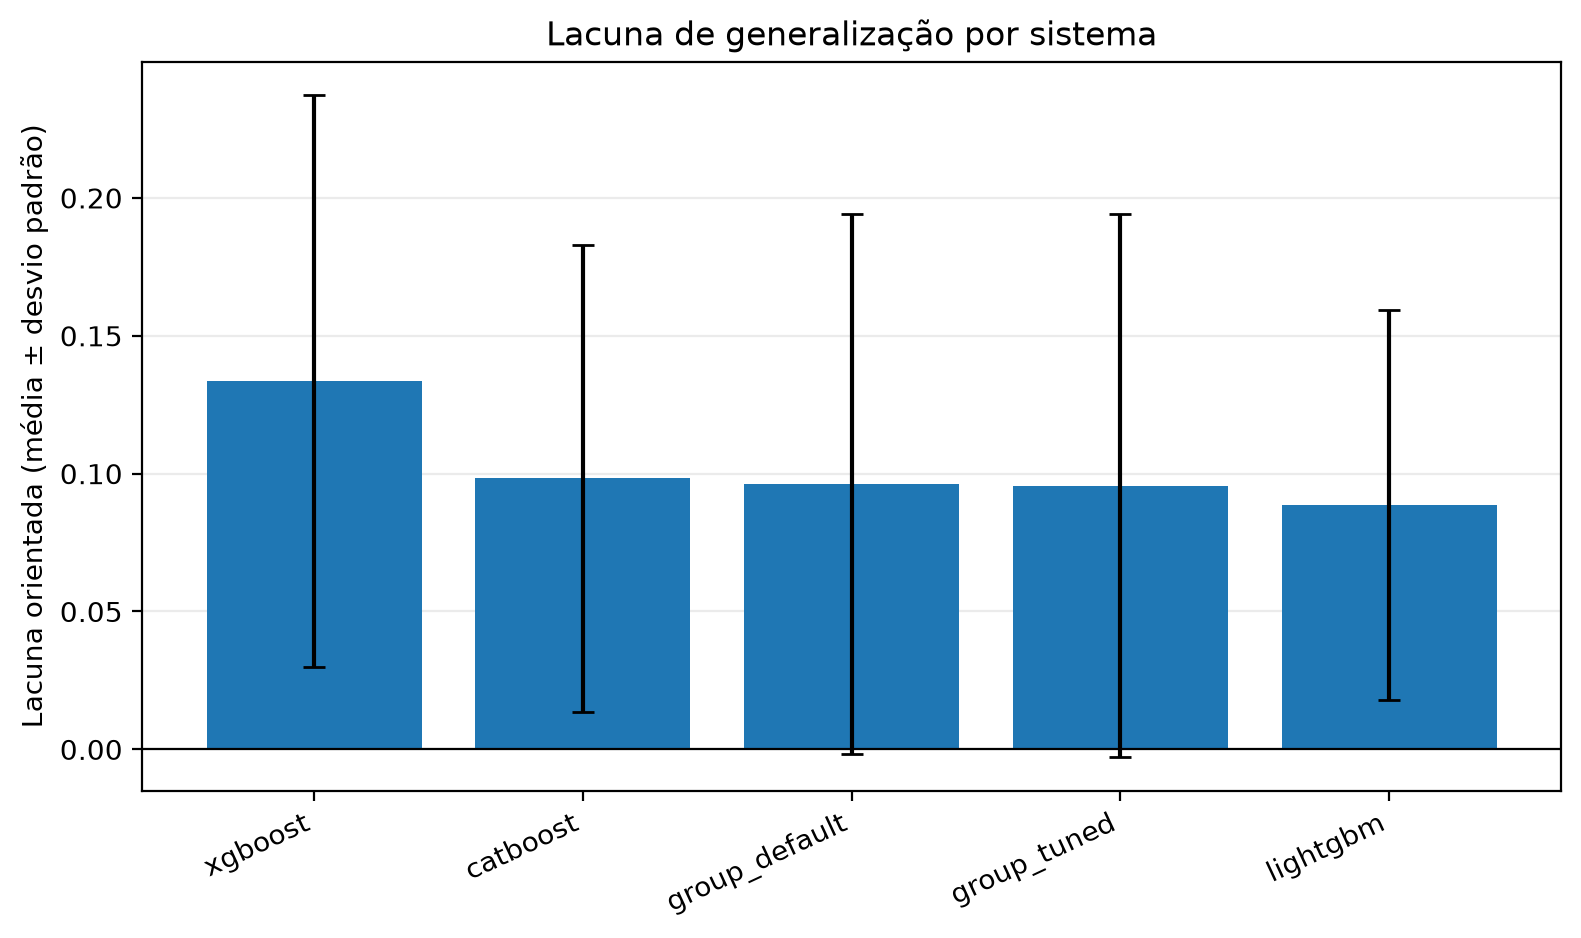
\includegraphics[width=0.78\textwidth]{../../../results/figures/lacuna_auc_ovo.png}
    \caption{Comparação entre AUC OvO média de treino interno, validação interna e lacuna de generalização para os cinco sistemas avaliados ($270$ partições internas por sistema).}
    \label{fig:lacuna}
\end{figure}

\paragraph{2. Curvas de validação de complexidade e regra de 1 erro padrão.}
Para confrontar diretamente o controle de capacidade estrutural do modelo tema com um baseline GBDT, geraram-se curvas de validação cruzada interna (no treino do fold externo 0 das três bases de estudo) variando $\texttt{n\_estimators} \in \{1, 2, 4, 8, 16, 32\}$ no TabICL v2 (\texttt{SIMPLER\_IS\_LOWER = True}) e $\texttt{num\_leaves} \in \{2, 4, 8, 16, 32, 64, 128\}$ no LightGBM (\texttt{SIMPLER\_IS\_LOWER = True}). A Tabela~\ref{tab:complexidade} sintetiza os pontos escolhidos pela melhor média (\texttt{best}) e pela regra de 1 erro padrão (\texttt{1se}), e a Figura~\ref{fig:curvas_complexidade} exibe os seis gráficos resultantes.

\begin{table}[htbp]
    \centering
    \caption{Seleção de complexidade pela melhor média (\texttt{best}) e pela regra de 1 erro padrão (\texttt{1se}) nas curvas de validação interna (AUC OvO, treino do fold externo 0).}
    \label{tab:complexidade}
    \small
    \resizebox{\textwidth}{!}{%
    \begin{tabular}{@{}llrrl@{}}
        \toprule
        \textbf{Regime (Dataset)} & \textbf{Sistema (Hiperparâmetro)} & \textbf{Melhor média} & \textbf{Regra de 1 EP} & \textbf{No \texttt{search\_space}?} \\
        \midrule
        Pequeno (\texttt{363621}) & TabICL v2 (\texttt{n\_estimators}) & $16$ ($0{,}7552$) & $1$ ($0{,}7525$) & Fixado em $8$ a priori \\
        Médio (\texttt{363704}) & TabICL v2 (\texttt{n\_estimators}) & $16$ ($0{,}8849$) & $4$ ($0{,}8837$) & Fixado em $8$ a priori \\
        Grande (\texttt{363628}) & TabICL v2 (\texttt{n\_estimators}) & $32$ ($0{,}9915$) & $1$ ($0{,}9906$) & Fixado em $8$ a priori \\
        \midrule
        Pequeno (\texttt{363621}) & LightGBM (\texttt{num\_leaves}) & $4$ & $4$ & Baseline fixo (\texttt{pytabkit}) \\
        Médio (\texttt{363704}) & LightGBM (\texttt{num\_leaves}) & $8$ & $4$ & Baseline fixo (\texttt{pytabkit}) \\
        Grande (\texttt{363628}) & LightGBM (\texttt{num\_leaves}) & $16$ & $8$ & Baseline fixo (\texttt{pytabkit}) \\
        \bottomrule
    \end{tabular}
    }%
\end{table}

\begin{figure}[htbp]
    \centering
    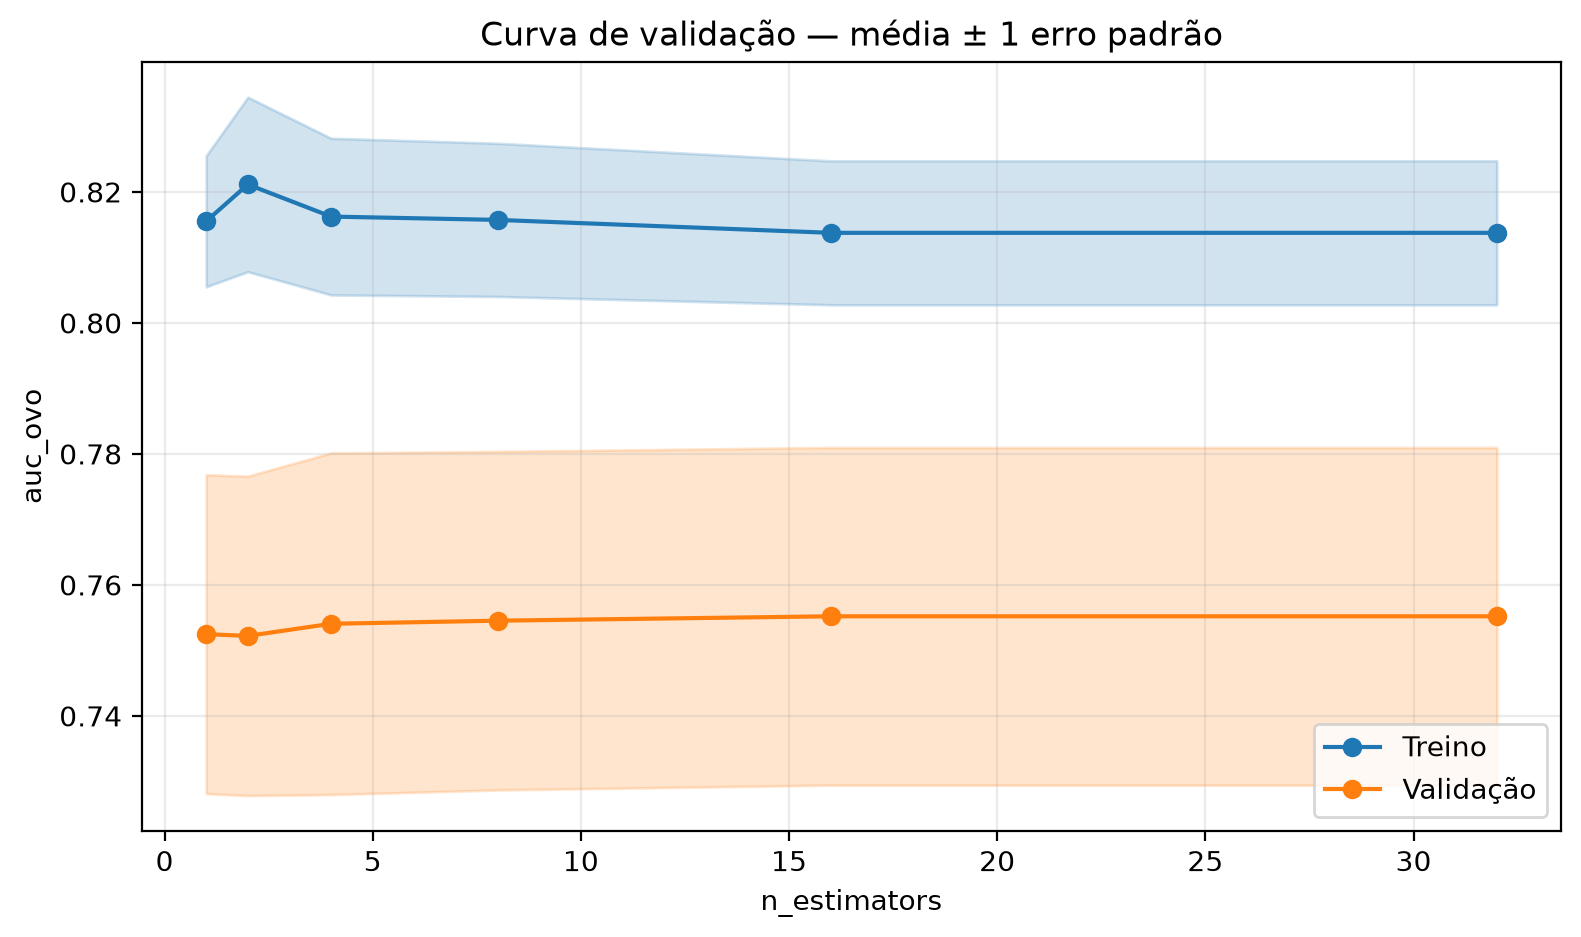
\includegraphics[width=0.32\textwidth]{../../../results/figures/curva_grupo_363621.png}\hfill
    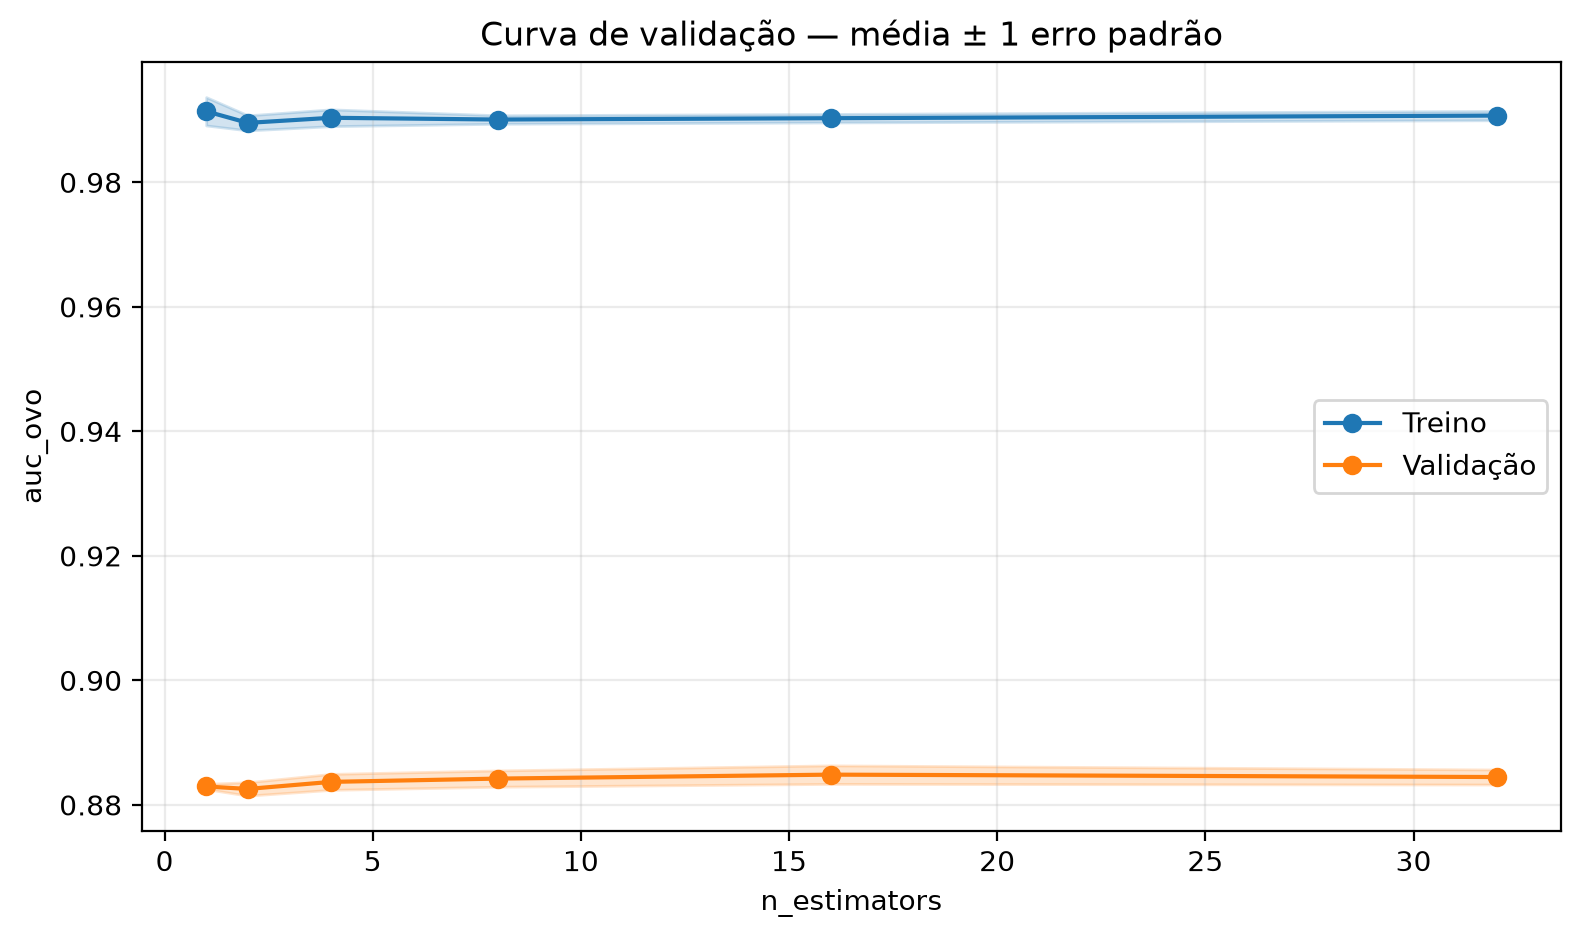
\includegraphics[width=0.32\textwidth]{../../../results/figures/curva_grupo_363704.png}\hfill
    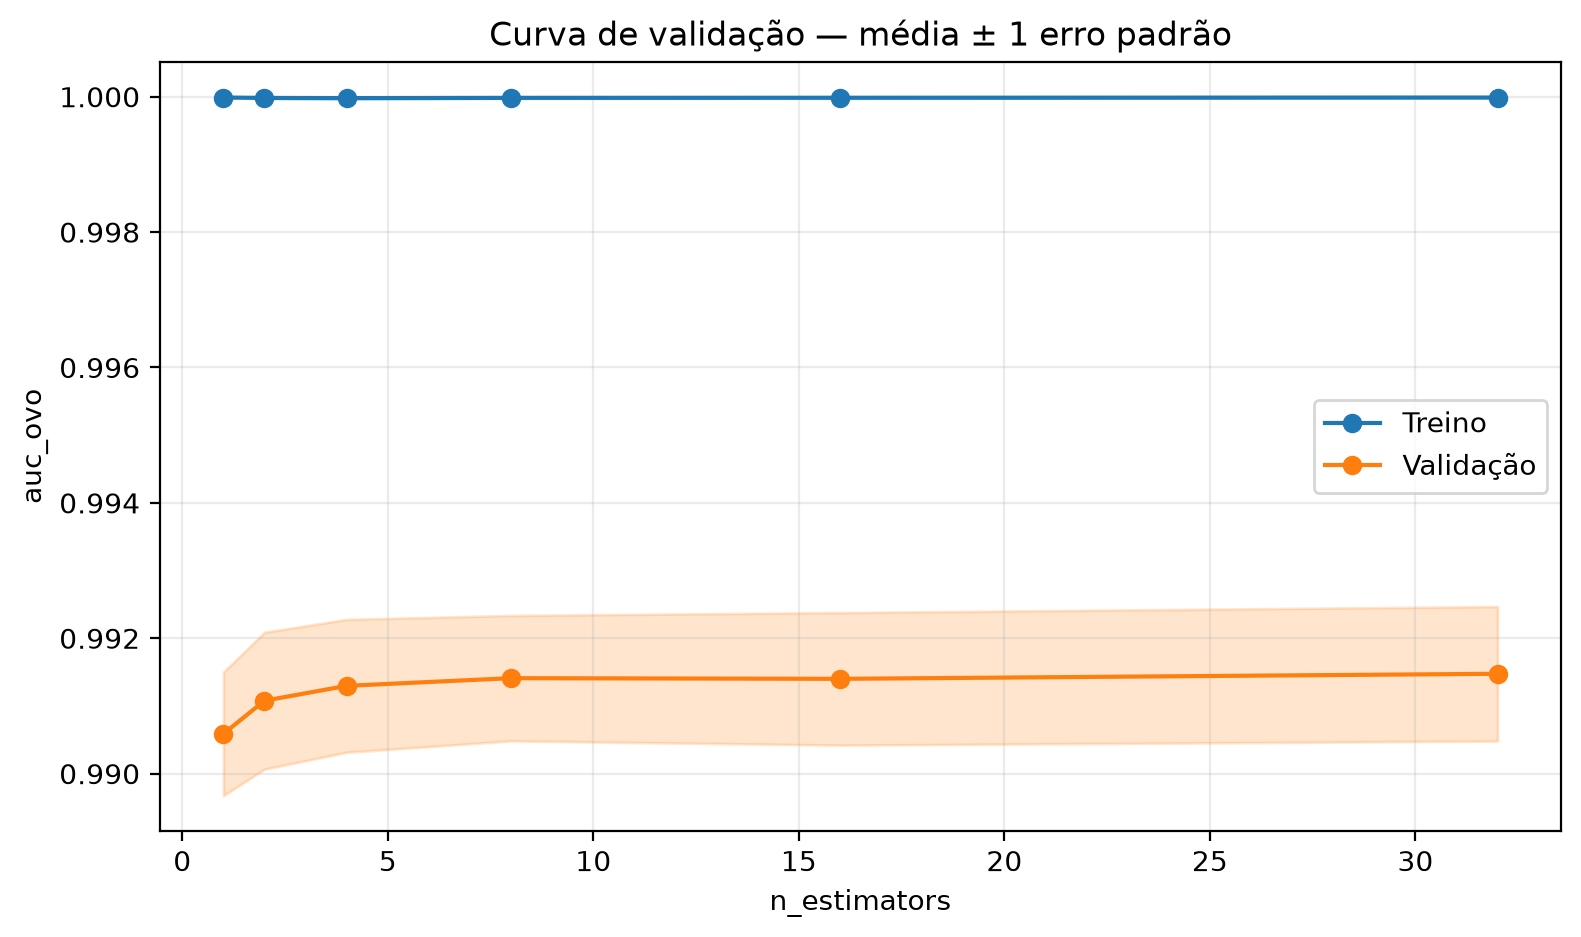
\includegraphics[width=0.32\textwidth]{../../../results/figures/curva_grupo_363628.png}\\[0.6em]
    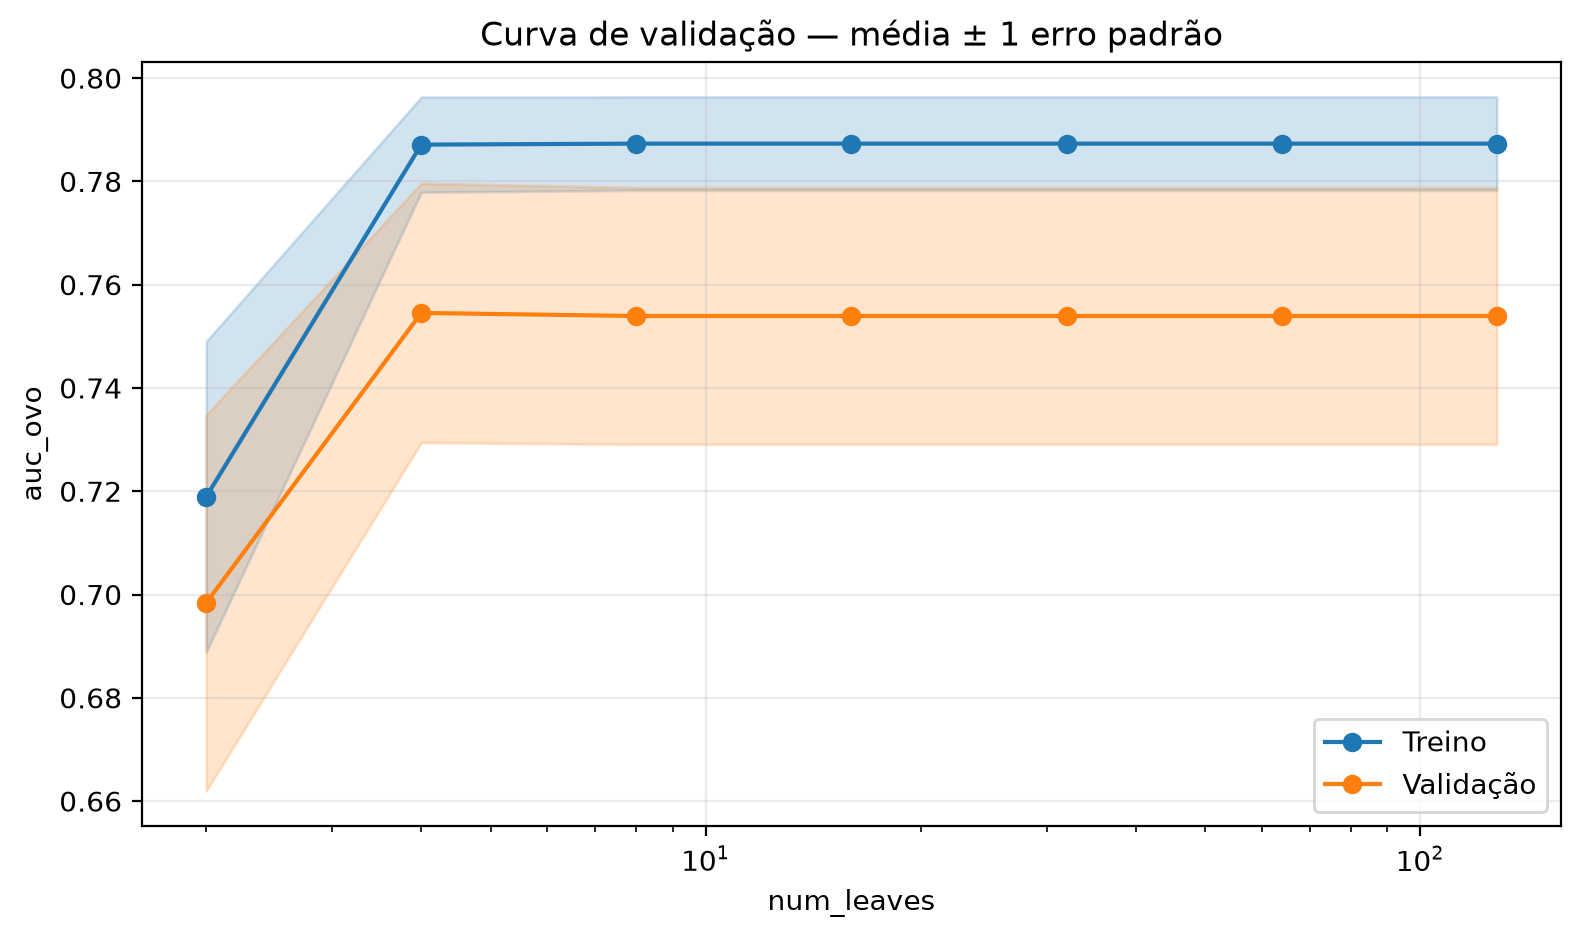
\includegraphics[width=0.32\textwidth]{../../../results/figures/curva_lgbm_363621.png}\hfill
    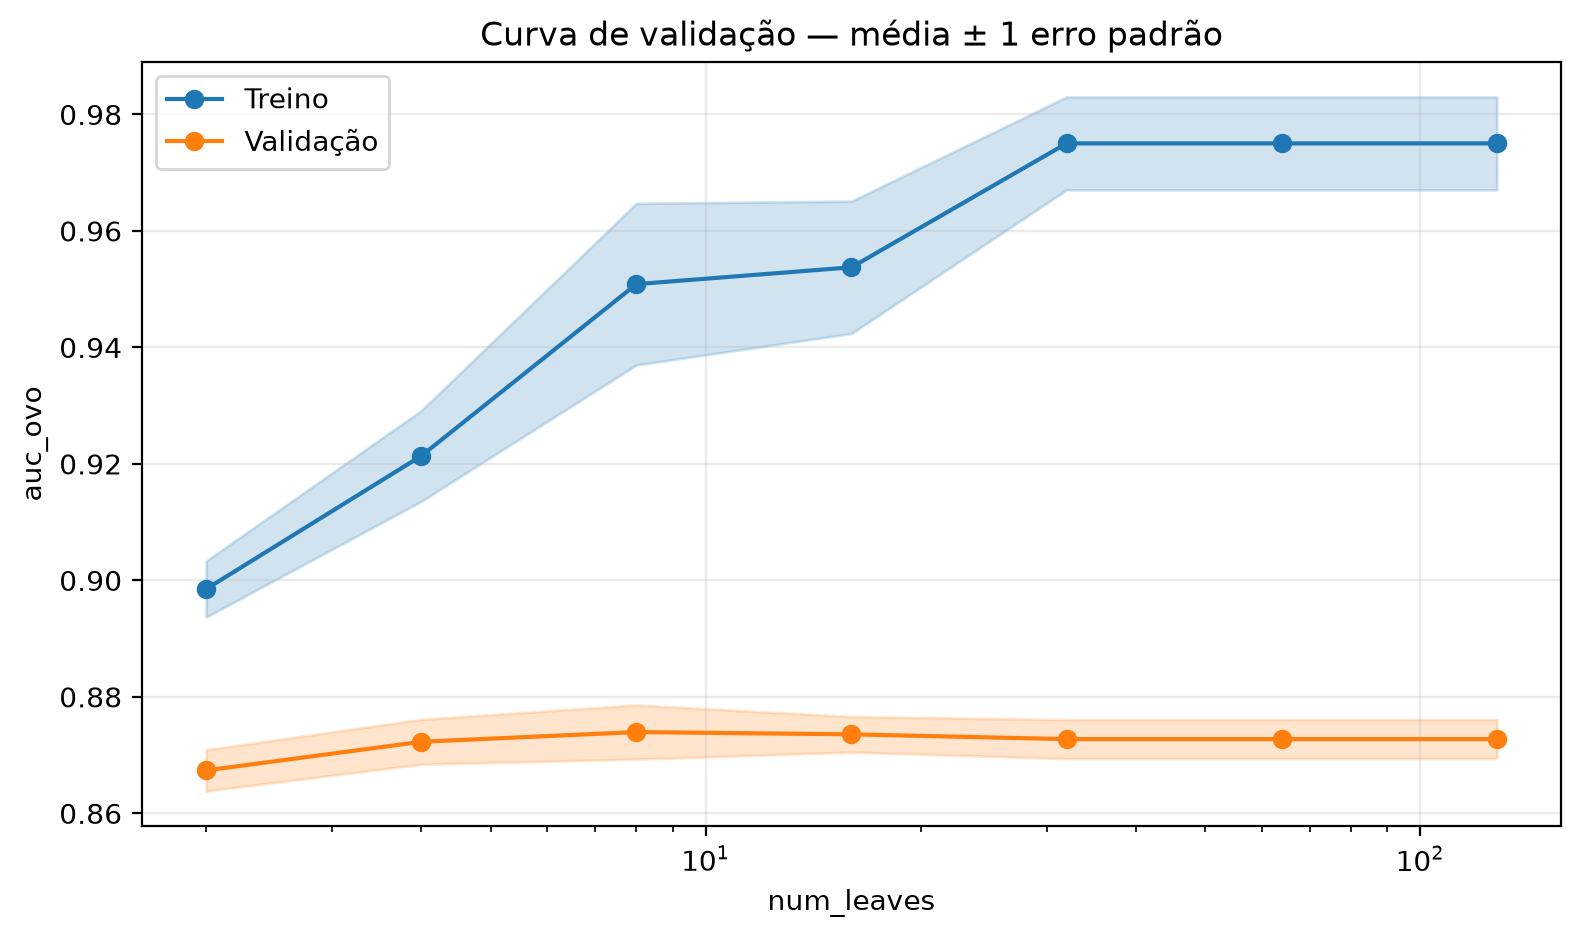
\includegraphics[width=0.32\textwidth]{../../../results/figures/curva_lgbm_363704.png}\hfill
    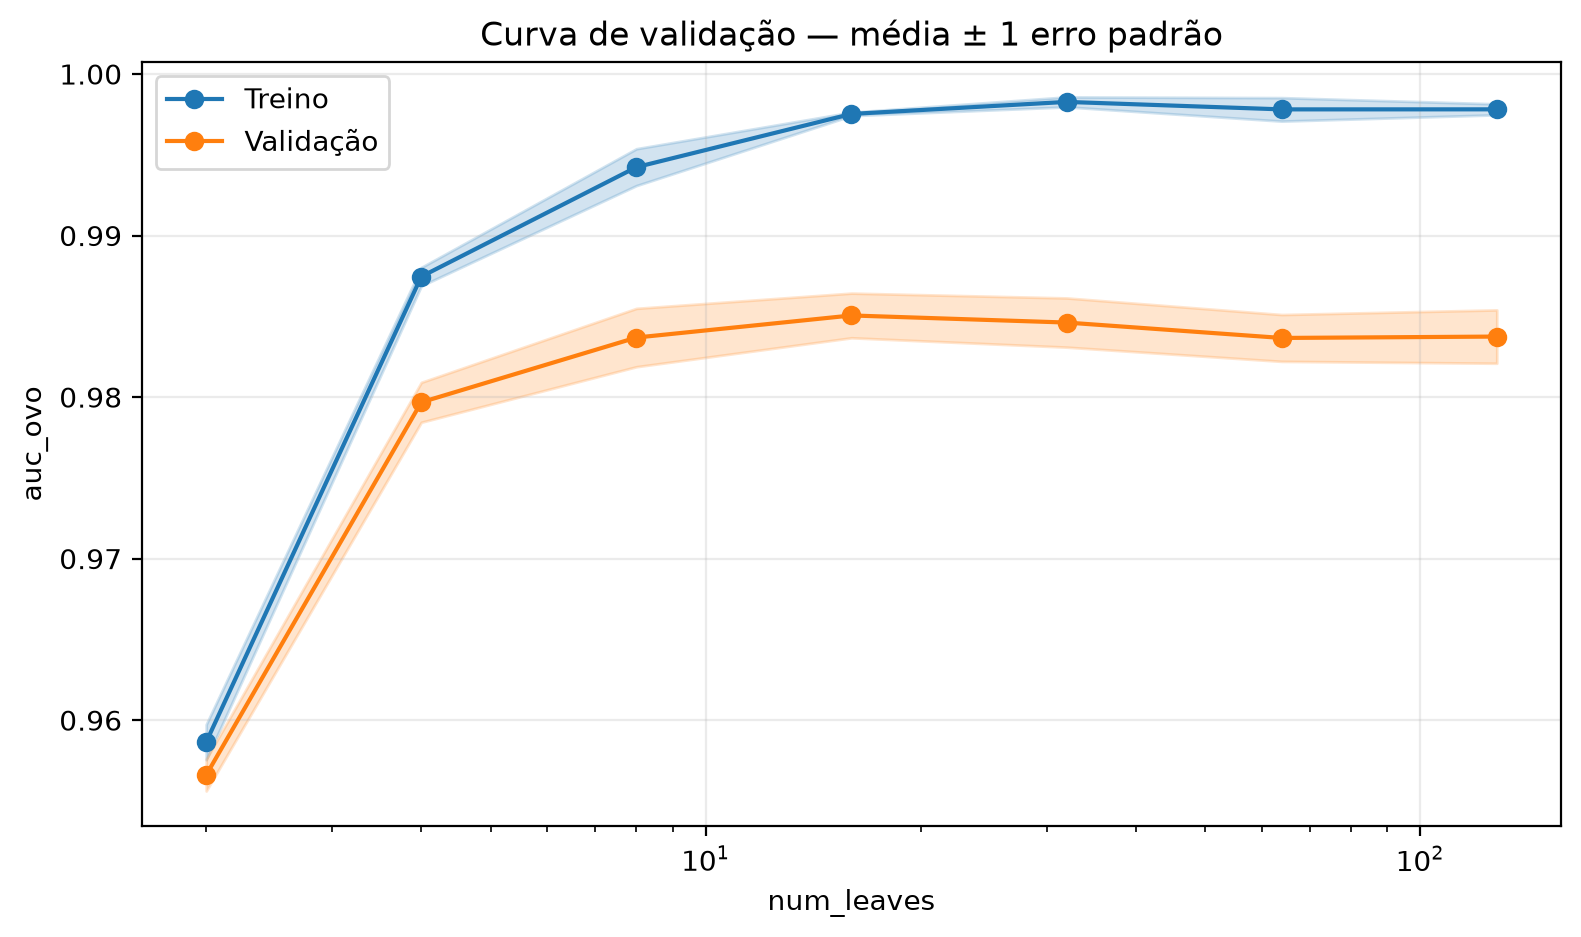
\includegraphics[width=0.32\textwidth]{../../../results/figures/curva_lgbm_363628.png}
    \caption{Curvas de validação interna (AUC OvO $\pm 1\text{ EP}$) nos datasets pequeno (\texttt{363621}, esquerda), médio (\texttt{363704}, centro) e grande (\texttt{363628}, direita). Linha superior: TabICL v2 variando \texttt{n\_estimators}. Linha inferior: LightGBM variando \texttt{num\_leaves} (escala logarítmica).}
    \label{fig:curvas_complexidade}
\end{figure}

\paragraph{3. Matrizes de confusão e erros por classe na validação interna.}
Somando as predições fora da amostra das 3 partições internas do fold externo 0 (\texttt{results/preds\_val/}), calcularam-se as matrizes de confusão normalizadas por linha e os recalls por classe para os cinco sistemas (Figura~\ref{fig:confusao_val}).

\begin{figure}[htbp]
    \centering
    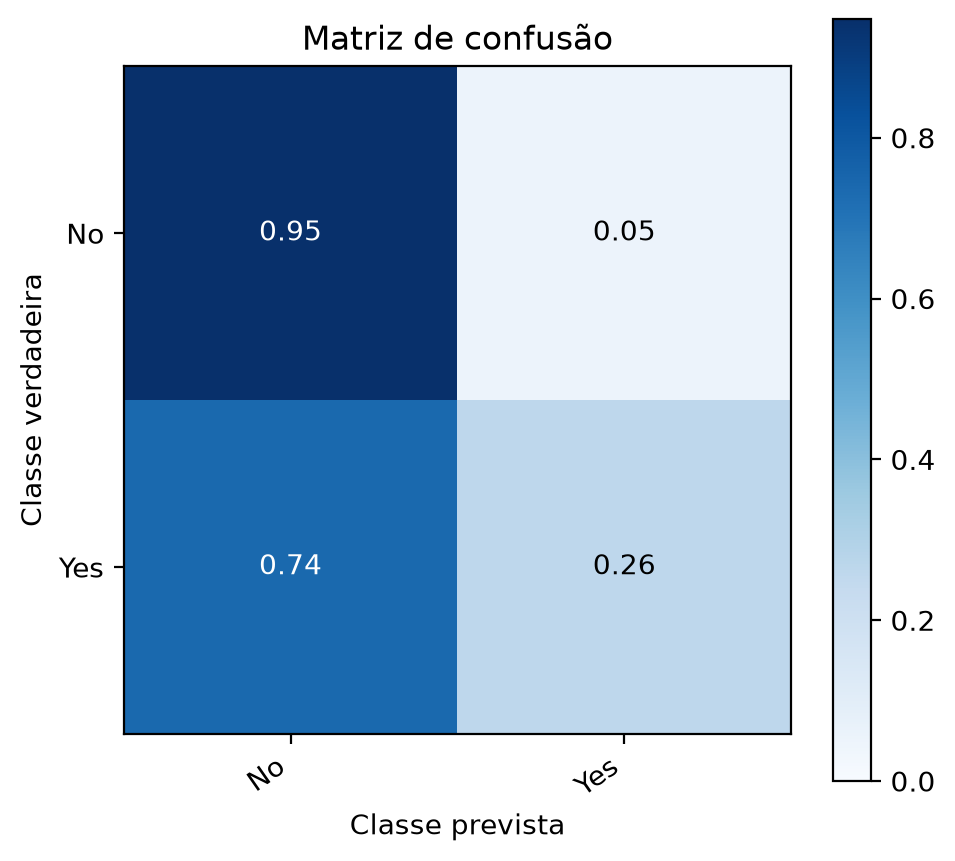
\includegraphics[width=0.31\textwidth]{../../../results/figures/confusao_363621_group_tuned.png}\hfill
    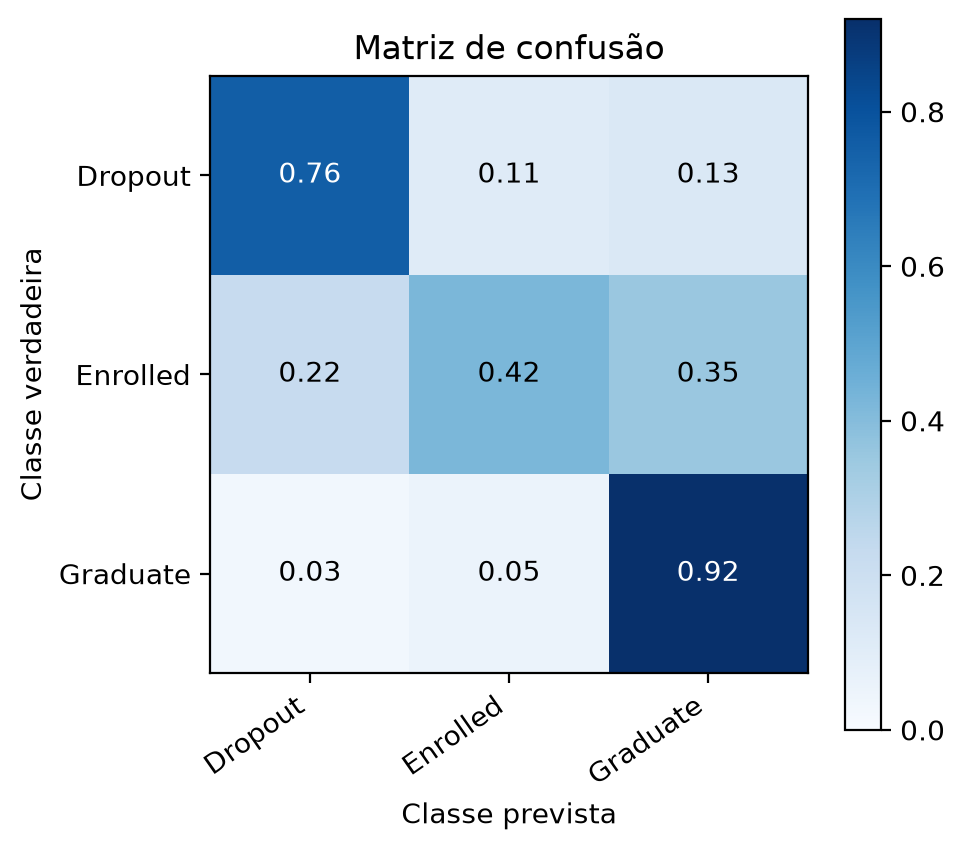
\includegraphics[width=0.31\textwidth]{../../../results/figures/confusao_363704_group_tuned.png}\hfill
    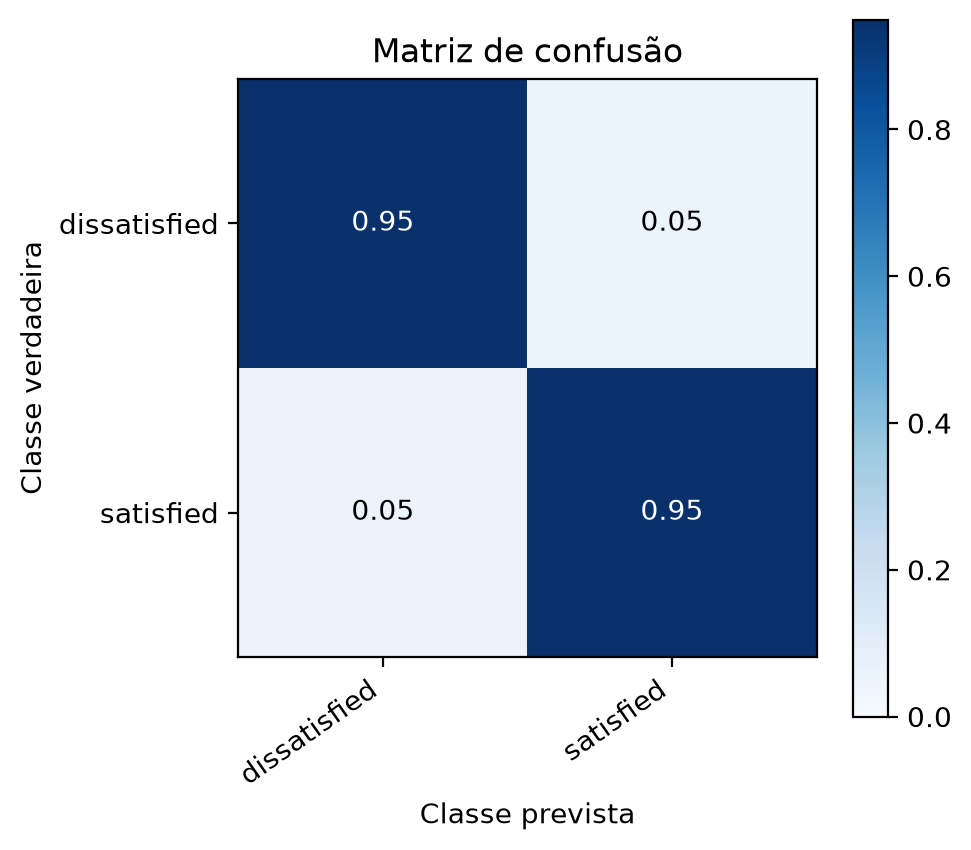
\includegraphics[width=0.31\textwidth]{../../../results/figures/confusao_363628_group_tuned.png}\\[0.5em]
    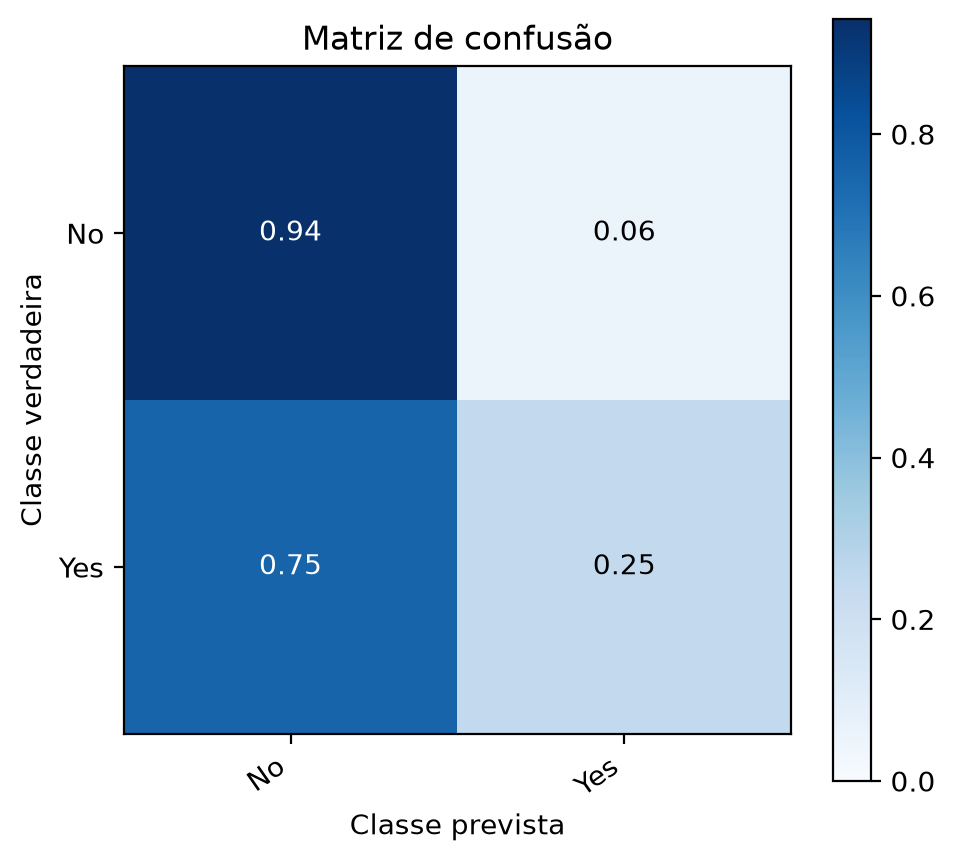
\includegraphics[width=0.31\textwidth]{../../../results/figures/confusao_363621_lightgbm.png}\hfill
    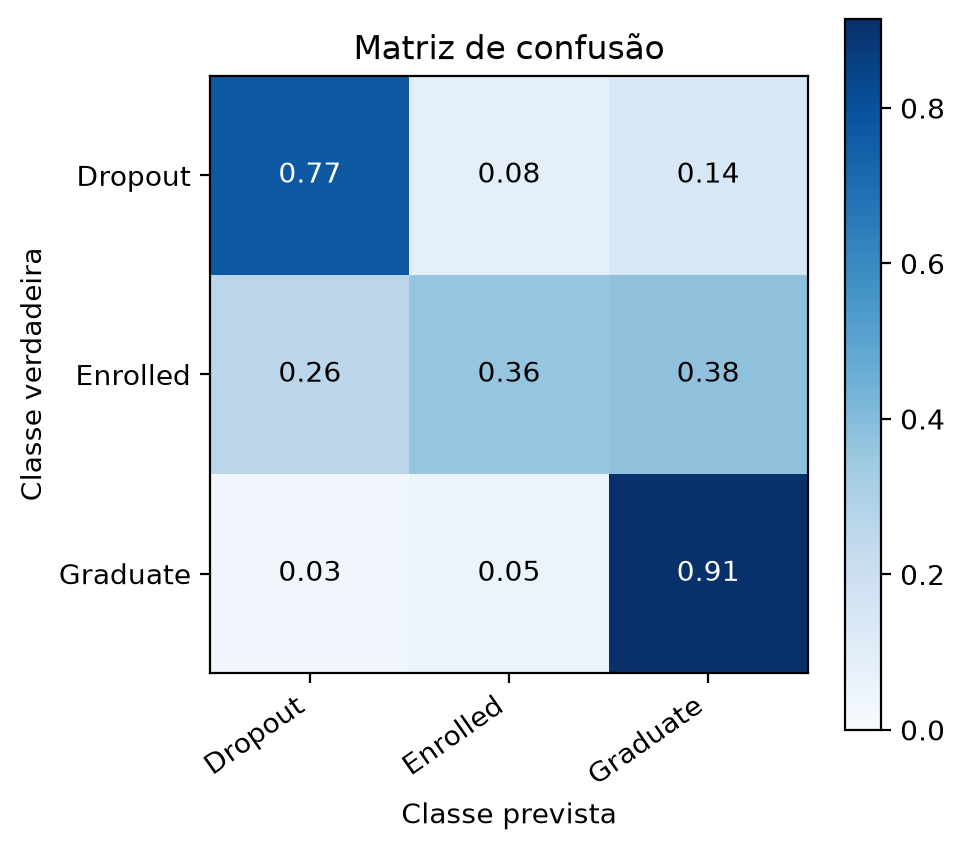
\includegraphics[width=0.31\textwidth]{../../../results/figures/confusao_363704_lightgbm.png}\hfill
    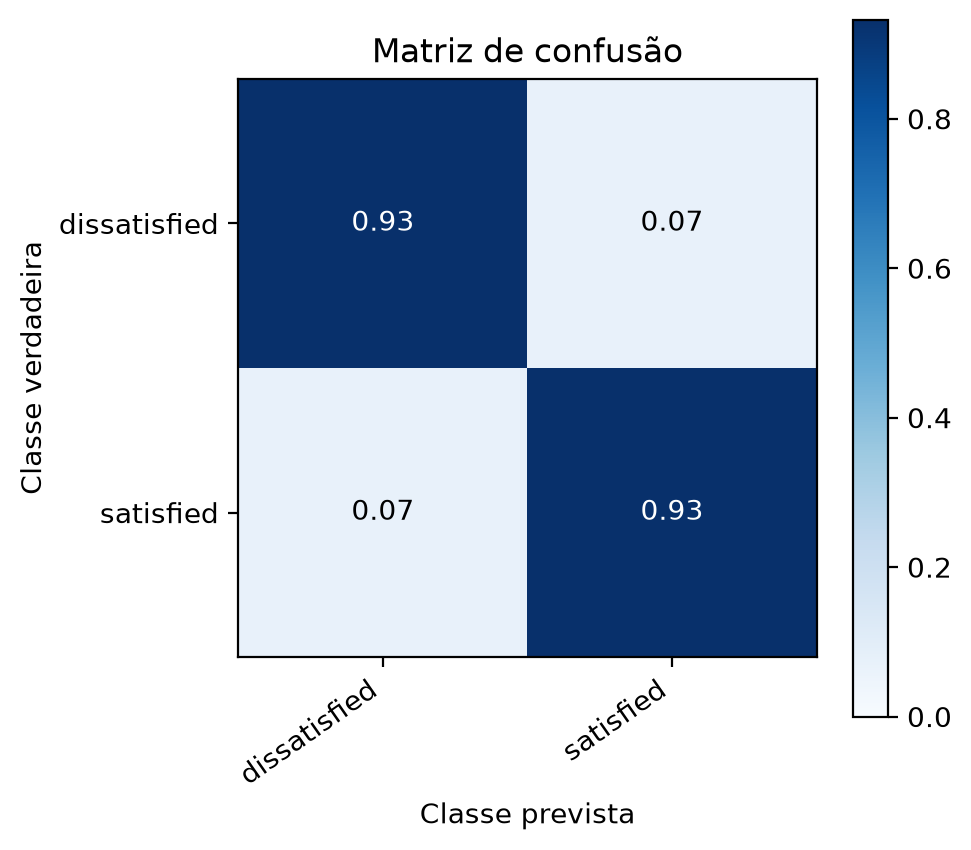
\includegraphics[width=0.31\textwidth]{../../../results/figures/confusao_363628_lightgbm.png}
    \caption{Matrizes de confusão normalizadas por linha (diagonal principal equivale ao recall por classe) somadas nas 3 partições de validação interna do fold externo 0 para \texttt{group\_tuned} (linha superior) e \texttt{lightgbm} (linha inferior) nos datasets \texttt{363621} (pequeno, binário), \texttt{363704} (médio, 3 classes) e \texttt{363628} (grande, binário).}
    \label{fig:confusao_val}
\end{figure}

\paragraph{Respostas integradas às 7 perguntas do notebook 05:}
\begin{enumerate}[leftmargin=2em]
    \item \textbf{Sistemas com maior lacuna, efeito do regime pequeno e compromisso viés-variância (Pergunta 1):} globalmente, a maior lacuna treino-validação ocorre no \texttt{xgboost} ($0{,}1335 \pm 0{,}1038$), seguido por \texttt{catboost} ($0{,}0983$), \texttt{group\_default} ($0{,}0963$), \texttt{group\_tuned} ($0{,}0955$) e \texttt{lightgbm} ($0{,}0886$). Nos baselines XGBoost e CatBoost, a lacuna é acentuadamente maior nos datasets pequenos ($0{,}1585$ e $0{,}1313$) e cai monotonicamente nos médios ($0{,}1348$ e $0{,}0996$) e grandes ($0{,}1071$ e $0{,}0640$). Segundo Hastie, Tibshirani e Friedman \cite{hastie2009elements} (Seções 2.9 e 7.3), ensembles de árvores profundas possuem baixo viés e alta flexibilidade; quando $n$ é pequeno, particionam finamente o espaço de atributos memorizando ruído amostral ($\text{AUC}_{\mathrm{treino}} \approx 0{,}96$), o que infla a variância e derruba a generalização ($\text{AUC}_{\mathrm{val}} = 0{,}8056$ no XGBoost pequeno). Já no LightGBM (\emph{Tuned Defaults}), restrições de suporte mínimo por folha limitam a profundidade efetiva quando $n$ é pequeno ($\text{AUC}_{\mathrm{treino}} = 0{,}9010$, lacuna de $0{,}0715$). No TabICL v2, cumpre destacar uma cautela teórica fundamental: a pontuação elevada de treino ($\approx 0{,}951$) não decorre de ajuste paramétrico de pesos, mas do fato de que, ao predizer uma subamostra do próprio conjunto de treino na inferência em contexto, cada exemplo consultado já está presente no contexto do $\mathrm{TF}_{\mathrm{icl}}$ acompanhado de seu rótulo verdadeiro no \emph{Target-Aware Embedding};
    \item \textbf{Ponto de estagnação nas curvas de complexidade por regime (Pergunta 2):} no LightGBM (\texttt{num\_leaves}), o ponto ótimo de validação desloca-se positivamente com o tamanho amostral: em \texttt{363621} (pequeno, $n_{\mathrm{tr}} = 498$), treino e validação atingem um platô conjunto já em $\texttt{num\_leaves} = 4$; em \texttt{363704} (médio, $n_{\mathrm{tr}} = 2.949$), a validação atinge o máximo em $\texttt{num\_leaves} = 8$ e recua a partir de $16$ enquanto o treino segue rumo a $1{,}0$; em \texttt{363628} (grande, $n_{\mathrm{tr}} = 10.000$), o volume de dados sustenta partições mais finas e a validação cresce até $\texttt{num\_leaves} = 16$. No TabICL v2 (\texttt{n\_estimators}), aumentar $E$ reduz a variância por agregação de visões sem aumentar a capacidade individual do Transformer: a curva de treino permanece plana ($\approx 0{,}815$, $0{,}990$ e $0{,}99998$), enquanto a validação apresenta retornos decrescentes suaves, estabilizando na prática a partir de $E = 8$ ou $16$;
    \item \textbf{Escolha pela regra de 1 EP e relação com \texttt{search\_space} (Pergunta 3):} em 5 das 6 curvas (Tabela~\ref{tab:complexidade}), a regra de 1 erro padrão \cite{breiman1984classification} selecionou um modelo estritamente mais parcimonioso que o ponto de melhor média ($\texttt{num\_leaves} = 4$ e $8$ em vez de $8$ e $16$ no LightGBM médio/grande; $E = 1$, $4$ e $1$ em vez de $16$, $16$ e $32$ no TabICL v2). A regra de 1 EP é uma heurística de parcimônia que escolhe o modelo mais simples dentro de um erro padrão $\text{EP}(v^\star) = s(v^\star)/\sqrt{K}$ da melhor média, reduzindo variância nos GBDTs e tempo de inferência no TabICL v2. Como declarado a priori, \texttt{n\_estimators} permaneceu fixo em $8$ no \texttt{search\_space}, valor situado dentro da faixa de 1 EP da melhor média nos três regimes;
    \item \textbf{Otimismo da validação de \texttt{group\_tuned} e papel da CV aninhada (Pergunta 4):} em \texttt{validation.csv}, as linhas de \texttt{group\_tuned} possuem $\texttt{optimistic} = \texttt{True}$ porque os hiperparâmetros $\hat{\theta}$ foram selecionados maximizando a AUC OvO exatamente nas mesmas 3 partições internas em que o modelo é avaliado ($\mathbb{E}[\max_\theta \hat{M}_{\mathrm{val}}(\theta)] > \max_\theta \mathbb{E}[\hat{M}_{\mathrm{val}}(\theta)]$, caracterizando otimismo de seleção \cite{cawley2010overfitting,varma2006bias}). A validação cruzada aninhada corrige esse viés ao confinar toda a busca do Optuna dentro do treino de cada fold externo $f$ e avaliar o estimador retreinado com $\hat{\theta}_f$ uma única vez no teste externo selado do fold $f$;
    \item \textbf{Vedação ao uso do teste externo nos estudos diagnósticos (Pergunta 5):} na divisão de 3 folds externos do TabArena, o treino de um fold externo contém o teste dos outros dois. Se curvas de complexidade ou escolhas de \texttt{search\_space} consultassem \texttt{results/test.csv}, ocorreria vazamento direto de informação (\emph{human-in-the-loop overfitting}), invalidando todas as garantias frequentistas dos testes de hipótese finais;
    \item \textbf{Concentração de erros por classe, G-Mean vs. AUC OvO e comparação com GBDTs (Pergunta 6):} nas predições de validação interna do fold 0, os erros concentram-se nas classes minoritárias ou intermediárias: em \texttt{363621} (suporte: 380 \texttt{No} vs. 118 \texttt{Yes}), o recall de \texttt{No} varia de $0{,}8921$ a $0{,}9474$, enquanto o recall da classe minoritária \texttt{Yes} cai para $0{,}1780$ (\texttt{xgboost}), $0{,}2458$ (\texttt{lightgbm}), $0{,}2627$ (\texttt{group\_tuned}), $0{,}2712$ (\texttt{group\_default}) e $0{,}3305$ (\texttt{catboost}), resultando em G-Mean entre $0{,}4106$ (XGBoost) e $0{,}5430$ (CatBoost). No problema de 3 classes \texttt{363704} (1.472 \texttt{Graduate}, 947 \texttt{Dropout}, 530 \texttt{Enrolled}), a classe intermediária \texttt{Enrolled} concentra a maior taxa de confusão, mas o TabICL v2 alcança o maior recall nessa classe difícil ($0{,}4264$ em \texttt{group\_default} e $0{,}4226$ em \texttt{group\_tuned}, contra $0{,}3491$ no XGBoost e $0{,}3642$ no LightGBM), elevando o G-Mean do TabICL para $0{,}6663$ contra $0{,}6219$ do XGBoost. Já em \texttt{363628} (balanceado), todas as classes superam $0{,}93$ de recall, com liderança do TabICL ($\text{G-Mean} = 0{,}9477$). Isso evidencia que uma AUC OvO moderada/alta (que mede ordenação global em todos os limiares) pode coexistir com baixo recall na decisão \texttt{argmax} sob desbalanceamento severo;
    \item \textbf{Uso exclusivo de \texttt{preds\_val/} e imutabilidade do \texttt{protocolo.lock} (Pergunta 7):} somar as matrizes de confusão das 3 partições internas de \texttt{results/preds\_val/} fornece predições fora da amostra para todo o conjunto de desenvolvimento sem tocar no teste externo; contudo, exatamente por compartilhar amostras entre folds externos distintos, essas observações diagnósticas não podem jamais motivar alterações retrospectivas do espaço de busca ou do \texttt{protocolo.lock}.
\end{enumerate}

\subsection{Implementação}
\label{sec:implementacao}

Todos os módulos exigidos pelo protocolo foram implementados de forma limpa e determinística: \texttt{src/models/group\_model.py} (classe \texttt{AdaptiveTabICLClassifier}, fábrica \texttt{build\_group\_model} e função \texttt{search\_space}), \texttt{src/models/wrappers.py} (codificação ordinal de categorias em \texttt{ImputedClassifier}), \texttt{src/pipeline/tune.py} (tratamento de \texttt{NonFiniteProbabilityError} durante trials do Optuna), \texttt{src/pipeline/demsar.py} (testes de Friedman, Iman-Davenport, Holm, Bonferroni-Dunn, Nemenyi, Wilcoxon signed-ranks e diagramas CD), \texttt{src/pipeline/bootstrap.py} (intervalos de confiança por percentil via reamostragem com reposição), \texttt{src/pipeline/overfitting.py} (cálculo de lacuna treino-validação, curvas de complexidade e seleção por \texttt{best} e \texttt{1se}), \texttt{src/pipeline/class\_errors.py} (matrizes de confusão e recalls por classe), \texttt{src/pipeline/regime.py} (agregação e ranqueamento por regime) e \texttt{src/reports/plots\_overfitting.py}.

A suíte automatizada de testes unitários e de contrato foi verificada integralmente com a variável de ambiente \texttt{AM\_STRICT=1 pytest}, aprovando todos os testes de seleção de datasets (\texttt{test\_selection.py}), integridade anti-vazamento (\texttt{test\_integrity.py}), contrato do modelo do grupo (\texttt{test\_group\_model.py}), pipeline de avaliação (\texttt{test\_pipeline.py}), estatística de Demšar (\texttt{test\_demsar.py}), sobreajuste (\texttt{test\_overfitting.py}) e bootstrap (\texttt{test\_bootstrap.py}).

\subsection{Avaliação final}
\label{sec:val_vs_test}

Após o congelamento do protocolo (\texttt{python -m src.pipeline.freeze}) e o commit de \texttt{results/protocolo.lock} (\texttt{9718c9649b}), a avaliação final do teste externo selado foi realizada por \texttt{src.pipeline.final\_test}. As primeiras execuções ocorreram no Google Colab com GPU NVIDIA Tesla T4; as duas combinações finais que continuavam com erro de memória foram recuperadas no Kaggle, mediante \texttt{--resume}, usando o mesmo protocolo e o histórico Git transferido. Foram concluídas todas as $450$ combinações ($30\text{ datasets} \times 3\text{ folds externos} \times 5\text{ sistemas}$), com $\texttt{status} = \texttt{ok}$, sem exclusões pela regra de completude ($N = 30$ datasets completos).

O registro \texttt{results/test\_log.csv} documenta \textbf{uma avaliação inicial e quatro retomadas} ($490$ eventos no total). Na primeira execução, o backend interativo do Matplotlib configurado no Colab gerou falhas na inicialização de baselines; a configuração do ambiente para \texttt{MPLBACKEND=Agg} permitiu retomar as combinações pendentes. Uma interrupção posterior de sessão exigiu nova retomada. As duas combinações restantes, \texttt{363628|1|group\_tuned} e \texttt{363628|2|group\_tuned}, falharam por insuficiência de memória para uma alocação estimada em aproximadamente $12.684\text{ MB}$, sem descarregamento em disco habilitado nesse caso. O dataset possui $129.880$ instâncias no total; os conjuntos de teste dos folds 1 e 2 possuem \textbf{$43.293$ instâncias cada}, e não $86.587$. As duas avaliações foram concluídas no ambiente Kaggle, sem alteração do código ou dos hiperparâmetros congelados. A evidência disponível não permite atribuir a falha exclusivamente à fragmentação ou ao acúmulo de memória CUDA. Nenhuma combinação anteriormente concluída com sucesso foi reavaliada nas retomadas, conforme \texttt{check\_protocol}.

A Tabela~\ref{tab:val_vs_test} confronta o desempenho médio entre datasets na validação interna (média dos 9 folds internos por dataset em \texttt{validation.csv}) e na avaliação final (média dos 3 folds externos de teste em \texttt{test.csv}) para a métrica primária (AUC OvO) e para a métrica secundária (entropia cruzada).

\begin{table}[htbp]
    \centering
    \caption{Comparação entre validação interna (\texttt{results/validation.csv}, $270$ partições internas por sistema) e teste externo selado (\texttt{results/test.csv}, $90$ folds externos por sistema) nas métricas primária (AUC OvO) e secundária (entropia cruzada).}
    \label{tab:val_vs_test}
    \small
    \resizebox{\textwidth}{!}{%
    \begin{tabular}{@{}lrrrr@{}}
        \toprule
        \textbf{Sistema} & \textbf{AUC OvO (val.)} & \textbf{AUC OvO (teste)} & \textbf{Entropia cruzada (val.)} & \textbf{Entropia cruzada (teste)} \\
        \midrule
        \texttt{group\_default} & $0{,}8542 \pm 0{,}1149$ & $\mathbf{0{,}8607} \pm 0{,}1170$ & $\mathbf{0{,}3147} \pm 0{,}1645$ & $\mathbf{0{,}3005} \pm 0{,}1633$ \\
        \texttt{group\_tuned} & $\mathbf{0{,}8556} \pm 0{,}1147$ & $0{,}8606 \pm 0{,}1166$ & $0{,}3285 \pm 0{,}1676$ & $0{,}3150 \pm 0{,}1673$ \\
        \texttt{lightgbm} & $0{,}8304 \pm 0{,}1192$ & $0{,}8407 \pm 0{,}1190$ & $0{,}3610 \pm 0{,}1651$ & $0{,}3447 \pm 0{,}1613$ \\
        \texttt{catboost} & $0{,}8328 \pm 0{,}1157$ & $0{,}8405 \pm 0{,}1159$ & $0{,}4493 \pm 0{,}1774$ & $0{,}4551 \pm 0{,}2569$ \\
        \texttt{xgboost} & $0{,}8190 \pm 0{,}1277$ & $0{,}8281 \pm 0{,}1259$ & $0{,}4932 \pm 0{,}2433$ & $0{,}4277 \pm 0{,}2120$ \\
        \bottomrule
    \end{tabular}
    }%
\end{table}

Observam-se dois comportamentos metodologicamente reveladores na Tabela~\ref{tab:val_vs_test}: (i) todos os sistemas sem otimismo de seleção apresentaram AUC média superior no teste externo em relação à validação interna (por exemplo, \texttt{group\_default} sobe de $0{,}8542$ para $0{,}8607$ e \texttt{lightgbm} de $0{,}8304$ para $0{,}8407$), o que é compatível com o uso de maior volume de treinamento no ajuste final (até $10.000$ amostras), embora não permita atribuir causalmente toda a diferença observada a esse fator; e (ii) a vantagem aparente de $+0{,}0014$ que \texttt{group\_tuned} exibia sobre \texttt{group\_default} na validação interna ($0{,}8556$ vs. $0{,}8542$, inflada pelo otimismo de seleção) desaparece completamente no teste externo selado ($0{,}8606$ vs. $0{,}8607$).

\subsection{Resultados gerais}
\label{sec:resultados_gerais}

A Tabela~\ref{tab:resumo_geral} apresenta o resumo geral no conjunto de teste externo (\texttt{summary\_by\_model} do notebook \texttt{04\_analise\_estatistica.ipynb}), reportando a média e o desvio-padrão entre os $N = 30$ datasets (após agregação dos 3 folds externos de cada dataset) para as quatro métricas de qualidade preditiva e para os tempos de busca, treino, inferência e total. A Figura~\ref{fig:boxplot_auc} exibe a distribuição da métrica primária AUC OvO nos 30 datasets para os quatro sistemas principais da análise de Demšar.

\begin{table}[htbp]
    \centering
    \caption{Resumo geral no conjunto de teste externo ($N = 30$ datasets; média $\pm$ desvio-padrão das médias por dataset sobre os 3 folds externos).}
    \label{tab:resumo_geral}
    \small
    \resizebox{\textwidth}{!}{%
    \begin{tabular}{@{}lrrrrrrr@{}}
        \toprule
        \textbf{Sistema} & \textbf{AUC OvO} & \textbf{Acurácia} & \textbf{G-Mean} & \textbf{Entropia cruz.} & \textbf{Busca (s)} & \textbf{Treino (s)} & \textbf{Pred. (s)} \\
        \midrule
        \texttt{group\_default} & $\mathbf{0{,}8607} \pm 0{,}1170$ & $0{,}8703 \pm 0{,}0878$ & $\mathbf{0{,}6548} \pm 0{,}2915$ & $\mathbf{0{,}3005} \pm 0{,}1633$ & $0{,}00$ & $3{,}86$ & $18{,}38$ \\
        \texttt{group\_tuned} & $0{,}8606 \pm 0{,}1166$ & $\mathbf{0{,}8704} \pm 0{,}0877$ & $0{,}6541 \pm 0{,}2923$ & $0{,}3150 \pm 0{,}1673$ & $196{,}49$ & $3{,}58$ & $18{,}71$ \\
        \texttt{lightgbm} & $0{,}8407 \pm 0{,}1190$ & $0{,}8570 \pm 0{,}0905$ & $0{,}6187 \pm 0{,}2834$ & $0{,}3447 \pm 0{,}1613$ & $0{,}00$ & $2{,}76$ & $0{,}56$ \\
        \texttt{catboost} & $0{,}8405 \pm 0{,}1159$ & $0{,}8588 \pm 0{,}0866$ & $0{,}6370 \pm 0{,}2668$ & $0{,}4551 \pm 0{,}2569$ & $0{,}00$ & $4{,}54$ & $0{,}19$ \\
        \texttt{xgboost} & $0{,}8281 \pm 0{,}1259$ & $0{,}8548 \pm 0{,}0885$ & $0{,}6166 \pm 0{,}2718$ & $0{,}4277 \pm 0{,}2120$ & $0{,}00$ & $2{,}75$ & $0{,}21$ \\
        \bottomrule
    \end{tabular}
    }%
\end{table}

\begin{figure}[htbp]
    \centering
    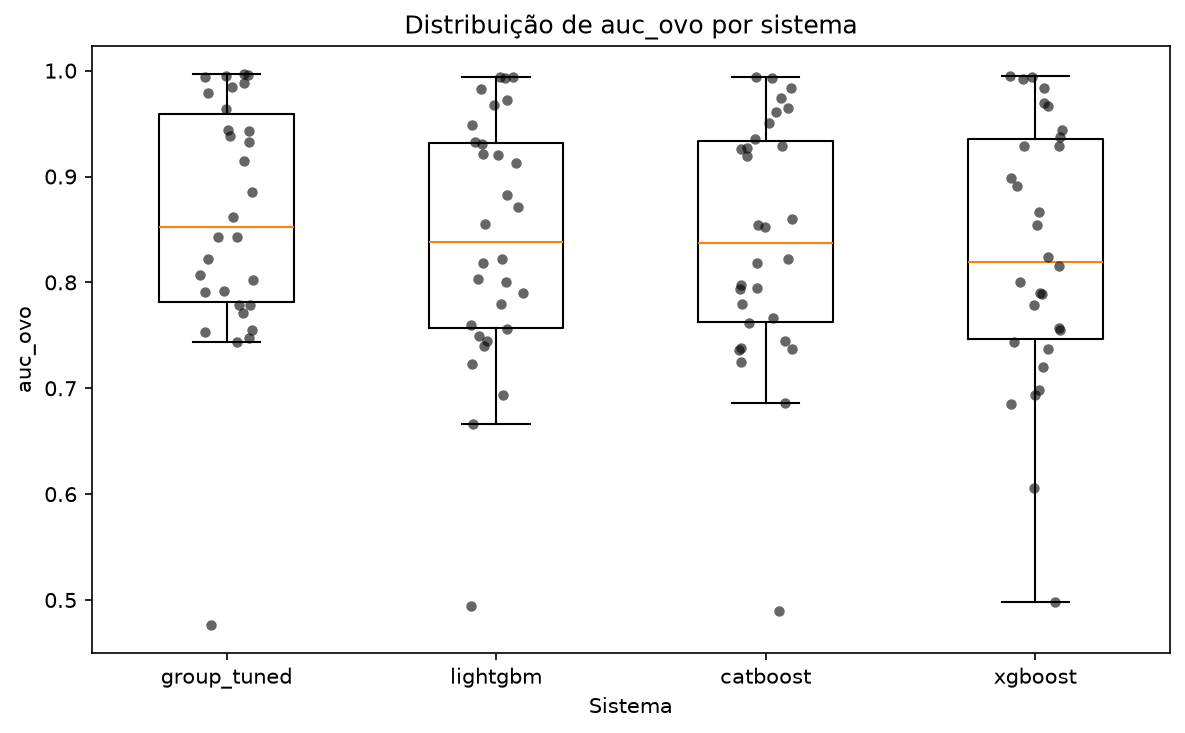
\includegraphics[width=0.75\textwidth]{../../../results/figures/boxplot_auc_ovo.png}
    \caption{Distribuição da AUC OvO média por dataset ($N = 30$) no conjunto de teste externo para os quatro sistemas comparados na análise principal.}
    \label{fig:boxplot_auc}
\end{figure}

As duas variantes do TabICL v2 lideram simultaneamente nas quatro métricas avaliadas: superam o melhor baseline em $+2{,}00$ pontos percentuais de AUC OvO média ($0{,}8607$ vs. $0{,}8407$ do LightGBM), em $+1{,}16\text{ p.p.}$ de acurácia ($0{,}8704$ vs. $0{,}8588$ do CatBoost), em $+1{,}78\text{ p.p.}$ de G-Mean ($0{,}6548$ vs. $0{,}6370$ do CatBoost) e reduzem a entropia cruzada média em $12{,}8\%$ em relação ao LightGBM ($0{,}3005$ vs. $0{,}3447$).

\subsection{Análise estatística (Demšar, 2006)}
\label{sec:demsar}

Seguindo a metodologia de Demšar \cite{demsar2006statistical}, a unidade de observação independente é o \textbf{dataset} ($N = 30$), utilizando a média sobre os 3 folds externos de cada dataset. A comparação múltipla principal envolve $k = 4$ sistemas (\texttt{group\_tuned} como método controle e os três baselines \texttt{lightgbm}, \texttt{xgboost} e \texttt{catboost}) ao nível de significância $\alpha = 0{,}05$.

\paragraph{1. Teste global de Friedman e correção de Iman-Davenport (AUC OvO).}
Na métrica primária AUC OvO, os postos médios obtidos (menor posto equivale a maior AUC) foram:
\begin{equation}
    R_{\texttt{group\_tuned}} = 1{,}300, \qquad
    R_{\texttt{lightgbm}} = 2{,}633, \qquad
    R_{\texttt{catboost}} = 2{,}867, \qquad
    R_{\texttt{xgboost}} = 3{,}200.
\end{equation}
A estatística qui-quadrado de Friedman atingiu $\chi^2_F = 37{,}480$ ($p = 3{,}642 \times 10^{-8}$ com $k - 1 = 3$ graus de liberdade), e a estatística corrigida de Iman-Davenport resultou em:
\begin{equation}
    F_F = \frac{(N - 1)\chi^2_F}{N(k - 1) - \chi^2_F} = 20{,}695, \qquad \text{gl} = (3, 87), \qquad p = 3{,}284 \times 10^{-10}.
\end{equation}
Como $p = 3{,}284 \times 10^{-10} \ll 0{,}05$, rejeita-se com folga a hipótese nula de equivalência global de postos médios, habilitando os testes post-hoc.

\paragraph{2. Comparações post-hoc com controle (Holm e Bonferroni-Dunn) e todos contra todos (Nemenyi).}
Com $k = 4$ e $N = 30$, o erro padrão das diferenças de postos médios é $\mathrm{SE} = \sqrt{k(k+1)/(6N)} = \sqrt{20/180} = 1/3 \approx 0{,}3333$. As Tabelas~\ref{tab:holm_wilcoxon} e~\ref{tab:wilcoxon_baselines} apresentam, respectivamente, os resultados do procedimento sequencial de Holm e do teste pareado de Wilcoxon signed-ranks contra o controle \texttt{group\_tuned}, tanto para a métrica primária (AUC OvO) quanto para a métrica secundária (entropia cruzada). As Figuras~\ref{fig:cd_auc} e~\ref{fig:cd_ce} exibem os diagramas de diferença crítica (CD) de Bonferroni-Dunn ($\mathrm{CD}_{\mathrm{BD}} = 0{,}798$) e de Nemenyi ($\mathrm{CD}_{\mathrm{Nem}} = 0{,}856$).

\begin{table}[htbp]
    \centering
    \caption{Comparações post-hoc com \texttt{group\_tuned} como controle: procedimento de Holm aplicado aos postos de Friedman ($N=30$, $\alpha=0{,}05$).}
    \label{tab:holm_wilcoxon}
    \small
    \begin{tabular}{@{}llrrr@{}}
        \toprule
        \textbf{Métrica} & \textbf{Baseline} & $R_i-R_c$ & $z$ & $p_{\mathrm{Holm}}$ \\
        \midrule
        AUC OvO & \texttt{lightgbm} & $1{,}333$ & $4{,}000$ & $6{,}33\times10^{-5}$ \\
        AUC OvO & \texttt{catboost} & $1{,}567$ & $4{,}700$ & $5{,}20\times10^{-6}$ \\
        AUC OvO & \texttt{xgboost} & $1{,}900$ & $5{,}700$ & $3{,}59\times10^{-8}$ \\
        \midrule
        Entropia cruzada & \texttt{lightgbm} & $0{,}700$ & $2{,}100$ & $0{,}0357$ \\
        Entropia cruzada & \texttt{catboost} & $1{,}700$ & $5{,}100$ & $6{,}79\times10^{-7}$ \\
        Entropia cruzada & \texttt{xgboost} & $1{,}867$ & $5{,}600$ & $6{,}43\times10^{-8}$ \\
        \bottomrule
    \end{tabular}
\end{table}

\begin{table}[htbp]
    \centering
    \caption{Comparações pareadas com o controle (Wilcoxon signed-ranks e ajuste de Holm); vitórias, empates e derrotas do \texttt{group\_tuned} por dataset.}
    \label{tab:wilcoxon_baselines}
    \small
    \begin{tabular}{@{}llrrr@{}}
        \toprule
        \textbf{Métrica} & \textbf{Baseline} & \textbf{Vit./Emp./Der.} & $T$ & $p_{\mathrm{Holm}}$ \\
        \midrule
        AUC OvO & \texttt{lightgbm} & $27/0/3$ & $23{,}0$ & $2{,}38\times10^{-6}$ \\
        AUC OvO & \texttt{catboost} & $27/0/3$ & $19{,}0$ & $1{,}72\times10^{-6}$ \\
        AUC OvO & \texttt{xgboost} & $27/0/3$ & $22{,}0$ & $2{,}38\times10^{-6}$ \\
        \midrule
        Entropia cruzada & \texttt{lightgbm} & $22/0/8$ & $75{,}0$ & $7{,}30\times10^{-4}$ \\
        Entropia cruzada & \texttt{catboost} & $28/0/2$ & $17{,}0$ & $1{,}16\times10^{-6}$ \\
        Entropia cruzada & \texttt{xgboost} & $27/0/3$ & $24{,}0$ & $2{,}84\times10^{-6}$ \\
        \bottomrule
    \end{tabular}
    \par\vspace{0.4em}
    {\footnotesize Na entropia cruzada, a diferença \texttt{group\_tuned} versus \texttt{lightgbm} é significativa por Holm ($p=0{,}0357$), mas não supera as diferenças críticas de Bonferroni-Dunn ($0{,}798$) ou Nemenyi ($0{,}856$).}
\end{table}

\begin{figure}[htbp]
    \centering
    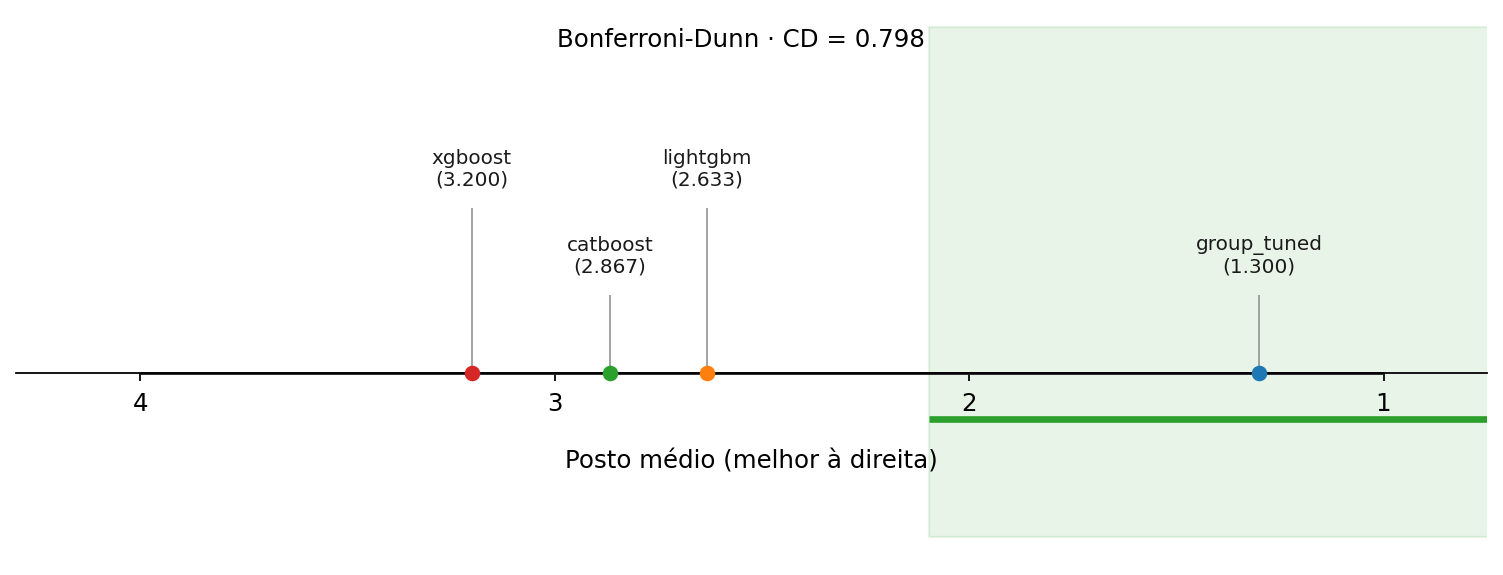
\includegraphics[width=0.86\textwidth]{../figuras/cd_bonferroni_dunn_auc_ovo.png}\par\vspace{0.5em}
    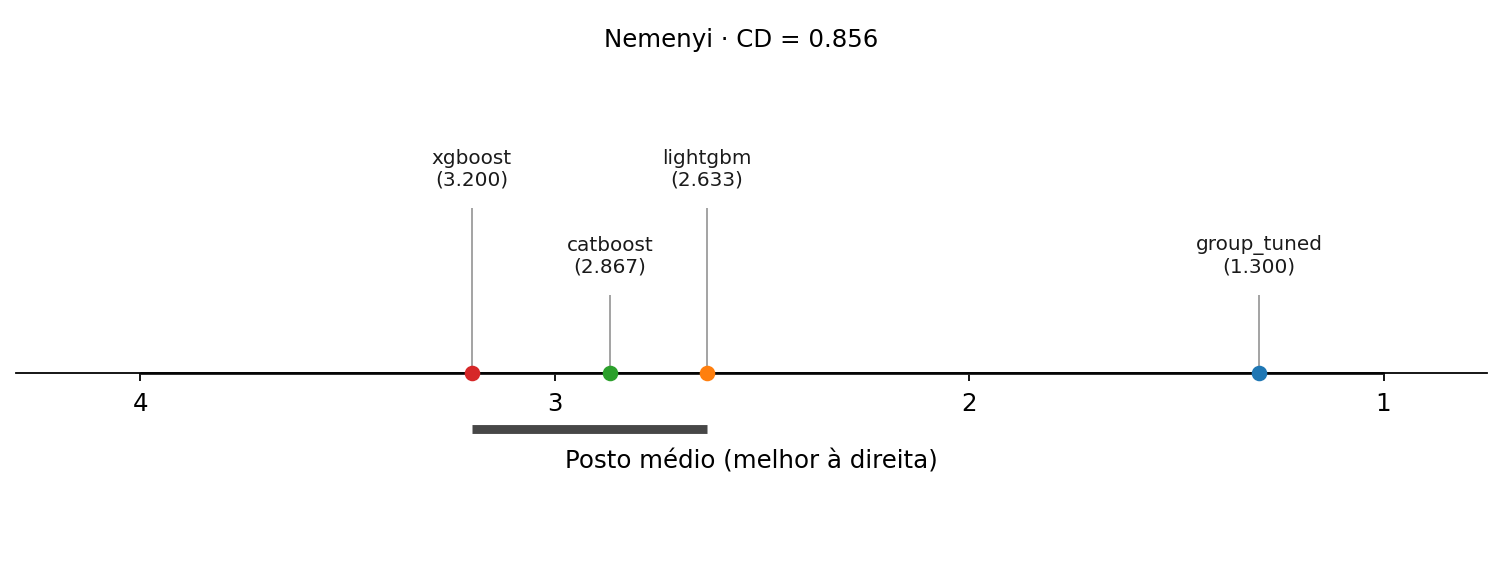
\includegraphics[width=0.86\textwidth]{../figuras/cd_nemenyi_auc_ovo.png}
    \caption{Diagramas de diferença crítica (CD) para a métrica primária \textbf{AUC OvO} ($N = 30$, $\alpha = 0{,}05$): Bonferroni-Dunn com \texttt{group\_tuned} como controle ($\mathrm{CD} = 0{,}798$, acima) e Nemenyi todos contra todos ($\mathrm{CD} = 0{,}856$, abaixo).}
    \label{fig:cd_auc}
\end{figure}

\begin{figure}[htbp]
    \centering
    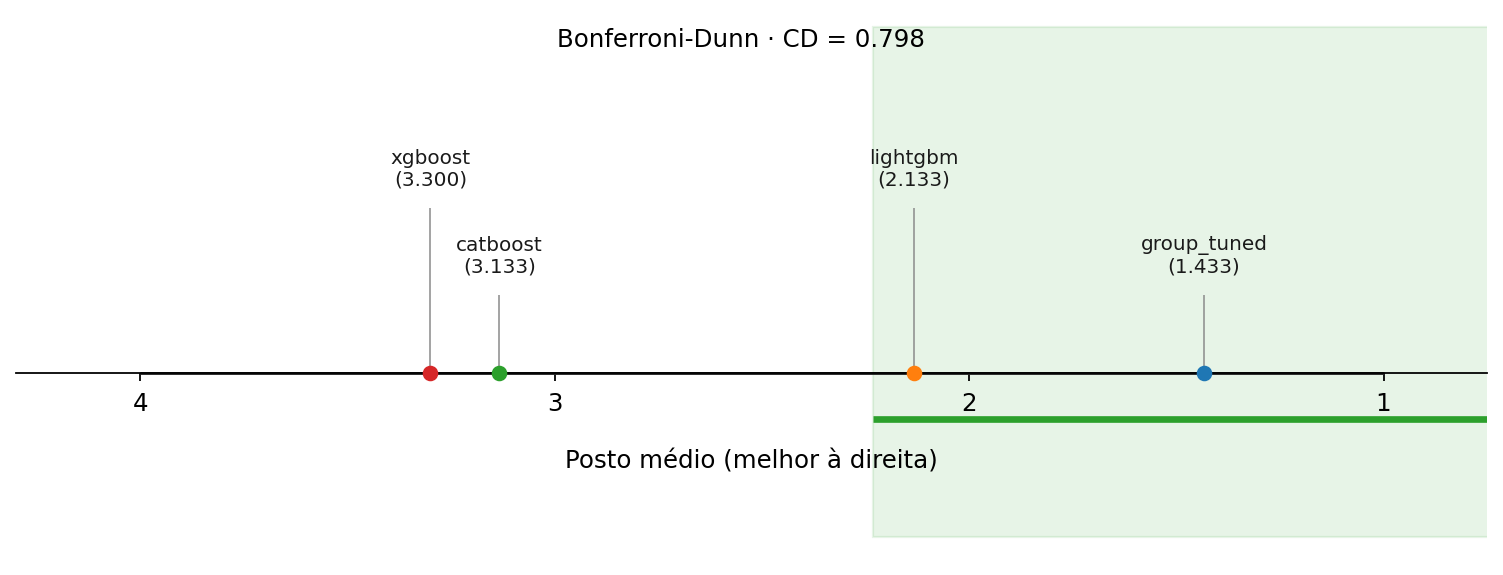
\includegraphics[width=0.86\textwidth]{../figuras/cd_bonferroni_dunn_cross_entropy.png}\par\vspace{0.5em}
    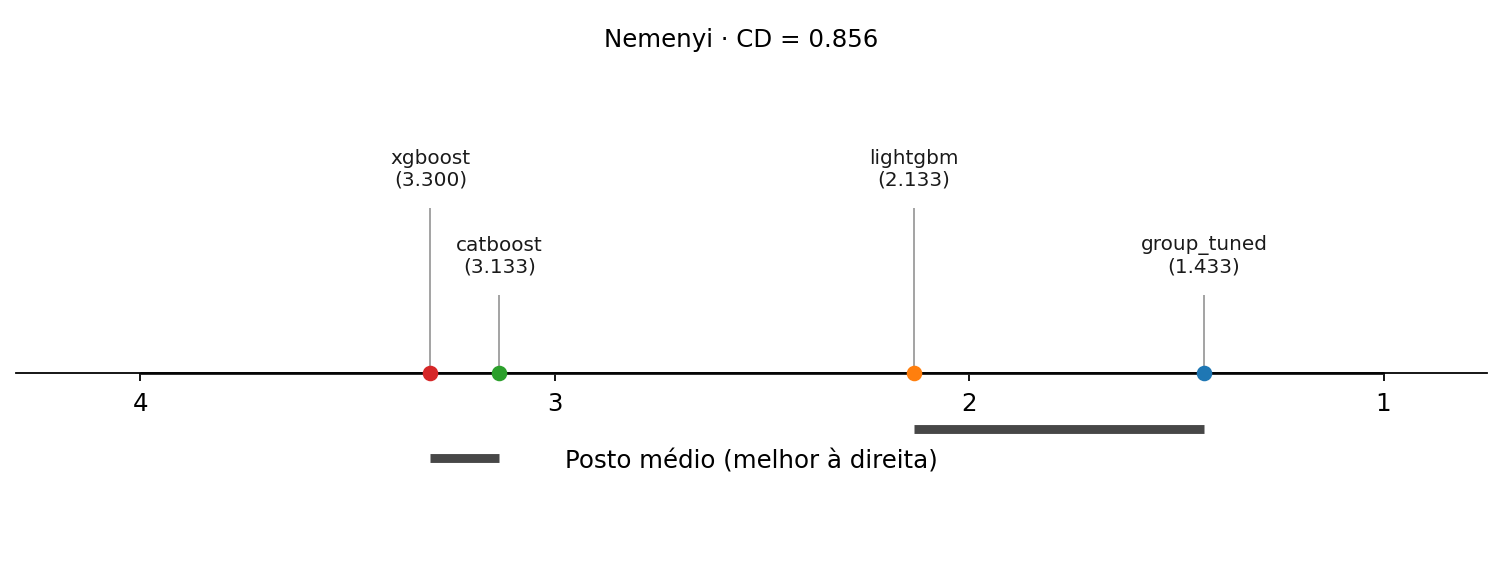
\includegraphics[width=0.86\textwidth]{../figuras/cd_nemenyi_cross_entropy.png}
    \caption{Diagramas de diferença crítica (CD) para a métrica secundária \textbf{entropia cruzada} ($N = 30$, $\alpha = 0{,}05$): Bonferroni-Dunn com \texttt{group\_tuned} como controle ($\mathrm{CD} = 0{,}798$, acima) e Nemenyi todos contra todos ($\mathrm{CD} = 0{,}856$, abaixo).}
    \label{fig:cd_ce}
\end{figure}

\paragraph{3. Comparação pareada entre \texttt{group\_default} e \texttt{group\_tuned} (Wilcoxon signed-ranks).}
Para avaliar descritivamente o efeito da busca de hiperparâmetros sobre o próprio modelo do grupo nos 30 datasets de teste:
\begin{itemize}[leftmargin=2em]
    \item Na \textbf{AUC OvO}, \texttt{group\_tuned} obteve 18 vitórias, 0 empates e 12 derrotas frente a \texttt{group\_default}, com somas de postos $R^+ = 281{,}0$ e $R^- = 184{,}0$, estatística $T = \min(R^+, R^-) = 184{,}0$ e $p = 0{,}3285$ (não significativo a $5\%$);
    \item Na \textbf{entropia cruzada} (menor é melhor), o quadro inverteu-se de forma contundente: \texttt{group\_tuned} obteve apenas 1 vitória (\texttt{credit-g}) e \textbf{29 derrotas} frente a \texttt{group\_default} ($R^+ = 1{,}0$, $R^- = 464{,}0$, $T = 1{,}0$, $p = 3{,}725 \times 10^{-9}$), indicando pior resultado na métrica probabilística de entropia cruzada para a variante otimizada, sem que tenha sido realizado teste específico de calibração.
\end{itemize}

\subsection{Incerteza no conjunto de teste}
\label{sec:bootstrap}

Para quantificar a incerteza amostral de cada estimativa de teste sem confundir variância interna de um fold com variância entre datasets, executou-se o bootstrap não paramétrico por percentil ($B = 1.000$ reamostragens com reposição das predições salvas em \texttt{results/preds/}, semente $42$) para todas as $450$ combinações de dataset, fold externo e sistema (\texttt{results/figures/bootstrap\_ci.csv}, detalhado no Apêndice~\ref{app:bootstrap}). A Tabela~\ref{tab:bootstrap_resumo} sintetiza a mediana, a média, o mínimo e o máximo da largura dos intervalos de confiança de $95\%$ ($\mathrm{width} = \mathrm{ci\_high} - \mathrm{ci\_low}$) na métrica primária AUC OvO.

\begin{table}[htbp]
    \centering
    \caption{Resumo da largura dos intervalos de confiança de 95\% por bootstrap ($B = 1.000$ reamostragens por dataset e fold externo; $90$ intervalos por sistema) para a métrica primária AUC OvO.}
    \label{tab:bootstrap_resumo}
    \small
    \begin{tabular}{@{}lrrrr@{}}
        \toprule
        \textbf{Sistema} & \textbf{Largura mediana} & \textbf{Largura média} & \textbf{Largura mínima} & \textbf{Largura máxima} \\
        \midrule
        \texttt{group\_tuned} & $\mathbf{0{,}0327}$ & $\mathbf{0{,}0477}$ & $0{,}0007$ & $0{,}1623$ \\
        \texttt{group\_default} & $0{,}0329$ & $0{,}0479$ & $0{,}0007$ & $0{,}1651$ \\
        \texttt{lightgbm} & $0{,}0388$ & $0{,}0531$ & $0{,}0008$ & $0{,}1639$ \\
        \texttt{catboost} & $0{,}0396$ & $0{,}0530$ & $0{,}0008$ & $0{,}1633$ \\
        \texttt{xgboost} & $0{,}0410$ & $0{,}0564$ & $0{,}0009$ & $0{,}1700$ \\
        \bottomrule
    \end{tabular}
\end{table}

Os resultados mostram que as duas configurações do TabICL v2 apresentam as menores larguras medianas de intervalo de confiança ($0{,}0327$ e $0{,}0329$, contra $0{,}0388$ a $0{,}0410$ nos baselines). Como a largura do IC de bootstrap é inversamente proporcional à raiz do tamanho do conjunto de teste e diminui conforme a AUC se aproxima de $1{,}0$, os intervalos mais largos ($\approx 0{,}14$ a $0{,}17$) concentram-se em bases pequenas ou severamente desbalanceadas (\texttt{blood-transfusion-service-center} com $n_{\mathrm{te}} = 250$ e \texttt{hiva\_agnostic} com razão de desbalanceamento $88{,}33$), enquanto nas bases grandes (\texttt{customer\_satisfaction\_in\_airline} e \texttt{SDSS17}) a largura é inferior a $0{,}002$.

\subsection{Análise por regime}
\label{sec:regimes}

A Tabela~\ref{tab:regimes} sintetiza o desempenho descritivo (média $\pm$ desvio-padrão de AUC OvO no teste externo) dos quatro sistemas principais ao longo dos quatro eixos de regime implementados em \texttt{src/pipeline/regime.py}, bem como o posto médio dentro de cada regime de tamanho.

\begin{table}[htbp]
    \centering
    \caption{Desempenho médio (AUC OvO no teste externo) e postos médios estratificados pelos quatro eixos de regime da suíte TabArena.}
    \label{tab:regimes}
    \small
    \resizebox{\textwidth}{!}{%
    \begin{tabular}{@{}llrrrrr@{}}
        \toprule
        \textbf{Eixo de regime} & \textbf{Estrato} & $N_{\text{cel}}$ & \texttt{group\_tuned} & \texttt{lightgbm} & \texttt{catboost} & \texttt{xgboost} \\
        \midrule
        Tamanho (AUC) & Pequeno ($n < 2.500$) & 10 & $\mathbf{0{,}8751} \pm 0{,}0950$ & $0{,}8423 \pm 0{,}1066$ & $0{,}8431 \pm 0{,}1008$ & $0{,}8158 \pm 0{,}1307$ \\
        Tamanho (AUC) & Médio ($2.500 \le n < 10.000$) & 10 & $\mathbf{0{,}8618} \pm 0{,}1582$ & $0{,}8442 \pm 0{,}1560$ & $0{,}8452 \pm 0{,}1544$ & $0{,}8351 \pm 0{,}1540$ \\
        Tamanho (AUC) & Grande ($n \ge 10.000$) & 10 & $\mathbf{0{,}8450} \pm 0{,}0963$ & $0{,}8355 \pm 0{,}0993$ & $0{,}8332 \pm 0{,}0961$ & $0{,}8334 \pm 0{,}1000$ \\
        \midrule
        Tamanho (Posto) & Pequeno / Médio / Grande & 10 & $\mathbf{1{,}00} / \mathbf{1{,}30} / \mathbf{1{,}60}$ & $2{,}90 / 2{,}80 / 2{,}20$ & $3{,}10 / 2{,}70 / 2{,}80$ & $3{,}00 / 3{,}20 / 3{,}40$ \\
        \midrule
        Tipo de problema & Binário ($C = 2$) & 24 & $\mathbf{0{,}8551} \pm 0{,}0893$ & $0{,}8325 \pm 0{,}0975$ & $0{,}8337 \pm 0{,}0934$ & $0{,}8161 \pm 0{,}1063$ \\
        Tipo de problema & Multiclasse ($C > 2$) & 6 & $\mathbf{0{,}8829} \pm 0{,}2036$ & $0{,}8735 \pm 0{,}1917$ & $0{,}8677 \pm 0{,}1916$ & $0{,}8762 \pm 0{,}1910$ \\
        \midrule
        Proporção categ. & Baixa ($< 25\%$) & 15 & $\mathbf{0{,}8759} \pm 0{,}0924$ & $0{,}8505 \pm 0{,}0990$ & $0{,}8524 \pm 0{,}0947$ & $0{,}8426 \pm 0{,}1036$ \\
        Proporção categ. & Alta ($\ge 25\%$) & 15 & $\mathbf{0{,}8454} \pm 0{,}1383$ & $0{,}8309 \pm 0{,}1390$ & $0{,}8286 \pm 0{,}1363$ & $0{,}8136 \pm 0{,}1471$ \\
        \midrule
        Valores ausentes & Sem ausentes (\texttt{no}) & 24 & $\mathbf{0{,}8549} \pm 0{,}1227$ & $0{,}8355 \pm 0{,}1251$ & $0{,}8370 \pm 0{,}1214$ & $0{,}8322 \pm 0{,}1249$ \\
        Valores ausentes & Com ausentes (\texttt{yes}) & 6 & $\mathbf{0{,}8837} \pm 0{,}0942$ & $0{,}8614 \pm 0{,}0975$ & $0{,}8544 \pm 0{,}0994$ & $0{,}8117 \pm 0{,}1407$ \\
        \bottomrule
    \end{tabular}
    }%
\end{table}

O TabICL v2 lidera a média de AUC OvO em \textbf{todos os nove estratos} dos quatro eixos analisados. A vantagem é especialmente pronunciada no regime \textbf{pequeno}, no qual \texttt{group\_tuned} alcançou o primeiro lugar invicto nos 10 datasets (posto médio $1{,}00$, superando o segundo colocado em $+3{,}20\text{ p.p.}$ de AUC média), bem como em bases com baixa proporção categórica ($+2{,}35\text{ p.p.}$) e presença de valores ausentes ($+2{,}23\text{ p.p.}$). No regime \textbf{grande}, como o conjunto de contexto do TabICL e o treino dos GBDTs são limitados a $10.000$ amostras e os GBDTs dispõem de dados suficientes para reduzir sua variância, a vantagem estreita-se para $+0{,}95\text{ p.p.}$ sobre o LightGBM (posto médio de $1{,}60$ vs. $2{,}20$). Nos únicos 3 datasets em que \texttt{group\_tuned} não obteve o primeiro posto (\texttt{hiva\_agnostic}, \texttt{bank-marketing} e \texttt{E-CommereShippingData}), destacam-se a altíssima dimensionalidade esparsa e desbalanceamento extremo de \texttt{hiva\_agnostic} ($m = 1.617$, razão $88{,}33$) ou fronteiras simples alinhadas a atributos categóricos discretos. Ressalta-se que esta estratificação é estritamente descritiva: com $N_{\text{cel}} = 10$ (ou $6$), a diferença crítica de Nemenyi sobe para $\mathrm{CD}_{N=10} = 1{,}483$ (ou $1{,}915$ para $N=6$), conferindo baixo poder estatístico a testes formais por subgrupo.

\subsection{Custo vs. desempenho}
\label{sec:custo_desempenho}

A Figura~\ref{fig:custo_desempenho} relaciona o tempo total médio por fold externo (soma de \texttt{tune\_time\_s}, \texttt{fit\_time\_s} e \texttt{predict\_time\_s}, em escala logarítmica) com a AUC OvO média nos 30 datasets de teste.

\begin{figure}[htbp]
    \centering
    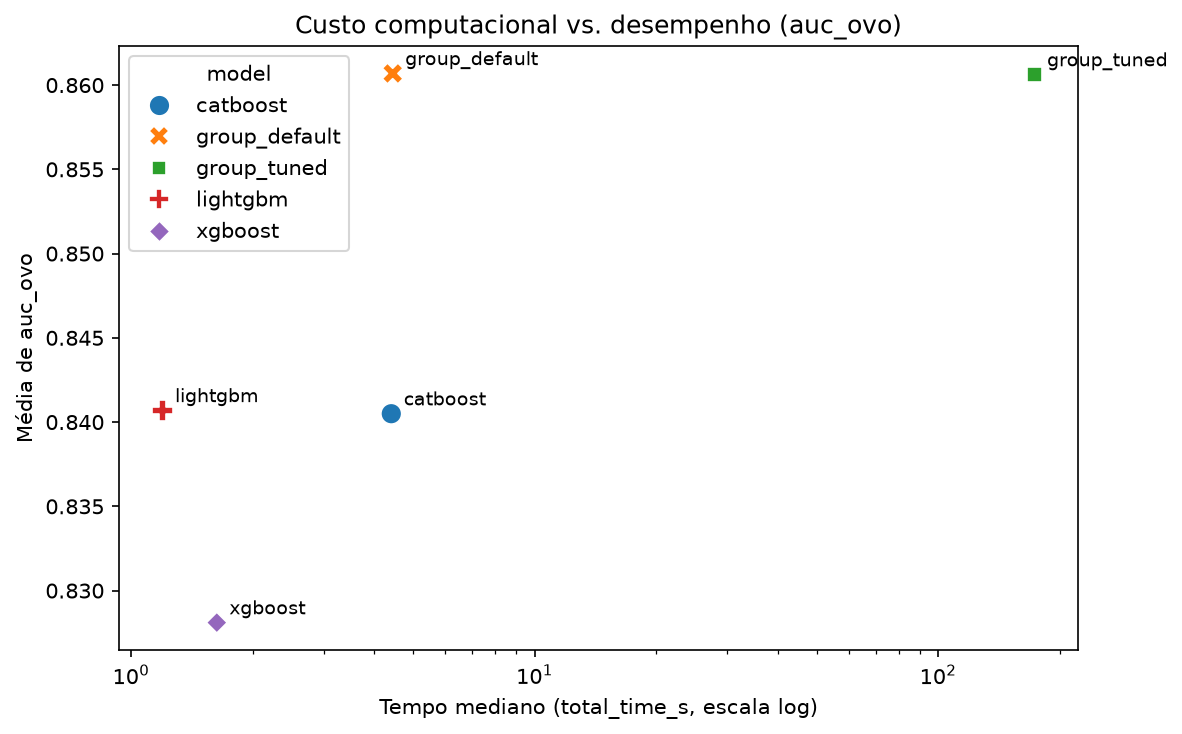
\includegraphics[width=0.76\textwidth]{../../../results/figures/custo_vs_desempenho.png}
    \caption{Compromisso entre tempo computacional total médio por fold externo (eixo horizontal) e desempenho preditivo médio em AUC OvO (eixo vertical) nos 30 datasets do conjunto de teste.}
    \label{fig:custo_desempenho}
\end{figure}

O gráfico permite identificar três faixas de compromisso entre custo e qualidade preditiva, sem pressupor que todos os sistemas citados pertençam à fronteira de Pareto:
\begin{enumerate}[leftmargin=2em]
    \item \textbf{Patamar de baixa latência (baselines GBDT, $3\text{ a }5\text{ s}$):} o \texttt{lightgbm} ($3{,}32\text{ s}$, AUC $0{,}8407$) apresenta AUC superior à do \texttt{xgboost} ($2{,}96\text{ s}$, AUC $0{,}8281$), mas também maior tempo médio; portanto, não o domina no sentido estrito de Pareto. Em relação ao \texttt{catboost} ($4{,}73\text{ s}$, AUC $0{,}8405$), o \texttt{lightgbm} combina AUC média ligeiramente maior e tempo menor;
    \item \textbf{Ponto ótimo de inferência em contexto sem busca (\texttt{group\_default}, $22{,}24\text{ s}$):} eleva a AUC OvO média para $0{,}8607$ ($+2{,}00\text{ p.p.}$) e atinge a menor entropia cruzada global ($0{,}3005$) sem custo de busca ($\texttt{tune\_time\_s} = 0$), concentrando seu tempo na inferência dos 8 Transformers sobre o contexto ($18{,}38\text{ s}$ em média, puxado pelas bases de $1.617$--$1.776$ colunas e testes de até $43.294$ linhas);
    \item \textbf{Custo elevado com retorno nulo da busca (\texttt{group\_tuned}, $218{,}78\text{ s}$):} multiplica o tempo total por $9{,}84\times$ devido aos $196{,}49\text{ s}$ médios da busca no Optuna sem produzir melhoria em AUC OvO ($0{,}8606$) e piorando a entropia cruzada ($0{,}3150$).
\end{enumerate}

\subsection{Respostas ao roteiro de análise}
\label{sec:respostas_nb04}

Consolidam-se a seguir as respostas às seis perguntas orientadoras do notebook \texttt{04\_analise\_estatistica.ipynb}:
\begin{enumerate}[leftmargin=2em]
    \item \textbf{Pergunta 1 (Rejeição em Friedman, uso de $F_F$ vs. $\chi^2_F$ e regra de completude):} sim, a hipótese nula do teste de Friedman é rejeitada a $5\%$ tanto por $\chi^2_F = 37{,}480$ ($p = 3{,}64 \times 10^{-8}$) quanto por $F_F = 20{,}695$ ($p = 3{,}28 \times 10^{-10}$). A decisão apoia-se em $F_F$ porque, conforme Demšar \cite{demsar2006statistical} (Seção 3.2.2), a aproximação qui-quadrado original de Friedman é excessivamente conservadora para valores moderados de $N$ e $k$, enquanto a estatística $F_F$ de Iman-Davenport (com distribuição $F$ de $(k-1)$ e $(k-1)(N-1)$ graus de liberdade) possui maior poder estatístico e calibração mais exata do erro Tipo~I. Nenhum dataset ficou de fora pela regra de completude ($N = 30$ completos);
    \item \textbf{Pergunta 2 (Diferenças contra baselines, Holm vs. Bonferroni-Dunn e poder estatístico):} \texttt{group\_tuned} supera significativamente todos os três baselines (LightGBM, CatBoost e XGBoost) a $5\%$. As conclusões por Holm e por Bonferroni-Dunn coincidem integralmente na AUC OvO porque a menor diferença de postos ($1{,}333$ contra LightGBM) supera com folga a diferença crítica de Bonferroni-Dunn ($\mathrm{CD}_{\mathrm{BD}} = 0{,}798$). Segundo Demšar \cite{demsar2006statistical}, o procedimento step-down de Holm é uniformemente mais poderoso que Bonferroni-Dunn porque testa as hipóteses ordenadas contra limiares sequenciais $\alpha/(k-1), \alpha/(k-2), \dots, \alpha/1$, enquanto Bonferroni-Dunn aplica o limiar mais rígido $\alpha/(k-1)$ a todas as comparações;
    \item \textbf{Pergunta 3 (Comparações todos contra todos vs. controle e leitura de grupos sobrepostos no diagrama CD):} quando o objetivo científico é testar um modelo proposto contra $k-1$ baselines, testes todos contra todos como Nemenyi controlam o erro familiar sobre $k(k-1)/2 = 6$ pares em vez de $k-1 = 3$ comparações, inflando o valor crítico ($\mathrm{CD}_{\mathrm{Nem}} = 0{,}856 > \mathrm{CD}_{\mathrm{BD}} = 0{,}798$) e perdendo poder estatístico. Quando um sistema pertence simultaneamente a duas barras horizontais sobrepostas num diagrama CD, Demšar \cite{demsar2006statistical} adverte que barras de conexão não representam classes de equivalência transitivas: significa apenas que os dados experimentais ($N$ finito) são insuficientes para distinguir estatisticamente o algoritmo intermediário de ambos os extremos, embora os extremos difiram significativamente entre si;
    \item \textbf{Pergunta 4 (Efeito da busca de hiperparâmetros, comparação com validação interna e Wilcoxon vs. Friedman/Holm):} não; a busca não melhorou significativamente o modelo no teste em AUC OvO ($p = 0{,}3285$ no Wilcoxon pareado entre \texttt{group\_tuned} e \texttt{group\_default}) e não compensa o aumento de $9{,}84\times$ no tempo total ($218{,}78\text{ s}$ vs. $22{,}24\text{ s}$). O pequeno ganho aparente da validação interna ($+0{,}0014$) era fruto de otimismo de seleção. Nas comparações de \texttt{group\_tuned} contra os três baselines, o Wilcoxon com correção de Holm ($p_{\text{Holm}} \le 2{,}38 \times 10^{-6}$, Tabela~\ref{tab:holm_wilcoxon}) coincidiu com Friedman/Holm, mas Benavoli, Corani e Mangili \cite{benavoli2016should} ressaltam uma diferença conceitual central: em Friedman, o posto de A vs. B depende do desempenho dos demais algoritmos C e D incluídos no pool (violando a independência de alternativas irrelevantes), enquanto o Wilcoxon signed-ranks depende exclusivamente das magnitudes das diferenças pareadas entre A e B;
    \item \textbf{Pergunta 5 (Destaques por regime, caráter descritivo e relação custo-desempenho):} o modelo destaca-se de forma absoluta nos datasets pequenos (posto médio $1{,}00$), mantendo liderança menor nos médios ($1{,}30$) e grandes ($1{,}60$). A análise por regimes é apenas descritiva porque cada célula contém apenas $N_{\text{cel}} \in \{6, 10, 15, 24\}$ datasets (para $N = 10$, $\mathrm{CD}_{\mathrm{Nem}} = 1{,}483$) e testar múltiplos subgrupos sem correção inflaria a taxa de falsos positivos. Na relação custo-desempenho, o \texttt{lightgbm} oferece o melhor compromisso entre os modelos ultrarrápidos de CPU ($3{,}32\text{ s}$, AUC $0{,}8407$), enquanto o \texttt{group\_default} oferece o melhor compromisso quando se prioriza qualidade preditiva medida por AUC e entropia cruzada ($22{,}24\text{ s}$, AUC $0{,}8607$, entropia cruzada $0{,}3005$);
    \item \textbf{Pergunta 6 (Repetição das seções 2 a 5 na métrica secundária \texttt{cross\_entropy} e multiplicidade entre métricas):} na entropia cruzada (menor é melhor), o teste global de Friedman/Iman-Davenport também rejeita $H_0$ ($F_F = 24{,}970$, $p = 9{,}53 \times 10^{-12}$), com postos médios $R_{\texttt{group\_tuned}} = 1{,}433$, $R_{\texttt{lightgbm}} = 2{,}133$, $R_{\texttt{catboost}} = 3{,}133$ e $R_{\texttt{xgboost}} = 3{,}300$. Três mudanças importantes emergem em relação à AUC OvO: (a) a diferença de postos entre \texttt{group\_tuned} e \texttt{lightgbm} cai para $0{,}700$, sendo significativa por Holm ($p_{\text{Holm}} = 0{,}0357$) e por Wilcoxon ($p_{\text{Holm}} = 0{,}00073$), mas não por Bonferroni-Dunn ($0{,}700 < 0{,}798$) nem por Nemenyi ($0{,}700 < 0{,}856$), ilustrando empiricamente o maior poder de Holm; (b) pelo teste de Nemenyi, o \texttt{lightgbm} passa a superar significativamente \texttt{catboost} ($\Delta R = 1{,}000 > 0{,}856$) e \texttt{xgboost} ($\Delta R = 1{,}167 > 0{,}856$) em entropia cruzada; e (c) no Wilcoxon pareado entre as variantes do grupo, \texttt{group\_default} supera significativamente \texttt{group\_tuned} em 29 dos 30 datasets ($T = 1{,}0$, $p = 3{,}73 \times 10^{-9}$). Para tratar a multiplicidade entre métricas, preserva-se a hierarquia pré-declarada (AUC OvO como confirmatória primária e entropia cruzada como secundária complementar); sob uma correção de Bonferroni conservadora entre as duas famílias ($\alpha/2 = 0{,}025$), todas as comparações continuariam significativas exceto \texttt{group\_tuned} vs. \texttt{lightgbm} no pós-teste de postos de Holm na entropia cruzada ($p_{\text{Holm}} = 0{,}0357 > 0{,}025$).
\end{enumerate}

% =============================================================================
\section{Discussão}
\label{sec:discussao}

Os resultados empíricos obtidos na Etapa~2 conectam-se diretamente às propriedades arquiteturais e matemáticas do TabICL v2 detalhadas na Etapa~1. A superioridade consistente do TabICL v2 sobre LightGBM, CatBoost e XGBoost em AUC OvO ($p_{\text{Holm}} \le 6{,}33 \times 10^{-5}$), acurácia, G-Mean e entropia cruzada confirma a tese central de Qu et al. \cite{qu2025tabicl,qu2026tabiclv2}: um modelo fundacional pré-treinado via aprendizagem em contexto sobre um prior sintético rico (combinando Modelos Causais Estruturais, ativações racionais de Cauchy e kernels de Sobolev) incorpora um viés indutivo multimodal capaz de aproximar fronteiras de decisão suaves e oblíquas que árvores ortogonais aos eixos só conseguem representar mediante particionamento excessivo.

Essa diferença de viés indutivo explica por que o domínio do TabICL v2 foi absoluto no regime de datasets pequenos ($n < 2.500$, posto médio $1{,}00$ nos 10 datasets). Como evidenciado pelo estudo de sobreajuste na Seção~\ref{sec:overfitting}, Nos datasets pequenos analisados, XGBoost e CatBoost apresentaram lacunas treino-validação elevadas ($0{,}1585$ e $0{,}1313$) , compatíveis com maior sobreajuste nesse recorte, sem que o experimento isole seu mecanismo causal. Por contraste, no TabICL v2 os pesos dos estágios $\mathrm{TF}_{\mathrm{col}}$, $\mathrm{TF}_{\mathrm{row}}$ e $\mathrm{TF}_{\mathrm{icl}}$ permanecem congelados: a inferência opera como uma aproximação amortizada da distribuição preditiva posterior Bayesiana, integrando implicitamente sobre hipóteses compatíveis com o contexto de treino e, neste conjunto de datasets, apresentou lacunas de generalização menores, sem demonstrar isoladamente a causa dessa diferença.

No regime de datasets grandes ($n \ge 10.000$), embora o TabICL v2 tenha mantido a liderança descritiva (AUC média de $0{,}8450$ e posto médio $1{,}60$), a distância para o LightGBM ($0{,}8355$, posto $2{,}20$) reduziu-se substancialmente. Uma possível explicação é que o regime grande oferece amostras suficientes para que os GBDTs estimem divisões mais estáveis, mas esse mecanismo não foi testado diretamente. Além disso, os dois paradigmas foram avaliados sob o mesmo teto protocolar de subamostragem estratificada ($\texttt{MAX\_SAMPLES} = 10.000$), o que impede extrapolar os resultados para o uso integral de bases maiores. As falhas de memória observadas mostram que a execução não foi uniformemente confortável na GPU T4 e na RAM disponíveis.

Um dos achados mais relevantes do estudo foi a superioridade do \texttt{group\_default} sobre o \texttt{group\_tuned} na métrica secundária de entropia cruzada (29 vitórias em 30 bases, $p = 3{,}73 \times 10^{-9}$) aliada à ausência de diferença significativa na métrica primária AUC OvO ($0{,}8607$ vs. $0{,}8606$, $p = 0{,}3285$). Conforme demonstrado no estudo de sensibilidade da Seção~\ref{sec:sensibilidade}, a A análise de sensibilidade sugeriu menor variação da AUC OvO com a temperatura de softmax $\tau$ que da entropia cruzada; essa observação é descritiva e se restringe às configurações investigadas. Como a busca maximizou a AUC OvO, não tinha a entropia cruzada como objetivo direto. Isso pode explicar a divergência entre métricas, mas não foi realizado um teste causal isolando temperaturas ou composições do ensemble no resultado final. A menor entropia cruzada da configuração padrão indica melhor desempenho na métrica probabilística avaliada, sem comprovar, por si só, calibração formal. Sob este protocolo e nos datasets considerados, não se observou benefício em AUC que justificasse o custo da busca.

Por fim, o custo computacional observado delimita com clareza os cenários de aplicação prática. Enquanto o LightGBM resolve o ajuste e a predição de um fold externo em $3{,}32\text{ s}$ em CPU, o \texttt{group\_default} exige $22{,}24\text{ s}$ em GPU T4, com picos de mais de $120\text{ s}$ em tabelas de altíssima dimensionalidade ($m > 1.600$, nas quais a complexidade $\mathcal{O}(n m^2)$ do estágio $\mathrm{TF}_{\mathrm{row}}$ e o descarregamento em disco do Estágio~1 dominam o tempo). Assim, o TabICL v2 padrão é uma alternativa atraente quando o objetivo é obter AUC elevada e menor entropia cruzada no regime avaliado e há GPU disponível. O LightGBM constitui uma opção de menor custo médio e execução em CPU nos datasets estudados; a escolha para outras cargas de trabalho exige avaliação própria de latência e qualidade preditiva.

\subsection{Ameaças à validade}
\label{sec:ameacas}

Seguindo a taxonomia clássica de validade experimental, registram-se quatro ameaças principais à validade deste estudo:
\begin{enumerate}[leftmargin=2em]
    \item \textbf{Validade interna (assimetria de busca e retomadas de sessão):} os baselines GBDT não passaram por busca de hiperparâmetros por dataset ($\texttt{tune\_time\_s} = 0$), utilizando os \emph{Tuned Defaults} meta-otimizados do \texttt{pytabkit}. Embora a configuração \texttt{group\_default} (sem busca) também tenha alcançado AUC OvO média elevada ($0{,}8607$), isso não elimina todas as possíveis consequências da assimetria de ajuste: GBDTs ajustados por Optuna com o mesmo orçamento de 20 trials poderiam estreitar a diferença de desempenho. Adicionalmente, como as execuções no Google Colab sofreram retomadas via \texttt{--resume}, os tempos de parede registrados podem refletir pequenas variações de carga de E/S da instância virtual;
    \item \textbf{Validade de construto (teto de subamostragem e métrica de otimização):} o protocolo impõe um teto de $10.000$ amostras de treinamento externo (\texttt{stratified\_subsample}). No regime grande ($n$ até $129.880$), esse limite restringe o volume de dados visto pelos GBDTs (que escalariam linearmente em CPU para o dataset inteiro), de modo que as conclusões no regime grande referem-se ao desempenho com até $10.000$ exemplos de treino;
    \item \textbf{Validade de conclusão estatística (tamanho amostral nos estratos e correlação entre folds):} com $N = 30$ datasets, os testes globais (Friedman, Iman-Davenport, Holm e Wilcoxon) possuem alto poder para detectar diferenças moderadas e grandes, mas as análises estratificadas por regime ($N_{\text{cel}} \in \{6, 10, 15\}$) carecem de potência estatística para inferência formal. Ademais, na seleção por regra de 1 EP (Seção~\ref{sec:overfitting}), o erro padrão calculado sobre $K = 3$ folds internos tem apenas 2 graus de liberdade e partições de treino parcialmente sobrepostas;
    \item \textbf{Validade externa (generalização além da suíte TabArena-v0.1):} embora os 30 datasets selecionados cubram ampla diversidade de domínios, tamanhos e proporções categóricas, todos pertencem à suíte curada TabArena-v0.1. A extrapolação direta para tabelas industriais com milhões de linhas, milhares de atributos esparsos ou forte deriva temporal (\emph{concept drift}) não é garantida sem validação específica.
\end{enumerate}

% =============================================================================
\section{Reprodutibilidade}
\label{sec:reprodutibilidade}

Todo o código-fonte, os testes automatizados, o protocolo congelado e os resultados consolidados estão registrados no repositório Git do grupo (\url{https://github.com/leticialevleitao/projetoAM20262Q2}). A reprodução do ambiente utiliza \texttt{uv}, os arquivos \texttt{pyproject.toml} e \texttt{uv.lock} e Python~3.12, além das dependências para TabICL, PyTorch, \texttt{pytabkit}, \texttt{scikit-learn}, Optuna e SciPy.

\paragraph{Hardware e tempos de execução.}
A validação interna e a maior parte da avaliação final foram executadas em Google Colab com GPU \textbf{NVIDIA Tesla T4} ($15.360\text{ MiB}$ de VRAM, driver \texttt{580.82.07}, Python~3.12). Duas avaliações finais com erro de memória foram recuperadas no \textbf{Kaggle}, com o mesmo arquivo de protocolo e o histórico de resultados preservado. Os dados não permitem atribuir toda a execução a uma única configuração de RAM ou a um único provedor. Na validação interna ($1.350$ registros válidos), os tempos medianos de ajuste e predição, em segundos, foram $0{,}640/0{,}036$ para LightGBM, $1{,}359/0{,}027$ para XGBoost, $2{,}536/0{,}026$ para CatBoost e $0{,}952/2{,}144$ para \texttt{group\_default}; a busca de \texttt{group\_tuned} teve mediana de $166{,}12\text{ s}$ por fold externo. Na avaliação final, a soma de \texttt{total\_time\_s} das $450$ combinações bem-sucedidas é de \textbf{$22.682{,}86\text{ s}$ ($6{,}30\text{ h}$)}, enquanto o intervalo cronológico entre o primeiro \texttt{inicio} e o último \texttt{fim} de \texttt{test\_log.csv} é de aproximadamente \textbf{$8{,}70\text{ h}$}. A primeira medida soma tempos instrumentados por avaliação; a segunda inclui interrupções, retomadas e intervalos entre sessões. Não devem ser confundidas.

\paragraph{Auditoria do protocolo (\texttt{check\_protocol}) e rastreabilidade.}
O arquivo \texttt{results/protocolo.lock} foi gerado em \texttt{2026-11-07T16:35:09+00:00}, a partir da árvore limpa identificada pelo commit \texttt{0595782fc4ae3d59e4805d38205ce5e9c2b79d5b}, e possui SHA-256 iniciado por \texttt{59901430bd8c} (valor integral no Apêndice~\ref{app:protocolo}). O lock foi registrado no commit \texttt{9718c9649b}, anterior à avaliação final. O primeiro commit com os resultados de teste é \texttt{983c42aa4f}. Em auditoria realizada sobre o estado do repositório incluído no pacote (HEAD \texttt{dd8ce5c}), \texttt{python -m src.pipeline.check\_protocol} retornou \textbf{APROVADO}: 30 arquivos protegidos conferidos nos commits pertinentes, uma execução inicial e quatro retomadas, retomadas restritas a combinações pendentes ou com erro, continuidade do lock no histórico e consistência de \texttt{test.csv} com os hashes do manifesto. O resumo literal da saída está no Apêndice~\ref{app:protocolo}.

\paragraph{Comandos para reprodução completa.}
\begin{verbatim}
# 1. Instalar dependencias e pacote extra do modelo tema (TabICL v2)
uv sync --extra dev --extra tabicl

# 2. Verificar selecao dos 30 datasets e suite estrita de testes unitarios
uv run python -m src.pipeline.check_selection
AM_STRICT=1 uv run pytest

# 3. Fase de desenvolvimento (validacao cruzada interna)
uv run python -m src.pipeline.run_validation --resume

# 4. Conferir a integridade do experimento ja concluido
uv run python -m src.pipeline.check_protocol

# 5. Consultar os notebooks de analise de resultados
# notebooks/04_analise_estatistica.ipynb
# notebooks/05_overfitting.ipynb
\end{verbatim}

% =============================================================================
\begin{thebibliography}{99}

\bibitem{benavoli2016should}
A.~Benavoli, G.~Corani, and F.~Mangili.
\newblock Should we really use post-hoc tests based on mean-ranks?
\newblock \emph{Journal of Machine Learning Research}, 17(5):1--10, 2016.

\bibitem{breiman1984classification}
L.~Breiman, J.~Friedman, C.~J. Stone, and R.~A. Olshen.
\newblock \emph{Classification and Regression Trees}.
\newblock Wadsworth and Brooks, Monterey, CA, 1984.

\bibitem{cawley2010overfitting}
G.~C. Cawley and N.~L.~C. Talbot.
\newblock On over-fitting in model selection and subsequent selection bias in performance evaluation.
\newblock \emph{Journal of Machine Learning Research}, 11:2079--2107, 2010.

\bibitem{chen2016xgboost}
T.~Chen and C.~Guestrin.
\newblock {XGBoost}: A scalable tree boosting system.
\newblock In \emph{Proceedings of the 22nd ACM SIGKDD International Conference on Knowledge Discovery and Data Mining}, pages 785--794, 2016.

\bibitem{demsar2006statistical}
J.~Dem\v{s}ar.
\newblock Statistical comparisons of classifiers over multiple data sets.
\newblock \emph{Journal of Machine Learning Research}, 7:1--30, 2006.

\bibitem{erickson2025tabarena}
N.~Erickson, D.~Holzm\"{u}ller, L.~Grinsztajn, et~al.
\newblock {TabArena}: A living benchmark for machine learning on tabular data.
\newblock \emph{arXiv preprint arXiv:2506.16791}, 2025.

\bibitem{gorishniy2021revisiting}
Y.~Gorishniy, I.~Rubachev, V.~Khrulkov, and A.~Babenko.
\newblock Revisiting deep learning models for tabular data.
\newblock In \emph{Advances in Neural Information Processing Systems (NeurIPS)}, volume~34, pages 18932--18943, 2021.

\bibitem{gorishniy2022embeddings}
Y.~Gorishniy, I.~Rubachev, and A.~Babenko.
\newblock On embeddings for numerical features in tabular deep learning.
\newblock In \emph{Advances in Neural Information Processing Systems (NeurIPS)}, volume~35, pages 24991--25004, 2022.

\bibitem{gorishniy2024tabr}
Y.~Gorishniy, I.~Rubachev, N.~Kartashev, D.~Shlenskii, A.~Kotelnikov, and A.~Babenko.
\newblock {TabR}: Tabular deep learning meets nearest neighbors.
\newblock In \emph{International Conference on Learning Representations (ICLR)}, 2024.

\bibitem{gorishniy2025tabm}
Y.~Gorishniy, A.~Kotelnikov, and A.~Babenko.
\newblock {TabM}: Advancing tabular deep learning with parameter-efficient ensembling.
\newblock In \emph{International Conference on Learning Representations (ICLR)}, 2025.

\bibitem{grinsztajn2022tree}
L.~Grinsztajn, E.~Oyallon, and G.~Varoquaux.
\newblock Why do tree-based models still outperform deep learning on typical tabular data?
\newblock In \emph{Advances in Neural Information Processing Systems (NeurIPS)}, volume~35, pages 507--520, 2022.

\bibitem{hastie2009elements}
T.~Hastie, R.~Tibshirani, and J.~Friedman.
\newblock \emph{The Elements of Statistical Learning: Data Mining, Inference, and Prediction}.
\newblock Springer, 2nd edition, 2009.

\bibitem{hollmann2023tabpfn}
N.~Hollmann, S.~M\"{u}ller, K.~Eggensperger, and F.~Hutter.
\newblock {TabPFN}: A transformer that solves small tabular classification problems in a second.
\newblock In \emph{International Conference on Learning Representations (ICLR)}, 2023.

\bibitem{hollmann2025tabpfn}
N.~Hollmann, S.~M\"{u}ller, L.~Purucker, A.~Krishnakumar, M.~K\"{o}rfer, S.~B. Hoo, R.~T. Schirrmeister, and F.~Hutter.
\newblock Accurate predictions on small data with a tabular foundation model.
\newblock \emph{Nature}, 637:319--326, 2025.

\bibitem{holzmuller2024better}
D.~Holzm\"{u}ller, L.~Grinsztajn, and I.~Steinwart.
\newblock Better by default: Strong pre-tuned {MLPs} and boosted trees on tabular data.
\newblock In \emph{Advances in Neural Information Processing Systems (NeurIPS)}, volume~37, 2024.

\bibitem{jordan2024muon}
K.~Jordan, Y.~Jin, V.~Boza, J.~You, F.~Cesista, L.~Newhouse, and J.~Bernstein.
\newblock {Muon}: An optimizer for hidden layers in neural networks, 2024.

\bibitem{ke2017lightgbm}
G.~Ke, Q.~Meng, T.~Finley, T.~Wang, W.~Chen, W.~Ma, Q.~Ye, and T.-Y. Liu.
\newblock {LightGBM}: A highly efficient gradient boosting decision tree.
\newblock In \emph{Advances in Neural Information Processing Systems (NeurIPS)}, volume~30, pages 3146--3154, 2017.

\bibitem{lee2019set}
J.~Lee, Y.~Lee, J.~Kim, A.~Kosiorek, S.~Choi, and Y.~W. Teh.
\newblock Set transformer: A framework for attention-based permutation-invariant neural networks.
\newblock In \emph{Proceedings of the 36th International Conference on Machine Learning (ICML)}, pages 3744--3753, 2019.

\bibitem{mcelfresh2023when}
D.~McElfresh, S.~Khandagale, J.~Valverde, V.~Prasad~C, G.~Ramakrishnan, M.~Goldblum, and C.~White.
\newblock When do neural nets outperform boosted trees on tabular data?
\newblock In \emph{Advances in Neural Information Processing Systems (NeurIPS)}, volume~36, 2023.

\bibitem{prokhorenkova2018catboost}
L.~Prokhorenkova, G.~Gusev, A.~Vorobev, A.~V. Dorogush, and A.~Gulin.
\newblock {CatBoost}: unbiased boosting with categorical features.
\newblock In \emph{Advances in Neural Information Processing Systems (NeurIPS)}, volume~31, pages 6638--6648, 2018.

\bibitem{qu2025tabicl}
J.~Qu, D.~Holzm\"{u}ller, G.~Varoquaux, and M.~Le~Morvan.
\newblock {TabICL}: A tabular foundation model for in-context learning on large data.
\newblock In \emph{Proceedings of the 42nd International Conference on Machine Learning (ICML)}, 2025.

\bibitem{qu2026tabiclv2}
J.~Qu, D.~Holzm\"{u}ller, G.~Varoquaux, and M.~Le~Morvan.
\newblock {TabICLv2}: A better, faster, scalable, and open tabular foundation model.
\newblock \emph{arXiv preprint arXiv:2602.11139v2}, 2026.

\bibitem{varma2006bias}
S.~Varma and R.~Simon.
\newblock Bias in error estimation when using cross-validation for model selection.
\newblock \emph{BMC Bioinformatics}, 7(1):91, 2006.

\end{thebibliography}

\newpage
\appendix

% =============================================================================
\section{Tabela dos 30 datasets selecionados}
\label{app:datasets}

A Tabela~\ref{tab:app_datasets} apresenta a relação completa dos 30 datasets selecionados da suíte TabArena-v0.1 (\texttt{data/selecao\_datasets.txt} e \texttt{results/tabela\_datasets.md}), ordenados por regime de tamanho e número de amostras.

\begin{table}[htbp]
    \centering
    \caption{Catálogo completo dos 30 datasets selecionados na suíte TabArena-v0.1 ($10$ pequenos, $10$ médios e $10$ grandes).}
    \label{tab:app_datasets}
    \footnotesize
    \resizebox{\textwidth}{!}{%
    \begin{tabular}{@{}rlrrrlrrl@{}}
        \toprule
        \textbf{Task ID} & \textbf{Nome do dataset} & $n$ & $m$ & $C$ & \textbf{\% Categ.} & \textbf{Ausentes} & \textbf{Razão desb.} & \textbf{Regime} \\
        \midrule
        363621 & blood-transfusion-service-center & 748 & 4 & 2 & 0,0\% & Não & 3,20 & small \\
        363629 & diabetes & 768 & 8 & 2 & 0,0\% & Não & 1,87 & small \\
        363626 & credit-g & 1.000 & 20 & 2 & 65,0\% & Não & 2,33 & small \\
        363685 & maternal\_health\_risk & 1.014 & 6 & 3 & 0,0\% & Não & 1,49 & small \\
        363696 & qsar-biodeg & 1.054 & 41 & 2 & 12,2\% & Não & 1,97 & small \\
        363707 & website\_phishing & 1.353 & 9 & 3 & 100,0\% & Não & 6,82 & small \\
        363671 & Fitness\_Club & 1.500 & 6 & 2 & 50,0\% & Sim & 2,30 & small \\
        363682 & Is-this-a-good-customer & 1.723 & 13 & 2 & 61,5\% & Não & 7,79 & small \\
        363684 & Marketing\_Campaign & 2.240 & 25 & 2 & 32,0\% & Sim & 5,71 & small \\
        363674 & hazelnut-spread-contaminant-detection & 2.400 & 30 & 2 & 0,0\% & Não & 1,00 & small \\
        \midrule
        363700 & seismic-bumps & 2.584 & 15 & 2 & 20,0\% & Não & 14,20 & medium \\
        363702 & splice & 3.190 & 60 & 3 & 100,0\% & Não & 2,16 & medium \\
        363620 & Bioresponse & 3.751 & 1776 & 2 & 0,0\% & Não & 1,18 & medium \\
        363677 & hiva\_agnostic & 3.845 & 1617 & 3 & 100,0\% & Não & 88,33 & medium \\
        363704 & students\_dropout\_and\_academic\_success & 4.424 & 36 & 3 & 47,2\% & Não & 2,78 & medium \\
        363623 & churn & 5.000 & 19 & 2 & 21,1\% & Não & 6,07 & medium \\
        363694 & polish\_companies\_bankruptcy & 5.910 & 64 & 2 & 0,0\% & Sim & 13,41 & medium \\
        363706 & taiwanese\_bankruptcy\_prediction & 6.819 & 94 & 2 & 0,0\% & Não & 30,00 & medium \\
        363689 & NATICUSdroid & 7.491 & 86 & 2 & 100,0\% & Não & 1,85 & medium \\
        363624 & coil2000\_insurance\_policies & 9.822 & 85 & 2 & 3,5\% & Não & 15,76 & medium \\
        \midrule
        363676 & heloc & 10.459 & 23 & 2 & 0,0\% & Não & 1,09 & large \\
        363712 & jm1 & 10.885 & 21 & 2 & 0,0\% & Sim & 4,17 & large \\
        363632 & E-CommereShippingData & 10.999 & 10 & 2 & 40,0\% & Não & 1,48 & large \\
        363691 & online\_shoppers\_intention & 12.330 & 17 & 2 & 41,2\% & Não & 5,46 & large \\
        363681 & in\_vehicle\_coupon\_recommendation & 12.684 & 24 & 2 & 87,5\% & Não & 1,32 & large \\
        363679 & HR\_Analytics\_Job\_Change\_of\_Data\_Scientists & 19.158 & 12 & 2 & 75,0\% & Sim & 3,01 & large \\
        363627 & credit\_card\_clients\_default & 30.000 & 23 & 2 & 13,0\% & Não & 3,52 & large \\
        363618 & bank-marketing & 45.211 & 13 & 2 & 53,8\% & Não & 7,55 & large \\
        363699 & SDSS17 & 78.053 & 11 & 3 & 18,2\% & Não & 3,40 & large \\
        363628 & customer\_satisfaction\_in\_airline & 129.880 & 21 & 2 & 76,2\% & Sim & 1,21 & large \\
        \bottomrule
    \end{tabular}
    }%
\end{table}

% =============================================================================
\section{Espaço de busca e histórico do Optuna}
\label{app:optuna}

A implementação exata de \texttt{search\_space(trial)} congelada em \texttt{src/models/group\_model.py} e auditada em \texttt{results/protocolo.lock} define:
\begin{verbatim}
NORM_METHODS_MAP = {
    "none+power": ["none", "power"],
    "none+power+robust": ["none", "power", "robust"],
    "none+power+quantile_rtdl": ["none", "power", "quantile_rtdl"],
    "power": ["power"],
    "quantile_rtdl": ["quantile_rtdl"],
}

def search_space(trial) -> dict[str, Any]:
    norm_key = trial.suggest_categorical(
        "norm_methods", list(NORM_METHODS_MAP.keys()))
    return {
        "norm_methods": NORM_METHODS_MAP[norm_key],
        "outlier_threshold": trial.suggest_float(
            "outlier_threshold", 2.5, 6.0, log=False),
        "softmax_temperature": trial.suggest_float(
            "softmax_temperature", 0.5, 1.5, log=True),
        "average_logits": trial.suggest_categorical(
            "average_logits", [True, False]),
    }
\end{verbatim}

Na execução das $90$ buscas independentes do Optuna ($30\text{ datasets} \times 3\text{ folds externos}$, semente do amostrador TPE $\texttt{seed} = 42 + \text{fold}$, orçamento de $\texttt{n\_trials} = 20$ e $\texttt{timeout} = 600\text{ s}$), o tempo de busca no conjunto de teste teve média de $196{,}49 \pm 160{,}79\text{ s}$ (mediana de $166{,}12\text{ s}$ na validação interna, variando de $40{,}61\text{ s}$ em \texttt{blood-transfusion-service-center} até $679{,}56\text{ s}$ em \texttt{hiva\_agnostic}, onde o limite de $600\text{ s}$ interrompeu a busca após a conclusão do trial em andamento). No estudo de demonstração do notebook \texttt{03\_demo\_modelo\_grupo.ipynb} (treino do fold 0 de \texttt{363621}), a melhor configuração encontrada pelo Optuna atingiu AUC OvO interna de $0{,}7568$ com $\texttt{norm\_methods} = \texttt{["none", "power", "quantile\_rtdl"]}$, $\texttt{outlier\_threshold} = 4{,}873$, $\texttt{softmax\_temperature} = 0{,}602$ e $\texttt{average\_logits} = \texttt{False}$.

% =============================================================================
\section{Resultados por dataset}
\label{app:por_dataset}

As Tabelas~\ref{tab:app_auc_dataset} e~\ref{tab:app_ce_dataset} reportam as médias e desvios-padrão sobre os 3 folds externos de teste (\texttt{per\_dataset\_table}) para os 30 datasets na métrica primária (AUC OvO) e na métrica secundária (entropia cruzada).

\begin{table}[htbp]
    \centering
    \caption{Resultados por dataset na métrica primária \textbf{AUC OvO} (média $\pm$ desvio-padrão nos 3 folds externos de teste; maior é melhor).}
    \label{tab:app_auc_dataset}
    \resizebox{\textwidth}{!}{%
    \begin{tabular}{@{}lrrrrr@{}}
        \toprule
        \textbf{Dataset} & \texttt{group\_default} & \texttt{group\_tuned} & \texttt{lightgbm} & \texttt{catboost} & \texttt{xgboost} \\
        \midrule
        Bioresponse & 0,8594 $\pm$ 0,0110 & 0,8622 $\pm$ 0,0104 & 0,8550 $\pm$ 0,0241 & 0,8600 $\pm$ 0,0170 & 0,8541 $\pm$ 0,0232 \\
        E-CommereShippingData & 0,7440 $\pm$ 0,0035 & 0,7434 $\pm$ 0,0033 & 0,7449 $\pm$ 0,0053 & 0,7443 $\pm$ 0,0073 & 0,7439 $\pm$ 0,0022 \\
        Fitness\_Club & 0,8218 $\pm$ 0,0121 & 0,8223 $\pm$ 0,0123 & 0,8032 $\pm$ 0,0030 & 0,7951 $\pm$ 0,0136 & 0,7999 $\pm$ 0,0115 \\
        HR\_Analytics\_Job\_Change\_of\_Data\_Scientists & 0,8067 $\pm$ 0,0087 & 0,8067 $\pm$ 0,0088 & 0,8001 $\pm$ 0,0063 & 0,7971 $\pm$ 0,0050 & 0,7901 $\pm$ 0,0074 \\
        Is-this-a-good-customer & 0,7488 $\pm$ 0,0150 & 0,7471 $\pm$ 0,0136 & 0,6666 $\pm$ 0,0652 & 0,6861 $\pm$ 0,0491 & 0,6939 $\pm$ 0,0183 \\
        Marketing\_Campaign & 0,9140 $\pm$ 0,0200 & 0,9144 $\pm$ 0,0199 & 0,8824 $\pm$ 0,0271 & 0,8524 $\pm$ 0,0127 & 0,6060 $\pm$ 0,0678 \\
        NATICUSdroid & 0,9879 $\pm$ 0,0008 & 0,9880 $\pm$ 0,0009 & 0,9830 $\pm$ 0,0018 & 0,9841 $\pm$ 0,0019 & 0,9840 $\pm$ 0,0015 \\
        SDSS17 & 0,9970 $\pm$ 0,0000 & 0,9972 $\pm$ 0,0001 & 0,9933 $\pm$ 0,0015 & 0,9742 $\pm$ 0,0010 & 0,9923 $\pm$ 0,0001 \\
        bank-marketing & 0,7620 $\pm$ 0,0120 & 0,7547 $\pm$ 0,0228 & 0,7600 $\pm$ 0,0089 & 0,7616 $\pm$ 0,0087 & 0,7569 $\pm$ 0,0111 \\
        blood-transfusion-service-center & 0,7522 $\pm$ 0,0429 & 0,7527 $\pm$ 0,0438 & 0,7231 $\pm$ 0,0505 & 0,7253 $\pm$ 0,0394 & 0,6854 $\pm$ 0,0625 \\
        churn & 0,9316 $\pm$ 0,0113 & 0,9323 $\pm$ 0,0112 & 0,9132 $\pm$ 0,0178 & 0,9191 $\pm$ 0,0109 & 0,8987 $\pm$ 0,0194 \\
        coil2000\_insurance\_policies & 0,7709 $\pm$ 0,0064 & 0,7712 $\pm$ 0,0065 & 0,6933 $\pm$ 0,0486 & 0,7364 $\pm$ 0,0214 & 0,7204 $\pm$ 0,0310 \\
        credit-g & 0,7922 $\pm$ 0,0183 & 0,7917 $\pm$ 0,0184 & 0,7489 $\pm$ 0,0252 & 0,7668 $\pm$ 0,0182 & 0,7554 $\pm$ 0,0202 \\
        credit\_card\_clients\_default & 0,7911 $\pm$ 0,0045 & 0,7908 $\pm$ 0,0048 & 0,7800 $\pm$ 0,0065 & 0,7795 $\pm$ 0,0087 & 0,7787 $\pm$ 0,0069 \\
        customer\_satisfaction\_in\_airline & 0,9953 $\pm$ 0,0002 & 0,9953 $\pm$ 0,0002 & 0,9939 $\pm$ 0,0003 & 0,9939 $\pm$ 0,0004 & 0,9936 $\pm$ 0,0003 \\
        diabetes & 0,8423 $\pm$ 0,0068 & 0,8425 $\pm$ 0,0093 & 0,8182 $\pm$ 0,0260 & 0,8181 $\pm$ 0,0086 & 0,8151 $\pm$ 0,0113 \\
        hazelnut-spread-contaminant-detection & 0,9943 $\pm$ 0,0031 & 0,9943 $\pm$ 0,0032 & 0,9723 $\pm$ 0,0021 & 0,9649 $\pm$ 0,0104 & 0,9696 $\pm$ 0,0041 \\
        heloc & 0,8023 $\pm$ 0,0045 & 0,8025 $\pm$ 0,0048 & 0,7898 $\pm$ 0,0096 & 0,7935 $\pm$ 0,0080 & 0,7890 $\pm$ 0,0068 \\
        hiva\_agnostic & 0,4683 $\pm$ 0,0194 & 0,4759 $\pm$ 0,0243 & 0,4944 $\pm$ 0,0193 & 0,4894 $\pm$ 0,0257 & 0,4985 $\pm$ 0,0549 \\
        in\_vehicle\_coupon\_recommendation & 0,8434 $\pm$ 0,0070 & 0,8427 $\pm$ 0,0078 & 0,8222 $\pm$ 0,0061 & 0,8216 $\pm$ 0,0044 & 0,8237 $\pm$ 0,0072 \\
        jm1 & 0,7759 $\pm$ 0,0100 & 0,7787 $\pm$ 0,0079 & 0,7399 $\pm$ 0,0178 & 0,7370 $\pm$ 0,0165 & 0,7370 $\pm$ 0,0099 \\
        maternal\_health\_risk & 0,9635 $\pm$ 0,0085 & 0,9636 $\pm$ 0,0079 & 0,9203 $\pm$ 0,0034 & 0,9351 $\pm$ 0,0043 & 0,9374 $\pm$ 0,0003 \\
        online\_shoppers\_intention & 0,9370 $\pm$ 0,0058 & 0,9378 $\pm$ 0,0046 & 0,9310 $\pm$ 0,0048 & 0,9290 $\pm$ 0,0062 & 0,9286 $\pm$ 0,0030 \\
        polish\_companies\_bankruptcy & 0,9837 $\pm$ 0,0036 & 0,9847 $\pm$ 0,0035 & 0,9488 $\pm$ 0,0122 & 0,9510 $\pm$ 0,0052 & 0,9437 $\pm$ 0,0083 \\
        qsar-biodeg & 0,9435 $\pm$ 0,0080 & 0,9439 $\pm$ 0,0083 & 0,9210 $\pm$ 0,0064 & 0,9271 $\pm$ 0,0072 & 0,9289 $\pm$ 0,0089 \\
        seismic-bumps & 0,7878 $\pm$ 0,0134 & 0,7787 $\pm$ 0,0198 & 0,7563 $\pm$ 0,0366 & 0,7385 $\pm$ 0,0256 & 0,6981 $\pm$ 0,0213 \\
        splice & 0,9961 $\pm$ 0,0016 & 0,9960 $\pm$ 0,0016 & 0,9945 $\pm$ 0,0013 & 0,9930 $\pm$ 0,0025 & 0,9952 $\pm$ 0,0015 \\
        students\_dropout\_and\_academic\_success & 0,8858 $\pm$ 0,0089 & 0,8856 $\pm$ 0,0081 & 0,8715 $\pm$ 0,0084 & 0,8540 $\pm$ 0,0257 & 0,8668 $\pm$ 0,0078 \\
        taiwanese\_bankruptcy\_prediction & 0,9432 $\pm$ 0,0027 & 0,9429 $\pm$ 0,0036 & 0,9325 $\pm$ 0,0165 & 0,9261 $\pm$ 0,0072 & 0,8912 $\pm$ 0,0583 \\
        website\_phishing & 0,9785 $\pm$ 0,0013 & 0,9788 $\pm$ 0,0010 & 0,9672 $\pm$ 0,0050 & 0,9606 $\pm$ 0,0121 & 0,9668 $\pm$ 0,0030 \\
        \bottomrule
    \end{tabular}%
    }
\end{table}

\begin{table}[htbp]
    \centering
    \caption{Resultados por dataset na métrica secundária \textbf{entropia cruzada} (\texttt{cross\_entropy}, média $\pm$ desvio-padrão nos 3 folds externos de teste; menor é melhor).}
    \label{tab:app_ce_dataset}
    \resizebox{\textwidth}{!}{%
    \begin{tabular}{@{}lrrrrr@{}}
        \toprule
        \textbf{Dataset} & \texttt{group\_default} & \texttt{group\_tuned} & \texttt{lightgbm} & \texttt{catboost} & \texttt{xgboost} \\
        \midrule
        Bioresponse & 0,4733 $\pm$ 0,0154 & 0,5455 $\pm$ 0,0217 & 0,4990 $\pm$ 0,0536 & 0,4699 $\pm$ 0,0257 & 0,4928 $\pm$ 0,0448 \\
        E-CommereShippingData & 0,4969 $\pm$ 0,0030 & 0,5002 $\pm$ 0,0065 & 0,5125 $\pm$ 0,0030 & 0,6551 $\pm$ 0,0273 & 0,5130 $\pm$ 0,0021 \\
        Fitness\_Club & 0,4634 $\pm$ 0,0149 & 0,4928 $\pm$ 0,0504 & 0,4841 $\pm$ 0,0023 & 0,5356 $\pm$ 0,0480 & 0,4930 $\pm$ 0,0161 \\
        HR\_Analytics\_Job\_Change\_of\_Data\_Scientists & 0,4338 $\pm$ 0,0103 & 0,4669 $\pm$ 0,0539 & 0,4395 $\pm$ 0,0054 & 0,5122 $\pm$ 0,1023 & 0,4542 $\pm$ 0,0135 \\
        Is-this-a-good-customer & 0,3168 $\pm$ 0,0059 & 0,3354 $\pm$ 0,0267 & 0,3517 $\pm$ 0,0023 & 0,4515 $\pm$ 0,1162 & 0,4814 $\pm$ 0,2584 \\
        Marketing\_Campaign & 0,2507 $\pm$ 0,0309 & 0,2573 $\pm$ 0,0281 & 0,3279 $\pm$ 0,0473 & 0,4016 $\pm$ 0,1029 & 0,4333 $\pm$ 0,0096 \\
        NATICUSdroid & 0,1328 $\pm$ 0,0053 & 0,1354 $\pm$ 0,0016 & 0,1616 $\pm$ 0,0117 & 0,1543 $\pm$ 0,0107 & 0,1537 $\pm$ 0,0070 \\
        SDSS17 & 0,0718 $\pm$ 0,0017 & 0,0804 $\pm$ 0,0016 & 0,1285 $\pm$ 0,0262 & 0,9140 $\pm$ 0,0933 & 0,1402 $\pm$ 0,0077 \\
        bank-marketing & 0,3041 $\pm$ 0,0044 & 0,3097 $\pm$ 0,0050 & 0,3052 $\pm$ 0,0023 & 0,3035 $\pm$ 0,0022 & 0,3064 $\pm$ 0,0035 \\
        blood-transfusion-service-center & 0,4721 $\pm$ 0,0257 & 0,4764 $\pm$ 0,0289 & 0,4984 $\pm$ 0,0385 & 0,5716 $\pm$ 0,0776 & 0,8902 $\pm$ 0,6603 \\
        churn & 0,1189 $\pm$ 0,0110 & 0,1249 $\pm$ 0,0095 & 0,2045 $\pm$ 0,0186 & 0,1727 $\pm$ 0,0143 & 0,2441 $\pm$ 0,0480 \\
        coil2000\_insurance\_policies & 0,1995 $\pm$ 0,0013 & 0,2108 $\pm$ 0,0136 & 0,2173 $\pm$ 0,0114 & 0,2688 $\pm$ 0,0766 & 0,2151 $\pm$ 0,0036 \\
        credit-g & 0,4945 $\pm$ 0,0226 & 0,4932 $\pm$ 0,0156 & 0,5345 $\pm$ 0,0129 & 0,6754 $\pm$ 0,1927 & 0,6335 $\pm$ 0,0895 \\
        credit\_card\_clients\_default & 0,4234 $\pm$ 0,0045 & 0,4309 $\pm$ 0,0125 & 0,4305 $\pm$ 0,0027 & 0,4487 $\pm$ 0,0361 & 0,4317 $\pm$ 0,0025 \\
        customer\_satisfaction\_in\_airline & 0,0839 $\pm$ 0,0025 & 0,0867 $\pm$ 0,0060 & 0,0984 $\pm$ 0,0022 & 0,0992 $\pm$ 0,0045 & 0,1019 $\pm$ 0,0045 \\
        diabetes & 0,4631 $\pm$ 0,0063 & 0,4691 $\pm$ 0,0128 & 0,5031 $\pm$ 0,0413 & 0,5507 $\pm$ 0,0496 & 0,7181 $\pm$ 0,2784 \\
        hazelnut-spread-contaminant-detection & 0,0916 $\pm$ 0,0241 & 0,0947 $\pm$ 0,0309 & 0,2458 $\pm$ 0,0247 & 0,3363 $\pm$ 0,0683 & 0,4473 $\pm$ 0,1247 \\
        heloc & 0,5417 $\pm$ 0,0056 & 0,5444 $\pm$ 0,0055 & 0,5603 $\pm$ 0,0126 & 0,5536 $\pm$ 0,0098 & 0,5592 $\pm$ 0,0103 \\
        hiva\_agnostic & 0,2075 $\pm$ 0,0103 & 0,2528 $\pm$ 0,0414 & 0,2340 $\pm$ 0,1039 & 1,0137 $\pm$ 0,1295 & 0,2722 $\pm$ 0,1056 \\
        in\_vehicle\_coupon\_recommendation & 0,4833 $\pm$ 0,0086 & 0,4856 $\pm$ 0,0114 & 0,5253 $\pm$ 0,0177 & 0,5237 $\pm$ 0,0055 & 0,5443 $\pm$ 0,0488 \\
        jm1 & 0,4123 $\pm$ 0,0018 & 0,4263 $\pm$ 0,0083 & 0,4316 $\pm$ 0,0086 & 0,4368 $\pm$ 0,0128 & 0,4379 $\pm$ 0,0087 \\
        maternal\_health\_risk & 0,3605 $\pm$ 0,0329 & 0,3741 $\pm$ 0,0470 & 0,5353 $\pm$ 0,0207 & 0,5413 $\pm$ 0,0892 & 0,8750 $\pm$ 0,2115 \\
        online\_shoppers\_intention & 0,2172 $\pm$ 0,0093 & 0,2288 $\pm$ 0,0060 & 0,2293 $\pm$ 0,0081 & 0,3494 $\pm$ 0,1744 & 0,2380 $\pm$ 0,0037 \\
        polish\_companies\_bankruptcy & 0,0656 $\pm$ 0,0071 & 0,0727 $\pm$ 0,0141 & 0,1272 $\pm$ 0,0120 & 0,1290 $\pm$ 0,0193 & 0,2550 $\pm$ 0,0841 \\
        qsar-biodeg & 0,2862 $\pm$ 0,0196 & 0,2920 $\pm$ 0,0135 & 0,3452 $\pm$ 0,0090 & 0,3867 $\pm$ 0,0774 & 0,5862 $\pm$ 0,2262 \\
        seismic-bumps & 0,2072 $\pm$ 0,0047 & 0,2382 $\pm$ 0,0335 & 0,2230 $\pm$ 0,0137 & 0,2454 $\pm$ 0,0212 & 0,4825 $\pm$ 0,0801 \\
        splice & 0,0984 $\pm$ 0,0265 & 0,1210 $\pm$ 0,0319 & 0,1201 $\pm$ 0,0223 & 0,1610 $\pm$ 0,0606 & 0,1966 $\pm$ 0,0292 \\
        students\_dropout\_and\_academic\_success & 0,5346 $\pm$ 0,0194 & 0,5758 $\pm$ 0,0306 & 0,6429 $\pm$ 0,1134 & 1,1730 $\pm$ 1,0328 & 0,7246 $\pm$ 0,2097 \\
        taiwanese\_bankruptcy\_prediction & 0,0831 $\pm$ 0,0037 & 0,0908 $\pm$ 0,0102 & 0,1463 $\pm$ 0,0869 & 0,1273 $\pm$ 0,0185 & 0,1227 $\pm$ 0,0078 \\
        website\_phishing & 0,2282 $\pm$ 0,0226 & 0,2364 $\pm$ 0,0221 & 0,2786 $\pm$ 0,0225 & 0,4902 $\pm$ 0,2803 & 0,3879 $\pm$ 0,1219 \\
        \bottomrule
    \end{tabular}%
    }
\end{table}

% =============================================================================
\section{Registro do protocolo}
\label{app:protocolo}

Apresentam-se os registros efetivos conferidos no repositório Git e em \texttt{results/test\_log.csv}, sem substituir os logs originais.

\paragraph{1. Commits e integridade do protocolo.}
\begin{itemize}[leftmargin=2em]
    \item Seleção inicial de datasets: \texttt{1db4ff8}; declarações a priori e modelo do grupo: \texttt{0a99b2c}, atualizados em \texttt{e2c6968};
    \item Commit da árvore de desenvolvimento congelada, registrado dentro do lock: \texttt{0595782fc4ae3d59e4805d38205ce5e9c2b79d5b};
    \item Commit de \texttt{results/protocolo.lock}: \texttt{9718c9649b};
    \item Primeiro commit com resultados da avaliação final: \texttt{983c42aa4f};
    \item Estado do repositório auditado para esta revisão: \texttt{dd8ce5c};
    \item SHA-256 de \texttt{results/protocolo.lock}: prefixo \texttt{59901430bd8c}; o valor integral encontra-se a seguir.
\end{itemize}
{\noindent\footnotesize\ttfamily 59901430bd8c648642b9edff4d5ef667bd0c31ff24b11b8bb3a717b06fc69532}
\paragraph{2. Conteúdo resumido de \texttt{results/protocolo.lock}.}
{\small
\begin{verbatim}
{
  "version": 2,
  "created_at": "2026-11-07T16:35:09+00:00",
  "budget": {"n_trials": 20, "tune_timeout": 600, "tune_max_samples": 10000},
  "seed": 42,
  "models": ["lightgbm", "xgboost", "catboost", "group_default", "group_tuned"],
  "folds": [0, 1, 2],
  "git_commit": "0595782fc4ae3d59e4805d38205ce5e9c2b79d5b",
  "git_dirty": false
}
\end{verbatim}
}

\paragraph{3. Inícios e términos registrados no log.}
O arquivo \texttt{results/test\_log.csv} contém $490$ registros. Os cinco eventos \texttt{inicio} correspondem à avaliação inicial e a quatro retomadas:
{\footnotesize
\begin{verbatim}
2026-11-07T18:16:14+00:00 inicio  combinacoes=450; resume=False
2026-11-07T18:25:42+00:00 inicio  combinacoes=433; resume=True
2026-11-07T23:29:47+00:00 inicio  combinacoes=137; resume=True
2026-11-08T01:43:22+00:00 fim     135 de 137 combinacoes ok
2026-11-08T01:45:36+00:00 inicio  combinacoes=2; resume=True
2026-11-08T01:54:18+00:00 fim     0 de 2 combinacoes ok
2026-11-08T02:38:27+00:00 inicio  combinacoes=2; resume=True
2026-11-08T02:58:08+00:00 fim     2 de 2 combinacoes ok
\end{verbatim}
}
Todas as sessões registram o mesmo SHA-256 do lock e o commit Git \texttt{9718c9649b} como base da execução. O log preserva os erros intermediários sem alterar as combinações já concluídas com sucesso.

\paragraph{4. Saída de \texttt{python -m src.pipeline.check\_protocol}.}
{\footnotesize
\begin{verbatim}
[OK] Primeiro commit com a avaliacao final: 983c42aa4f.
[OK] protocolo.lock comitado antes do teste: 9718c9649b.
[OK] Hashes de 30 arquivos travados conferem no commit do lock.
[OK] Hashes dos arquivos travados conferem em HEAD (exceto alteracoes justificadas).
[OK] test_log.csv registra uma unica avaliacao inicial e 4 retomada(s).
[OK] As retomadas avaliaram apenas combinacoes pendentes ou com erro.
[OK] Todas as execucoes da avaliacao final partiram de commits que contem o lock.
[OK] test.csv confere com os hashes por linha do manifesto.
Resultado: APROVADO
\end{verbatim}
}

% =============================================================================
\section{Intervalos de confiança por bootstrap}
\label{app:bootstrap}

O arquivo \texttt{results/figures/bootstrap\_ci.csv} exportado pelo notebook \texttt{04\_analise\_estatistica.ipynb} contém exatamente os $450$ intervalos de confiança de $95\%$ por percentil ($B = 1.000$ reamostragens por dataset, fold externo e sistema sobre os vetores salvos em \texttt{results/preds/}). Para viabilizar a leitura integral das 30 tarefas em página única sem truncar datasets, a Tabela~\ref{tab:app_bootstrap} apresenta para cada dataset e sistema os limites médios $[\overline{\mathrm{ci\_low}}; \overline{\mathrm{ci\_high}}]$ e a largura média $(\overline{\mathrm{width}})$ nos 3 folds externos (os 450 registros individuais por fold constam integralmente em \texttt{results/figures/bootstrap\_ci.csv}).

\begin{table}[htbp]
    \centering
    \caption{Intervalos de confiança de 95\% por bootstrap ($B = 1.000$ reamostragens por fold externo; valores $[\overline{\mathrm{ci\_low}}; \overline{\mathrm{ci\_high}}] (\overline{\mathrm{width}})$ agregados sobre os 3 folds de cada dataset para a métrica primária AUC OvO).}
    \label{tab:app_bootstrap}
    \resizebox{\textwidth}{!}{%
    \begin{tabular}{@{}lccccc@{}}
        \toprule
        \textbf{Dataset} & \texttt{group\_default} & \texttt{group\_tuned} & \texttt{lightgbm} & \texttt{catboost} & \texttt{xgboost} \\
        \midrule
        Bioresponse & [0,838; 0,879] (0,041) & [0,841; 0,882] (0,041) & [0,833; 0,875] (0,042) & [0,840; 0,880] (0,040) & [0,832; 0,874] (0,042) \\
        E-CommereShippingData & [0,728; 0,759] (0,031) & [0,728; 0,759] (0,031) & [0,729; 0,761] (0,032) & [0,728; 0,760] (0,031) & [0,728; 0,759] (0,031) \\
        Fitness\_Club & [0,782; 0,859] (0,077) & [0,782; 0,859] (0,077) & [0,760; 0,844] (0,084) & [0,751; 0,839] (0,087) & [0,757; 0,839] (0,082) \\
        HR\_Analytics\_Job\_Change\_of\_Data\_Scientists & [0,794; 0,819] (0,025) & [0,794; 0,819] (0,025) & [0,787; 0,813] (0,026) & [0,784; 0,810] (0,026) & [0,777; 0,804] (0,027) \\
        Is-this-a-good-customer & [0,687; 0,806] (0,119) & [0,685; 0,806] (0,121) & [0,596; 0,733] (0,137) & [0,617; 0,751] (0,135) & [0,625; 0,759] (0,134) \\
        Marketing\_Campaign & [0,889; 0,937] (0,048) & [0,889; 0,937] (0,048) & [0,849; 0,913] (0,064) & [0,814; 0,887] (0,073) & [0,543; 0,665] (0,122) \\
        NATICUSdroid & [0,985; 0,991] (0,006) & [0,985; 0,991] (0,006) & [0,979; 0,987] (0,008) & [0,980; 0,988] (0,008) & [0,980; 0,988] (0,008) \\
        SDSS17 & [0,997; 0,997] (0,001) & [0,997; 0,998] (0,001) & [0,992; 0,994] (0,002) & [0,972; 0,976] (0,004) & [0,991; 0,993] (0,002) \\
        bank-marketing & [0,750; 0,775] (0,025) & [0,742; 0,768] (0,025) & [0,747; 0,773] (0,026) & [0,749; 0,774] (0,025) & [0,744; 0,770] (0,026) \\
        blood-transfusion-service-center & [0,676; 0,823] (0,147) & [0,677; 0,822] (0,146) & [0,645; 0,798] (0,153) & [0,647; 0,801] (0,154) & [0,603; 0,764] (0,161) \\
        churn & [0,905; 0,956] (0,051) & [0,905; 0,957] (0,051) & [0,884; 0,940] (0,056) & [0,890; 0,945] (0,055) & [0,869; 0,926] (0,057) \\
        coil2000\_insurance\_policies & [0,739; 0,801] (0,062) & [0,739; 0,801] (0,062) & [0,656; 0,730] (0,074) & [0,702; 0,770] (0,068) & [0,685; 0,754] (0,069) \\
        credit-g & [0,740; 0,841] (0,101) & [0,739; 0,840] (0,102) & [0,690; 0,802] (0,112) & [0,714; 0,821] (0,107) & [0,700; 0,810] (0,110) \\
        credit\_card\_clients\_default & [0,780; 0,802] (0,022) & [0,780; 0,802] (0,022) & [0,770; 0,791] (0,022) & [0,769; 0,791] (0,022) & [0,768; 0,790] (0,022) \\
        customer\_satisfaction\_in\_airline & [0,995; 0,996] (0,001) & [0,995; 0,996] (0,001) & [0,993; 0,994] (0,001) & [0,993; 0,994] (0,001) & [0,993; 0,994] (0,001) \\
        diabetes & [0,793; 0,888] (0,095) & [0,793; 0,888] (0,096) & [0,765; 0,868] (0,103) & [0,764; 0,868] (0,104) & [0,761; 0,865] (0,104) \\
        hazelnut-spread-contaminant-detection & [0,990; 0,997] (0,007) & [0,990; 0,997] (0,007) & [0,962; 0,982] (0,019) & [0,954; 0,976] (0,022) & [0,959; 0,979] (0,020) \\
        heloc & [0,787; 0,817] (0,030) & [0,787; 0,817] (0,030) & [0,775; 0,804] (0,030) & [0,778; 0,808] (0,030) & [0,774; 0,804] (0,030) \\
        hiva\_agnostic & [0,395; 0,547] (0,151) & [0,409; 0,549] (0,140) & [0,430; 0,556] (0,126) & [0,436; 0,548] (0,112) & [0,435; 0,564] (0,129) \\
        in\_vehicle\_coupon\_recommendation & [0,832; 0,855] (0,024) & [0,831; 0,854] (0,023) & [0,809; 0,835] (0,025) & [0,809; 0,834] (0,025) & [0,811; 0,836] (0,025) \\
        jm1 & [0,758; 0,795] (0,037) & [0,760; 0,797] (0,037) & [0,720; 0,760] (0,040) & [0,717; 0,757] (0,040) & [0,718; 0,757] (0,039) \\
        maternal\_health\_risk & [0,947; 0,977] (0,031) & [0,947; 0,978] (0,031) & [0,896; 0,941] (0,046) & [0,912; 0,955] (0,043) & [0,914; 0,957] (0,043) \\
        online\_shoppers\_intention & [0,929; 0,945] (0,017) & [0,929; 0,946] (0,016) & [0,922; 0,940] (0,018) & [0,919; 0,938] (0,019) & [0,920; 0,938] (0,018) \\
        polish\_companies\_bankruptcy & [0,974; 0,992] (0,018) & [0,976; 0,992] (0,016) & [0,927; 0,967] (0,040) & [0,929; 0,970] (0,041) & [0,918; 0,965] (0,046) \\
        qsar-biodeg & [0,915; 0,967] (0,052) & [0,916; 0,967] (0,051) & [0,888; 0,950] (0,061) & [0,896; 0,955] (0,059) & [0,898; 0,956] (0,058) \\
        seismic-bumps & [0,724; 0,842] (0,118) & [0,713; 0,835] (0,122) & [0,689; 0,816] (0,127) & [0,665; 0,800] (0,135) & [0,622; 0,763] (0,141) \\
        splice & [0,993; 0,998] (0,005) & [0,993; 0,998] (0,005) & [0,990; 0,998] (0,007) & [0,989; 0,996] (0,008) & [0,992; 0,998] (0,006) \\
        students\_dropout\_and\_academic\_success & [0,871; 0,900] (0,029) & [0,871; 0,900] (0,029) & [0,856; 0,887] (0,031) & [0,837; 0,871] (0,034) & [0,851; 0,882] (0,031) \\
        taiwanese\_bankruptcy\_prediction & [0,921; 0,963] (0,042) & [0,920; 0,963] (0,042) & [0,903; 0,957] (0,054) & [0,897; 0,952] (0,055) & [0,851; 0,928] (0,077) \\
        website\_phishing & [0,963; 0,989] (0,025) & [0,964; 0,989] (0,025) & [0,953; 0,979] (0,027) & [0,946; 0,974] (0,028) & [0,950; 0,980] (0,030) \\
        \bottomrule
    \end{tabular}%
    }
\end{table}

\end{document}
